\documentclass[12pt]{report}
\usepackage{import}
\usepackage{preamble}

\title{Evaluating Utility of Vocabulary to Language Learners}
\author{Leonard Paál\\Hochschule Karlsruhe\\Supervising professor: Jannik Strötgen\\Additional supervision by: John Blake (University of Aizu)}
\date{December 2024}

\begin{document}
\maketitle
\begin{abstract}
	Compiling lists of vocabulary is an essential part in language teaching.
	However, current methods used to select vocabulary rely either on pure word counting, or on the manual selection of vocabulary by experts, which is a labor-intensive process.
	This work suggests a framework for automatically compiling and evaluating lists of vocabulary that are more useful than those produced by frequency-based approaches, using public and freely accessible corpora and AI models.
	We describe the implementation of the framework in detail.
	Our implementation supports approximately 9 languages with name filtering, and 40 languages without name filtering, though evaluation was only performed on English data.
	The evaluation suggests that our compiled lists are more useful for understanding the context they were compiled for than those produced by word counting, especially for narrow contexts such as single subtitles and articles.
\end{abstract}

\clearpage
\tableofcontents
% \listoffigures
% \listoftables
\clearpage

\chapter{Introduction} \label{ch:intro}
The acquisition of vocabulary is an important part of learning a second language, and can pose a challenge due to the large numbers of words one has to acquire to become proficient.
As such, selecting vocabulary that can help learners to efficiently understand and communicate is an important task which should be taken seriously by educators and developers of language learning tools.
However, the selection is seldom investigated empirically:
Current methods for compiling lists of vocabulary rely either on the intuition of experts, or use the frequency of words in large collections of text as a criterion for ranking words (as we will show in Section \ref{sec:ranking-lists-of-vocabulary}).

However, while the frequency of words is an easy metric to obtain, it is not regarded fully corresponding to their utility \cite{liRoutledgeHandbookSecond2022}.
Recent developments in Artificial Intelligence have made it possible to process texts not only syntactically (on a character level), but semantically (with a grasp of the meaning of the text) as well.
In this work, we attempt to leverage the semantic text processing capabilities of AI models to compile vocabulary lists that are more useful than those compiled by current methods.
We make a special effort to compile context-specific vocabulary lists, as the utility of a word can change drastically depending on the context in which a person interacts with language.
Put succinctly, we can pose the aim of this word as a challenge of finding computational methods that can answer the question:

\begin{quote}
	\textit{Which words provide the most language understanding in a given linguistic context?}
\end{quote}

We can subdivide the overarching goal of word utility evaluation into three related, but not quite equivalent sub-goals:
\begin{itemize}
	\item Evaluating the utility of a single word.
	\item Evaluating the utility of an (ordered) vocabulary list.
	\item Generating maximally useful (ordered) vocabulary lists.
\end{itemize}

The first and third goal are directly related, in that evaluating the utilities of words in a text trivially generates a useful list of vocabulary if we compile the list by aligning the words in order of their descending utility. 
Evaluating the utility of an ordered list of vocabulary is conceptually further removed from the other two sub-goals, but nevertheless, its implementation shares many aspects with them.
For this reason, many chapters in this work contribute to all of these goals equally.
Therefore, to avoid redundancy, we refer to the overarching goal of this work as "word utility evaluation" throughout the following chapters - which is meant to include these three sub-tasks.

In this chapter, we first outline the need for better methods to evaluate the utility of words in Section \ref{sec:motivation}.
We then point out the contributions made in this work in Section \ref{sec:challenges-and-contributions}, and finally provide an outline for the entire work in Section \ref{sec:outline-of-work}.


\section{Motivation} \label{sec:motivation}
This section details our motivation in writing the present work.
We will point out the role vocabulary plays in the larger aim of language learning, as well as shortcomings in current language learning tools.

\subsection{Role of Vocabulary in Language Acquisition}
Learning a second language involves many different skills, often categorized into listening, reading, speaking, and writing.
Another categorization may be vocabulary, grammatical skills, the ability to understand known words in various accents, understanding language when spoken at a fast speed.
One skill that is required for any of these if the knowledge of vocabulary in the target language.
A person with basic grammatical skills but no vocabulary has no ability to express themselves or understand anything which they hear around them.
On the other hand, a person familiar with rudimentary vocabulary but no grammatical knowledge may struggle with understanding complex sentences and sound unnatural when speaking, but can at least make sense of short phrases and express themselves.
Thus, basic knowledge of vocabulary is clearly one of the most essential skills for using a language.
This raises the question of which vocabulary should be learned first when starting out on the journey of language acquisition.
This work attempts to contribute to answering this question with an approach for both the generation and evaluation of vocabulary lists.

\subsection{Context-specific Language Learning}
Learners of languages are typically interested in one or more specific aspects of the language, as can be seen in a 2016 survey by the online language learning platform \textit{Babel} \footnote{\url{https://www.babbel.com/press/en-us/releases/2016-01-20-Babbel_Global_User_Survey.html}, last accessed on March 1, 2025.}.
It surveyed the motivations of its users, finding that motivations such as use for travel, improving one's career prospects, and cultural interest are popular motivations for its users.
However, current language learning tools are limited in how far they can address learning for one such specific goal, especially in learning context-specific vocabulary:
% Decisions must be made how much focus is given to everyday conversation, academic writing, writing pertaining to business like job applications etc.
Many textbooks group vocabulary by topic, with a new topic being introduced with each lesson that student should ideally be able to converse in after completing the lesson.
However, this way of introducing vocabulary has several shortcomings:
\begin{itemize}
	\item Students spend time learning specific terms about the topic in one lesson while not learning even general vocabulary in other topics until much later.
	\item Knowing the words from previous lessons becomes a prerequisite for the more advanced material, especially because the terms from earlier lessons are used in example sentences for grammar.
	      Thus, learners interested in learning the use of the language in one context will have a hard time of skipping earlier, less pertinent lessons to them.
\end{itemize}

Here, we can see that there is a need for further exploration as to how vocabulary can be selected which is useful for a specific context.
For this reason, we implement our approach for generating and evaluating lists of vocabulary in contexts which differ both in topic and by the style of text (movie dialog and academic writing), in an attempt to demonstrate the use of our method to language learners in finding context-specific vocabulary.
In the next section, we give examples of such contexts and context-specific words, to illustrate how a different context necessitates different vocabulary to be learned.

\subsection{Examples of Contexts and Words}
Some examples for contexts that could be interesting to language learners include:

\begin{itemize}
	\item Reading Wikipedia articles about a specific field (computer science, literature, biographies)
	\item Watching movies
	\item Travel to a country where the target language is spoken
	\item Doing business with a company from a country where the target language is spoken
	\item Cultural exploration (literature, religion)
	\item Finding friends from other countries
\end{itemize}

The different contexts for which learners might be motivated to learn a language differ in how easily corpora can be obtained about to mine patterns from. Movie subtitles and articles are easily obtained from websites such as \textit{Wikipedia} \footnote{\url{www.opensubtitles.org}} and \textit{OpenSubtitles} \footnote{\url{www.wikipedia.org}}. The words that might be relevant for travel are not as easily obtained: One might imagine an ideal scenario to collect data, in which a statistically relevant group of people traveling to the destination to be examined are randomly selected and equipped with microphones and cameras before the travel. During travel, one could record their conversations, conversations with people around them, and materials they attempt to read to navigate their journey such as train schedules, descriptions of tours, restaurant menus, street signs, etc. Lacking the funds to conduct an experiment for every possible language, this work is interested in finding a methodology to obtain data from readily available corpora and websites online that extracts relevant vocabulary from the source texts.
Depending on the context, we can think about which of the following English words might be likely to appear frequently in the texts:

\begin{itemize}
	\item Convert
	\item Cash
	\item Hug
	\item Dammit
	\item Y'all
	\item From
	\item Nineteen eighty-four
	\item Married
\end{itemize}

To examine a few examples: Words like “convert” occur frequently when looking at Wikipedia articles \footnote{See "Wikipedia" corpus 2016, drawn from one million lines on \url{https://wortschatz.uni-leipzig.de/en/download/English}}. The word "cash" is likely to be useful for travelers, but in most other contexts, it would not be as relevant. “Y’all” is almost never used in formal writing but used abundantly in everyday speech in the southern United Stated of America and South Africa. “From”, meanwhile, will be likely to be one of the most frequently used words regardless of context.

\section{Challenges and Contributions} \label{sec:challenges-and-contributions}
In this work, we make the following contributions:

\begin{itemize}
	\item A workable definition of word utility (Section \ref{sec:utility}).
	\item The development of a framework for evaluating and generating vocabulary lists, by evaluating the utility of words to understand the meaning of a given text (Chapter \ref{ch:approach}).
	\item The analysis and selection of appropriate technical components for the implementation of the framework --- AI models, corpora, and XAI methods --- leading up to an implementation (Chapter \ref{ch:implementation}) supporting an estimated 9 languages with and 40 languages without filtering of names from the lists.
	\item Analysis of the resulting vocabulary lists in comparison with each other, as well as with frequency-based baseline methods (Chapter \ref{ch:evaluation}).
\end{itemize}

A major challenge in making computational approaches which generate maximally useful lists of vocabulary is that, to the best of our knowledge, no automatic process has yet been proposed which can measure how useful the words in a vocabulary list are. 
Thus, in order to evaluate the vocabulary lists produced by our generation approach, we develop our own evaluation method, which is based on similar ideas as our approach for list generation.
However, we must also assess whether our evaluation approach itself is reliable, which is necessarily manual and subjective for lack of other evaluation measures.

A general theme of this work is multilinguality --- we attempt to make our implementation applicable to the largest number of languages possible.
For instance, we seek out sources of text to use as input to our data pipeline where many languages are available and labeled.
This criterion limits the resources available.
Another challenge in our particular word utility evaluation approach was finding a mechanism to automatically measure an AI model's understanding of texts, as this understanding is used in our implementation to calculate a word's utility in a given context.
To address this, we let the AI model perform a task on the text, similar to a language exam in a school.
However, finding tasks that require a broad language understanding to be performed but which can also be reliably evaluated automatically was a major difficulty.

% Inherent challenges of text-based language analysis include:
% \begin{itemize}
% 	\item ambiguity
% 	\item Words having multiple different meanings (polysemy). E.g., \textit{can} can be a verb or a vessel.
% \end{itemize}

% \subsection{Contributions}
% [Motivation: Useful vocabulary -> Need approach to evaluate utility of word]
% [How this work address the challenges: Simulate human trying to understand texts with AI]
% [Distinguish between passive and active utility]


\section{Outline of Work} \label{sec:outline-of-work}

The following gives an overview of this work from a top-level perspective.

We begin by placing the work in context in Chapter \ref{ch:background}, by first establishing how the concept of "utility" is used in existing linguistic research about vocabulary list compilation, and explaining further basic concepts such as a \textit{linguistic context}.
With the use of these basic terms and concepts, the aim of this thesis is stated more precisely, followed by an introduction of the main fields of research involved in our solution to achieve this aim.
Finally, we include a survey about concrete methods which are currently used to compile vocabulary lists, and how this work aims at improving them with the use of AI models.

Chapter \ref{ch:approach} describes in detail our theoretical approach to both evaluating and generating vocabulary lists.
To this end, we first transform our problem into a mathematical one.
We then describe an empirical approach for evaluating how well a vocabulary list helps a learner to understand a given context, and how we automate the approach by using \AI\ models to simulate a learner, as well as using corpora to simulate linguistic contexts.
With the evaluation approach as a basis, we develop a second approach for generating vocabulary lists, using methods from the field of Explainable AI.

The technical implementation for both approaches is detailed in Chapter \ref{ch:implementation}:
After establishing the principal components to the approaches in Chapter \ref{ch:approach}, we discuss the choice of these components, namely corpora, AI models, and Explainable AI methods:
For each component, we first describe desiderata, and then select concrete components which we use in our experiments.


Chapter \ref{ch:evaluation} discusses the evaluation of the vocabulary lists generated by our list generation approach.
For this, we mainly utilize our own evaluation approach described in Chapter \ref{ch:approach}, but also make several subjective observations on the perceived utility of the lists from a human intuitive perspective.
We evaluate how well the approaches perform on two different types of datasets --- Wikipedia articles and subtitles --- and how much time they require, using as baselines frequency-based approaches, which predominate the literature on vocabulary list compilation.
Based on this data, we give recommendations about which use case stands to benefit from which list generation approach.

Finally, Chapter \ref{ch:outlook} outlines potential improvements to our approach to word utility evaluation, which could not be implemented within the scope of this work due to time constraints.






\chapter{Background} \label{ch:background}

\section{Definitions of terms} \label{definition-of-terms}
\contentdescription{ Definition of "utility", context }
The aim of this work is to find words that have the maximum \textit{utility} given a particular \textit{language context} by means of \textit{proxy tasks}.

So far it may not be obvious what is meant by the terms in cursive, so in this chapter, I start by defining the terms so as to better define my aim.

% People interact with languages in their daily lives via speaking, listening, reading and writing.
\begin{description}
	\item[(Language) Context]
	      By a \textit{language context} or just \textit{context}, I mean a subset of situations in which a person interacts with language.
	      Examples of language contexts by topic are:
	      News, football, crocheting.

	      Examples of language contexts by situation are:
	      Everyday conversation, scientific articles, watching movies.

	      Contexts can be further subdivided into smaller contexts, or grouped across different lines:
	      "News" could be subdivided into "international politics", "sports", "business", etc.

	      The concept of a language context is useful to a language learner since it enables them to prioritize learning vocabulary and grammar associated with the context they are interested in:
	      Someone who is learning Arabic to better understand middle-eastern politics will have little use for words which are mostly associated with football.

	      The context could even determine the complexity of sentences that a learner must be able to understand:
	      Some contexts, like everyday conversation, can be navigated fairly well with short sentences, but political speeches often feature long and structurally complex sentences, with various relative clauses, multiple negations, etc.
	      Thus, learning for one or multiple specific contexts gives the learner a more concrete goal and thus better idea of what they must learn to achieve it.

	\item[Utility]
	      I define as \textit{utility} the increase of language ability in a given context that a person gains by knowing a word versus not knowing it at all.
	      This means being able to understand more of texts they read in the given context, being able to speak about the subject, etc.
	      It is easy to see that some words will be more useful than others given a context:
	      In the context of international news, learning the word "war" will bring more understanding to the learner than "pear" or "polymorphism".

	\item [Proxy task]
		Some of the concepts we are the realm of language learning cannot be measured directly:
	      This can be because they are psychological in nature ("understanding") or because they are too complex to be objectively measured by numbers ("language ability").
	      I defined word utility above as an increase in "language ability", but to analyze this ability with computers, we must make be able to put a number on it, even though we lack both an agreed upon scale or unit of measurement.

	      To circumvent this issue, I employ so-called \textit{proxy tasks}:
	      Proxy tasks are tasks that test subjects can perform, where the test result (the \textit{proxy measure}) can be used capture the abstract quantity under study.
	      For example, as a proxy measure for a person's general spelling ability, we could make them choose from multiple spelling variants of a word, and use the accuracy with which they select the correct answers.

	      This work employs AI models solving NLP tasks as an economic and repeatable substitute for real humans interacting with language, and uses the NLP tasks as proxy tasks to make "language understanding", and thus "utility", measurable concepts that can be computationally maximized.
\end{description}


\section{Context of the work}
\contentdescription{language learning in general, cite reference works and textbooks. Maybe mention context-specific learning resources too, such as academic English}

The issue of which words to learn when setting out to acquire a language is not a new one.
Every textbook on language which is not completely grammatical must ask address the issue, and proactive learners will doubtless find themselves finding ways to optimize the return on their invested studying time.

The Routledge Handbook of Second Language Acquisition \tocite{The Routledge Handbook of Second Language Acquisition} gives three criteria for deciding the order in which words are taught to beginners:
\begin{enumerate}
	\item Frequency
	\item Usefulness
	\item Easiness
\end{enumerate}
The first criterion, frequency, is easy to justify:
Learning words that appear with great frequency will allow the learner to understand the maximum percentage of wrods in texts, and should thus be among the most relevant.
The \textit{easiness}, or \textit{learnabiility} of a word is defined as how easy it is for a learner to acquire the word.
The author define it with respect to a given learner.
Factors influencing the learnability of a word are word length, and whether the learners already knows a cognate of the word:
We can imagine a native German speaker attempting to learn English:
The word "internationalization" may not be a particularly frequent word in most contexts, but the German will likely recognize the word as a cognate of the German equivalent "Internationalisierung", and acquire the word with ease.

Finally, there is the criterion of \textit{usefulness}.
While it is distinguished from frequency, it is not defined what constitutes usefulness.

\tocite{ Choosing Words to Teach: A Novel Method for Vocabulary Selection and Its Practical Application } against picks up the above three criteria in order to group words into clusters which can be used to determine priority in vocabulary learning.

However, again it is not defined what constitutes usefulness suggests no way to measure it beyond "human intuition".
In fact, it is put in contrast with frequency, which may be derived from corpus data, whereas usefulness cannot.

This works attempts to derive usefulness from corpus data, in combination with AI models and XAI methods.



\section{State of the Art (of vocabulary selection)}
\subsection{Non-computational methods}
How is vocabulary order selected by current language teaching tools:
Not context-specific in most cases
offers only one order,
investigate if there are any automatic approaches besides frequency]

[can present methods for extracting useful words from text]
can be similar in either method or goal.
goal is finding useful words for language learning
method is extracting important words from text via XAI

\cite{heChoosingWordsTeach2019} cites concepts of frequency, usefulness and difficulty of words as widely accepted criteria to decide when to teach it.
However, the literature is not clear on how usefulness is defined outside of "human intuition" \cite{heChoosingWordsTeach2019}.
Furthermore, usefulness is presented as independent from frequency, making it more unclear still how it may be defined.
The advantage of human intuition is that humans can understand the nuances of texts better than computers, especially before the invention of large AI models tackling NLP tasks.
Relying on human intuition to evaluate word utility has two main drawbacks compared to computational methods:
\begin{itemize}
	\item Difficult to put a concrete number on word.
	\item Evaluating many languages would necessitate human experts for each language, necessitating expensive studies.
\end{itemize}

\subsection{Computational methods}
These methods generate vocabulary lists by using corpora and computer-aided language processing to compile vocabulary lists.
These are closer to the method I will

\begin{description}
	\item [Raw frequency of words in corpus]
	      A simple ordering of words by how often they appear in a corpus.
	\item [Frequency with stopwords filtered out]
	      The same as frequency, but filtering out known stopwords from the resulting lists.
	\item [TF-IDF]
	      How often the words appear in a target document but divided by their frequency in a more generic corpus.
	      This metric is typically used to employ the most relevant words in documents for identifying keywords that express best its core topic.
\end{description}

\subsection{Issues with current methods}
Current methods do not exploit recent developments in AI technology and thus suffer from several shortcomings:
In general, all of them essentially only count words without taking into account their relationship between each other:

Frequency: The most frequent words in texts are often words that carry little meaning by themselves, such as "a", "the", "of" in English.
While these may appear in many texts, they are not useful in determining their meaning.
TF-IDF: This metric has been used successfully to find the words that give the best hints at a text's topic.
However, it does not take into account and semantic relationships between the words in a text.
Thus, learning words by aggregating TF-IDFs on multiple texts may aid in identifying the topic of texts, but not at finding out what the message conveyed about the topic is.
"not" is a highly frequent word in English and thus will have a low TF-IDF score in most documents. But it is essential to know, as it can completely invert the meaning of a sentence.

\section{Basic concepts of Natural Language Processing} \label{basic-nlp-concepts}
\contentdescription{
	[basic concepts, and why they matter to this work.
			Anything that that the target audience is either not familiar with, or where the function in my method is not obvious]
}
This section explains some basic concepts of Natural Language Processing domain, and how they relate to the goal of finding useful vocabulary.

\begin{description}
	\item [AI model]
 While it is assumed the reader is familiar with the concept of AI models, in this work they serve a purpose that might not be obvious:
 The (pre-trained) AI model is thought of as a container of functional knowledge, in this case linguistic.
 The point is to extract this knowledge from them and make it serviceable to a language learner, similar to how humans can observe experts in their domain and learn from their behavior.

	\item [Corpus]
	      A \textit{corpus} is simply a dataset consisting of text data.
	      Recently, many large corpora have been compiled and are freely available to the public.
	      Corpora differ from each other mostly in their source and method of compilation.
	      Depending on their source, some corpora may serve as examples of language being used in a language context, such as news or movie subtitles.
	      I will use several such corpora to enable finding the utilities of words in their specific contexts.
	\item [NLP task]
	      Humans are generally intelligent and are not trained from childhood on any specific language task exclusively.
	      In contrast, AI models are trained to perform one or several specific tasks.
	      A \textit{NLP task} is a function with a specific input and output format, where at least one of the two formats takes the form of natural language.
	      Typical NLP tasks include:

	      \begin{itemize}
		      \item Sentiment detection: Given a text, estimate the emotional state of the author.
		      \item Masked Language modeling: Given a text with a word blanked out, estimate what the word should be.
		      \item Machine translation: Given a text, translate the meaning into another language while preserving meaning as faithfully as possible.
	      \end{itemize}

	      In this work, NLP tasks serve as a way for AI models to interaction with language, enabling us to analyze the interaction.

	\item [Explainable AI]
	      Deep neural networks (the recent standard for AI models) stop being readily understandable to humans rather quickly once the number of neurons and layers is increased.
	      Explainable AI is the field of research focused on making the decision-making progress of AI models more transparent and understandable to humans, to enable us to reason about the AI model's decisions. \tocite{Notions of explainability and evaluation approaches for explainable artificial intelligence}
	      This can be useful to check, if the decision process contains social biases, or if it is based on wrong patterns learned from skewed training and test data (overfitting).
	      By analyzing the decision process of high-performing AI models, I hope to extract useful information about how the language is processed which can be useful to humans as well.

	\item [Transformer Attention mechanism]
	      Many of the recent state-of-the-art AI models performing NLP tasks are built with the \textit{transformer} architecture.
	      This is a particular type of deep neural network characterized by an attention layer before the deep neural layers.
	      Said attention layer makes the model "focus" on important parts of the important, while "ignoring" less important ones.
	      This helps the model find patterns in noisy input.
	      \tocite{Attention is all you need}
		  Attention has been used as one way to make decisions of AI models interpretable \tocite{Understanding Neural Networks through Representation Erasure} \tocite{Interpretable Neural Models for Natural Language
Processing}.
		  Thus, I will use it as one among several approaches to extract functional knowledge from NLP AI models.

	\item [Tokenizer]
	      Language presents itself in continuous form in most situations:
	      When listening to spoken language, it is not obvious where one word ends and another begins.
	      Likewise, written texts we find online or in books are not necessarily subdivided into its semantic constituents.
	      While words in the written English language are mostly separated by spaces, a writer may choose to create a new hyphenated word sequence on the spot as necessity demands.

Further complicating the issue of where to separate words is the fact that many non-European language do not use spaces in their spelling (e.g. Japanese, Mandarin Chinese) or use spaces for a different purpose (separating syllables in Vietnamese, separating sentences in Thai).
	      For this reason, \textit{tokenizers} are used in Natural Language Processing to divide continuous texts into their words.

	      Splitting continuous text into distinct words has several benefits:
	      \begin{itemize}
		      \item we can make statistics from them (e.g., counting which words occur many times).
		      \item we can assign values to them, such as estimated utility.
		      \item we can mask them in text inputs to AI models to test what effect masking a particular word has on the output.
	      \end{itemize}
\end{description}

The following chapter lays out in detail how I use these components to work together to create approaches for word utility estimation.

\chapter{Approach} \label{ch:approach}
This chapter describes in detail our approach for word utility evaluation fulfilling the goal stated in chapter \ref{seq:statement-of-goal}.
The problem is first put into terms of mathematical objects in chapter \ref{seq:problem-statement-formal}.

We then describe a hypothetical experiment that could be performed to evaluate word utility using human feedback in chapter \ref{seq:human-efficiency-testing}
After pointing out the unfeasibility of such a testing method, we suggest ways to perform the experiment with AI models instead of humans as the test subject, using the technological building blocks referred to in chapter \ref{seq:basic-nlp-concepts}.

\section{Problem Statement for Word Utility Evaluation} \label{seq:problem-statement-formal}

% the following terms have been defined before can should be used now
% language context
% utility
% proxy task

To repeat the introductory sentence of chapter \ref{seq:statement-of-goal}:
The aim of this work is to find words that have the maximum \textit{utility} given a particular \textit{language context} by means of \textit{proxy tasks}.
Keeping in mind that this is done in order to sort words into vocabulary lists that can be used by language learners, we can conclude that the output of a proposed solution to this problem would be an \textbf{ordered list of words}. The following formula gives a more precise idea of the aim and the variables involved.

Since utility is defined in terms of language ability, we first need a way to put a number on the language ability of a test subject. This is done by means of a proxy task: We can imagine a human test subject taking a language exam as a proxy task to find out their language ability:

\begin{align*}
	t: \text{Human} \to [0, 1] \\
	t (s) \mapsto p            \\
\end{align*}
where $s$ is the test subject and $t$ is the proxy task, with a possible score $p$ between zero and one.

We can imagine many variables going into this function, such as the time when the test is taken (hopefully the human's performance would increase over time). However, this thesis addresses vocabulary learning, and so the vocabulary of the test subject is provided as an additional parameter into the function

Let $W$ be the set of all words in the language.
\begin{align*}
	t: \text{Human}, 2^{W}\to \mathbb{R} \\
	t (s, V) \mapsto p                   \\
\end{align*}
where $V \in W$ is the vocabulary of the test subject.

We now have a function from the vocabulary to the score in the proxy task (the proxy metric for language ability).
Using the proxy task function, we can define a measure of efficiency of an ordered list of vocabulary $l$ containing elements from $W$.
The efficiency reflects how quickly a learner improves their language ability if they learn words in the order of the list, measured as a proportion $p_{aim}$ of the maximum achievable performance $p_{max} = t(s,W)$ (knowing all words in the language).
It is the number of words which must be learned from the vocabulary list to bring the performance above the threshold:

Let
\begin{align*}
	l        & := (w_1, w_2, \dots, w_n) \quad \text{where } w_i \in W \text{ and } w_i \neq w_j \text{ for } i \neq j. \\
	V_{l, k} & := \{w_i \mid i \leq k\}                                                                                 \\
	p_{aim}  & \in  [0, 1]                                                                                              \\
\end{align*}

Then
\begin{align*}
	e_{t}(s, l, p_{aim}) \mapsto ( -1 )  \cdot  \min\{ k \mid  t(s,  V_{l, k}) \geq p_{aim} \cdot t(s, W)\} \\
\end{align*}
The term contains a multiplication with $-1$ such that an efficient list achieves a higher efficiency.

And with this definition of efficiency, we can define the condition for an optimal vocabulary list given a particular $p_{aim}$:
\begin{align} \label{eq:opt-vocab-list}
	l_{opt, t} (s, p_{aim}) = \argmax_{l} e(s, l, p_{aim})
\end{align}

Finding vocabulary lists that approximate an optimal list according to formula \ref{eq:opt-vocab-list} is the aim which the rest of this work is dedicated to.


\section{Experimental Setup: Measuring Word Utility as Ability Improvement in Humans} \label{seq:human-efficiency-testing}

\contentdescription{state utility in terms of language ability improvement
	aim is not just to evaluate, but also efficiently find lists of vocab
	give problems that is faced when trying to test this approach with human test subjects: no repeatability, high costs
}

With the formula \ref{eq:opt-vocab-list}, we now have set our goal more concretely.
We are left with the question of how to actually make candidate vocabulary lists, and test them for efficiency.
Let us first consider how we could measure the efficiency of one vocabulary list of 3000 words:

We would need to find a human test subject who does not know any words of the target language at the outset.
We would then make the subject learn the words from the list one by one, and test their language ability in regular intervals to see if their desired threshold has been reached.
This disregards the fact that knowing all words in the language would not necessarily mean the performance would reach 1, but assuming a normal school test that is not an issue.

While this test setup might take a long time to complete depending on the desired threshold, it is still feasible.
But if we wish to analyze the same subject's performance learning from a second vocabulary list to compare the lists' efficiencies, there is an unavoidable issue:
The test subject cannot completely forget the words they have learned in the first run.
The experiment is thus not repeatable.
If we increase the number of test subjects so each vocabulary list is learned by a new subject, we introduce differences in capabilities between test subjects and the cost of the experiment also quickly increases.

However, this theoretical test setup could be feasible using a non-human test subject:
Using AI models and Explainable AI to analyze their interaction with language, we could not only evaluate, but even compile lists with drastically reduced costs.
I shall lay out this approach in the remaining sections of this chapter.

\section{AI-Simulated Learner}
\contentdescription{I view AI models as containers of language knowledge. We can perform studies on it as though it were human, gaining knowledge "from the viewpoint of an entity interacting with language"}

This work is interested in finding vocabulary lists that language learners can use to gain linguistic competence in their chosen field in the least possible time.
Chapter \ref{seq:problem-statement-formal} has specified how with the help of a proxy task, we can define this efficiency.
Chapter \ref{seq:human-efficiency-testing} has laid out a theoretical approach for how with human test subject, one could test the efficiency of a vocabulary list.
However, we have established that the experiment is not easy to set up consistently, as it cannot be repeated with the same test subject on different lists and a large pool of test subjects lowers the comparability of the scores.

To circumvent this issue, this work proposes the following core idea:
By replacing the human test subject with an AI model, it could be possible to execute the experiment described in chapter \ref{seq:human-efficiency-testing} consistently.

In recent years AI models such as ChatGPT \tocite{ChatGPT}, Gemini, DeepSeek have become highly adept at fulfilling language-related tasks such as language modeling \tocite{LLMs}.

It may be said that they possess an understanding of language in a behaviorist sense.

Thus, with this model in mind, we can translate some of the concepts introduced in chapters \ref{seq:statement-of-goal} into technical components to see how we could implement a technical solution to the problem of analyzing the utility of words.
Table \ref{table:concept-implementation-correspondence} shows the correspondences between the concept and the technical component.

\begin{table}[ht]
	\centering
	\begin{tabularx}{\textwidth}{|X|X|}
		\hline
		\textbf{Abstract concept}        & \textbf{Implementation}            \\
		\hline
		Test subject                     & AI model                           \\
		\hline
		Language ability                 & Performance in NLP task            \\
		\hline
		Language context                 & Corpus                             \\
		\hline
		Analysis of language interaction & XAI method                         \\
		\hline
		Word utility                     & Impact of word on task performance \\
		\hline
	\end{tabularx}
	\caption{Correspondence of abstract concepts to parts of implementation.}
	\label{table:concept-implementation-correspondence}
\end{table}

% use the NLP concepts introduced in 2.4

\section{TO BE SORTED OR DELETED}
Let us examine examples of how utility may be defined:
In the question "Would you like some coffee?", the most important part is "coffee".
If we replaced the entire sentence with "coffee?", the meaning becomes less clear, but it is still possible to guess what is meant.
If, however, we replace the sentence with "would?", there is so little information in the sentence that it becomes impossible to guess the meaning.
To identify which words are important to understand the question, we could ask a human to point them out.
However, this is not very quantifiable and the answer is likely to be influenced by bias.
We could try removing some of the words in the sentence and see if a human hearing the question can still answer appropriately.
While this removes some of the bias, there are still issues with this approach:
Going through all possible permutations of the sentence would take a great amount of time to perform, and the same test subject cannot process one permutation without being influenced by the past experiences:
If we go through "would?", "you?", "like?", "some?", "coffee?" in sequence, the test subject would have full knowledge of the sentence by the time the last item is asked.
These problems can be alleviated by using AI models: They are cheaper to perform tests on than humans, and can be employed in such a way as to answer the question without being influenced by the previous questions each time.

\todo{Explain approach where a model is trained on small set of words and performance is evaluated. But too costly.}


While the models achieving state-of-the-art performance (neural networks) are black boxes for the most part, they are easier to understand than human decisions and the field of Explainable AI has produced various approaches to gauge the importance of inputs to the model.
Explainable AI has the explanation of the decisions of AI models as its aim.
This means that when analyzing the decisions of AI models by reducing them to human-understandable rules or by observing which words are the most important for the AI to fulfill its tasks, we are not technically observing rules of objective truth, but only the behavior which the AI has learned to perform its task.
If we try to extract truthful knowledge about language from the AI, we are relying on the assumption that the AI has learned rules that correspond to linguistic reality.
However, in the case of state-of-the-art models, we know the performance of such models to meet certain standards, which supports the above assumption.





\section{Knowledge Extraction from AI Model with XAI}
\contentdescription{Advances in XAI, explain various approaches. May be redundant to write this chapter depending on the contents of the previous one.}


\section{Components of XAI word Extraction}
Components are
\begin{itemize}
	\item XAI method used
	\item Tokenizer
	\item (Pretrained) AI model used
	\item NLP task
\end{itemize}

It is readily seen that these components are not independent of each other.
Some completely determine the choice of another, while others limit the selection of the other components.
	[describe dependencies between components]
Task $\rightarrow$ model $\rightarrow$ tokenizer $\rightarrow$ words.

must investigate comparability of results later.

(also corpus $\rightarrow$ task)
\subsection{Preliminary Investigations of Integrity}
The core idea this paper is to evaluate word utility by investigating a function (in the form of an AI model) that presumably represents some level of understanding of the language and checking which inputs (words) have the biggest influence on either the input or the model's internal state.
To ensure the function does possess this understanding, it is necessary to first ensure that the output of the model corresponds reliably to the ground truth, in other words, to tests the performance of the model on the specific data that will later be used to investigate the model itself.

\todo{A lot of prelim. test results, for example, first tests of NSP model on opensubs sentences show low reliability. Might also have to move this section to end (or in "results" chapter?)}


\section{NLP Tasks}
The choice of NLP tasks employed to test a XAI-based approach for word utility estimation is a crucial step:
Since we are trying to estimate the utility a word a word has to language understanding, the NLP tasks should reflect language understanding as much as possible.
A good place to start looking for such tasks are those which are typically employed for pre-training NLP models:
Pre-training tasks are used to first endow the AI model with a general understanding of the language, before using transfer learning to specialize it for a more specific downstream task.
Such tasks must necessarily be general and require general language understanding, since training the model with them is supposed to provide a solid basis for a wide variety of NLP tasks.
Another benefit of using pre-training tasks is that their training is unsupervised, meaning there is no need to manually label data.
\todo{Look at various pre-training tasks, preferably those used by state-of-the-art AI models}
\todo{include free availability for AI models in their justification}

\subsection{NLP Pre-Training Tasks Used by State-of-the-Art AI Models}
This section takes a look at the pretraining process of recent state-of-the-art LLM models which have made public their training process.
Both the NLP tasks and the kind of data is considered.


\begin{description}
	\item[GPT-4] \cite{openaiGPT4TechnicalReport2024}

	      Task: Language modeling (see next section).

	      Data: Not disclosed in detail, according to the original paper, the model was trained "using both publicly available data (such as internet data) and data licensed from third-party providers".
	\item[GPT-3] \cite{brownLanguageModelsAre2020}
	      GPT-3 is a model that does not rely on transfer learning to apply its linguistic understanding to new tasks; instead, it uses zero-shot and few-shot learning to perform tasks it was not specifically trained for.

	      Task: Language modeling (same as GPT-2 \cite{radfordLanguageModelsAre2019})

	      Data: Common Crawl, WebText2, Books1, Books2, Wikipedia \todo{link sources?}
	\item[LLama 3.3] \cite{LlamamodelsModelsLlama3_3}


	      Task: Meta did not make public the training process for Llama 3.3.

	      Data: "data from publicly available sources"
\end{description}

\subsection{Tasks Considered}
\begin{description}
	\item[Next Sentence Prediction]
	      In this task, the AI model takes as input two sentences and predicts a probability for the second sentence being the successor of the first sentence in their source text.
	      Advantages for this task for our purposes is that such a dataset is easy to generate, as it merely requires a corpus of sentences that follow from each other, which is easily obtained from Wikipedia articles, film subtitles, or any other continuous text.

	\item[Text summarization]
	      This task involves summarizing a given text, in other words, writing a shorter version of the input text while still conveying as much of the information from the original text as possible.
	      Summarizing texts seems to require a high level of "understanding" of the text and would thus seem to be good choice for testing whether ablating certain words from the text would have detrimental effect on the model performance.
	      Unfortunately, this task requires hand-labeled datasets and is thus not a good candidate if we aim to find approaches which can be implemented in many different languages, as there is a dearth in data in many of the less-studied languages of the world.

	\item[Masked language modeling (aka. "cloze task")]
	\item[Causal language modeling (aka. Next token prediction)]
	\item[Sentence order prediction]
	\item[Sentence embeddings]
	      Sentence embeddings take the approach of transforming words into meaningful vectors and extend it to whole sentences.
	      This "task" differs from the others in that we do not measure differences in performance when the input is perturbed; but rather a distance between the embedding vectors themselves.
	      This justification for such an approach is that sentences whose meaning is very different should end up further apart from each other in the vector space once embedded.
	      This brings several advantages:
	      This approach can be performed on any corpus containing distinct sentences.
	      These corpus does not have to be document-level, and sentences need not be consecutive.
	      To make this a task on which XAI methods can be applied, we can define a distance from the original token
\end{description}

\subsection{Sentence Embedding Methods}

\begin{description}
	\item[LASER] \cite{artetxeMassivelyMultilingualSentence2019}
	\item[BERT] \cite{reimersMakingMonolingualSentence2020}
\end{description}

\subsection{Data Required for Each NLP Task}
The various NLP tasks employed require certain types of corpora to be employed properly:

\begin{itemize}
	\item[Next sentence prediction]
	      Requires a corpus that contains consecutive sentences.
	      Furthermore, NSP typically predicts whether two sentences follow each other in a document, not a dialogue (see the data on BERT training \cite{kentonBertPretrainingDeep2019}).
	      This excludes movie subtitles from the possible corpora for this task.

\end{itemize}

\section{XAI Methods}

The XAI methods used in this work are the following:
\begin{itemize}
	\item Attention as Explanation
	      Advantages:
	      Model only needs to be run once per sentence.
	      Longer sentences do not lead to a much longer calculations
	      Disadvantages: Justification as explanation controversial.
	\item Single Token Ablation
\end{itemize}

The following lays out how each of these methods works to achieve the goal of word utility estimation.

\begin{description}
	\item [Performance difference of AI for NLP tasks]
	      Here, a Large Language Model (LLM) or a more specific language processing model is made to run NLP tasks such as text summarization, sentiment detection or question-answering.
	      To find out which words help the AI model the most in performing its tasks, words are methodically omitted from texts and the AI’s performance is recorded.
	      This metric attempts to approximate utility by finding words which, when missing, cause the greatest performance loss in the NLP tasks.
	      Evaluation metrics like Shapley values \cite{wangShapleyExplanationNetworks2021} may be used to measure the impact of missing words
	\item [Transformer attention]
	      The transformer architecture is based on a mechanism called \textit{self-attention}.
	      It allocates the neural network's processing to important parts of the input and thus provides some degree of explainability "out of the box".

	\item [Difference in internal vector representation for AI reading text]
	      This approach words similarly to the above involving an AI model, but instead of measuring the changes in the quality of its output, it measures how much changing the input to the model changes its the internal vector state: AI stores data in vector format, and when performing NLP tasks on texts, there is an internal vector representation.
	      By using various distance metrics, it may be possible to find out which words have the greatest impact on the model’s understanding of a text.
	      Most of these approaches can be done both for individual words and word sequences (n-grams).
	      While individual words are the easiest to examine, sometimes n-grams are insightful for finding sequences of words whose meaning is more than the sum of their parts (idioms and collocations) and which therefore must be learned in separately from their constituents (meaningful English n-grams include e.g. “kick the bucket”, “such that”, “such as”).

	      This also raises the question of what is considered a “word”.
	      A phrase like “such as” can be considered two words if the definition of a word is simply “something separated by a space” or one word if the definition is “a phrase whose meaning cannot be arrived at trivially from knowing the definition of its parts”.
	      In Natural Language Processing, tokenizers break down texts into words, but they typically use the first definition for a word in the case of English.
	      Many non-European language do not use spaces in their spelling (e.g. Japanese, Mandarin Chinese) or use spaces to separate a different unit of text (syllables in Vietnamese, sentences in Thai), making this definition of a word unpractical.
	      In most languages, words can appear in various different forms: Verbs in Spanish are conjugated according to the time and originator of an action, Nouns in German are declined depending on their number and grammatical case.
	      This adds another variable for compiling word lists: Whether the list should consider any different combination of letters as a different word, or whether different forms of the same headword should be viewed as only one word.
\end{description}


\section{Interdependencies Between Components Used}

While the components described above can mostly be used in any combination, there are some important restrictions to keep in mind:

\begin{description}
	\item[Attention as XAI can only be used on transformers]
	\item[Tokenization (and thus selection of word candidates) is only independent on model used in input perturbation approaches]
	      As a direct consequence of this, other XAI mechanisms like attention as explanation are only useful for our purposes if the AI model uses a tokenization approach that somewhat corresponds to human notions of words.
	      If a model uses tokenization approaches where a token is a combination of any three letters, any list obtained that tries to order the tokens by utility, while meaningful, will not be useful for human vocabulary learning.
	      Note that in such cases, we can postprocess the data obtained, by merging the tokens to human-readable words and taking the average or maximum attention score of the AI model's tokens.
	\item[]
\end{description}



\chapter{Implementation} \label{ch:implementation}
Chapter \ref{ch:approach} has formalized the problem and put forward a novel framework for finding useful words, consisting of two major functionalities:
Vocabulary list generation, and vocabulary list evaluation.
The list evaluation approach, described in chapter \ref{sec:experimental-setup-with-ai}), utilizes the performance of an AI model, corpus, proxy task as a proxy metric for language ability, in order to estimate how efficiently the vocabulary list may help a human language learner acquire competency.

The list generation approach, proposed in chapter \ref{sec:list-generation}, additionally uses Explainable AI as a tool for analyzing the interaction of the AI model with the corpus to compile vocabulary lists that approach maximal efficiency.

In this chapter, we will describe our implementation, mostly of the list generation approach.
This is because the list evaluation method will be used in chapter \ref{ch:evaluation} as one among several metrics for evaluating the efficiency of vocabulary lists generated by the implementation in this chapter.
However, the evaluation with our approach will use the same components as the list generation approach, such as the chosen corpora, AI models, and NLP tasks.

The first chapter described the implementation of the list generation approach from a system design perspective, describing the interaction between the individual components.
The choice of components in the system is then argued in the following chapters, each of which will feature section describing the desiderata of the component choice are and why, followed by the selection of concrete components.
\todo{Write rest of introduction when chapter structure stands. }

\section{Data Pipeline}

This chapter will give a top-level overview of our implementation for the list generation approach described in chapter \ref{ch:evaluation}.

As mentioned before, the main components of this approach are:

\begin{itemize}
	\item An NLP task, which models a language ability of a language learner.
	\item An AI model, used as a test subject.
	\item A context-specific corpus, to model a language context.
	\item An XAI method, which analyzes the interaction of the AI model with the corpus to determine word utilities.
	\item If the XAI method allows: A tokenizer, determining the words to be analyzed.
\end{itemize}

Thus, the implementation of the approach will consist of determining how exactly these components interact, as well as deciding which model, which XAI method, etc., will be used.

The interaction of these components can be seen in pseudocode in Algorithm \ref{alg:efficient-list-generation}.

\begin{algorithm}
\caption{Efficient List Generation.}
\label{alg:efficient-list-generation}
\begin{algorithmic}[1]
\Require corpus, model, xai\_method
\State Initialize $line\_word\_utilities$ with empty list

\For{each $line$ in $corpus$}
    \State $word\_utilities\_for\_this\_line \gets$ xai\_method$(model, line)$
    \State Append $word\_utilities\_for\_this\_line$ to $line\_word\_utilities$
\EndFor

\State $corpus\_word\_utilities \gets$ aggregate($line\_word\_utilities$)
% \State $corpus\_word\_utilities\_scores$ $\gets$\newline
% aggregate\_word\_utilities($line\_word\_utilities\_scores$)

\State $voc\_list \gets$ words ordered by $corpus\_word\_utilities$

\State \Return $voc\_list$
\end{algorithmic}
\end{algorithm}


The choice of individual components will be tackled by the following chapters.
Because of some dependencies between the components, not all of these components have their own chapter:
The NLP task performed depends on the AI model that we use, as most AI models are trained on only one task.
Therefore, the choice of AI model is discussed together with the NLP task in the next chapter.


\section{NLP Tasks and AI Models}
The NLP task and the corpus used for list generation

There are many NLP tasks we could choose from \tocite{huggingface NLP task list or something}.
But not all are equally suitable.
This chapter will first put forward criteria for selecting NLP tasks in chapter \ref{sec:nlp-tasks-desiderata} for word utility evaluation.
Afterwards, we use these criteria to select a few NLP tasks as appropriate in chapter \ref{sec:nlp-tasks-selection}.
The NLP tasks we choose will dictate the format of our input data, i.e., the corpora we can use.
Therefore, the selection of corpora will be discussed in the next chapter.

\subsection{Desiderata} \label{sec:nlp-tasks-desiderata}

\contentdescription{
	{
			\begin{itemize}
				\item Support many languages
				\item Be as close to human need as possible
				\item $\rightarrow$ task should show general language understanding
				\item data is easy to acquire
				\item $\rightarrow$ data should be freely available for lots of contexts
				\item $\rightarrow$ no need for manual labeling data
			\end{itemize}
		}}

This section will put forward four criteria for selecting NLP tasks for word utility extraction:
The availability of many multilingual AI models and corpora usable as input for the task, generality of the task and ease of evaluation.
These criteria will be used in the next chapter to select concrete tasks for our implementation.

\subsubsection{Model Availability in Many Languages}
The goal of this work is to find approaches to find useful words for the purpose of language learning.
Much research in Natural Language Processing is dedicated to improving NLP performance in English and other high-resource languages such as Spanish, French or Mandarin Chinese \tocite{resource availability in various languages}.
This has the consequence that many AI models and other NLP methods achieve high levels of performance only in these languages, and many AI models are only available in English or a only small number of languages.
However, there are over 7,000 languages in the world \tocite{Ethnologue}, and for many of these there exist corpora, or online digital texts which could hypothetically be used as inputs for our word utility extraction approach.
For this reason, our implementation strives to realize word utility extraction in \textbf{as many languages as possible}.

\subsubsection{Corpus Availability in Many Languages}
The second point of consideration for task selection is \textbf{how much data is available for performing the task}.
Ideally, we would like tasks for which suitable corpora are freely available or can be trivially generated from available corpora.
This is for the reason that, with a larger amount of usable data, we not only improve the accuracy of our approach, but also increase the diversity of input data.
With diverse input data available, we have a larger amount of linguistic contexts for we can find utilities, and the context-specific language learning is a central motivation of this work.

\subsubsection{Generality of Skill Required}
Another important point to consider when selecting an NLP task is \textbf{how general the linguistic skills} are that the task requires:
We use the performance in the NLP task as a proxy metric for the test subject's language ability.
As such, we must ensure that task reflects a general level of semantic understanding, not only a narrow mechanistic skill that can be accomplished by using only a small part of the input.

\subsubsection{Ease of Evaluation}
To ensure we can measure the performance, we must also choose a task whose results can be easily compared with each other:
Some tasks, such as text summarization, present a challenge for automatic evaluation:
It is difficult to put a number on how similar two summaries of a text are.
While evaluation measures, such as BLUE scores\tocite{BLEU}, exist, it is questionable how well they capture the similarity between texts, because they do not recognize the semantic similarity of synonyms, and a different sentence structure will result in a low BLEU score even if the actual meaning of the sentences may be very close.
It follows that if we have the freedom to choose NLP tasks whose results can be automatically evaluated with a fair degree of accuracy, we should choose them.


\subsubsection{Summary}
To summarize our desiderata for NLP tasks:
Our implementation seeks to use NLP tasks for which both AI models and corpora exist in a large number of languages, to maximize accuracy and diversity of linguistic contexts which can be modeled.
We prefer tasks that demonstrate general language understanding over tasks that only require a narrow skill set to perform or that are too technical, because general tasks are expected to align more with human linguistic skills.
Finally, the task must be easily scorable, since the task score is the metric by which we gauge how useful words are.

The next section will present several tasks which fulfill the above criteria, and explain what consequences their selection has on the other components of vocabulary list generation.
The choice of NLP tasks employed to test a XAI-based approach for word utility estimation is a crucial step:
Since we are trying to estimate the utility a word a word has to language understanding, the NLP tasks should reflect language understanding as much as possible.

\subsection{Task Selection} \label{sec:nlp-tasks-selection}
A good place to start looking for such tasks are those which are typically employed for pre-training NLP models:
Pre-training tasks are used to first endow the AI model with a general understanding of the language, before using transfer learning to specialize it for a more specific downstream task.
Such tasks must necessarily be general and require general language understanding, since training the model with them is supposed to provide a solid basis for a wide variety of NLP tasks.
Another benefit of using pre-training tasks is that their training is unsupervised, meaning there is no need to manually label data.
\todo{Look at various pre-training tasks, preferably those used by state-of-the-art AI models}
\todo{include free availability for AI models in their justification}

\subsection{NLP Pre-Training Tasks Used by State-of-the-Art AI Models}
This section takes a look at the pretraining process of recent state-of-the-art LLM models which have made public their training process.
Both the NLP tasks and the kind of data is considered.


\begin{description}
	\item[GPT-4] \cite{openaiGPT4TechnicalReport2024}

	      Task: Language modeling (see next section).

	      Data: Not disclosed in detail, according to the original paper, the model was trained "using both publicly available data (such as internet data) and data licensed from third-party providers".
	\item[GPT-3] \cite{brownLanguageModelsAre2020}
	      GPT-3 is a model that does not rely on transfer learning to apply its linguistic understanding to new tasks; instead, it uses zero-shot and few-shot learning to perform tasks it was not specifically trained for.

	      Task: Language modeling (same as GPT-2 \cite{radfordLanguageModelsAre2019})

	      Data: Common Crawl, WebText2, Books1, Books2, Wikipedia \todo{link sources?}
	\item[LLama 3.3] \cite{LlamamodelsModelsLlama3_3}


	      Task: Meta did not make public the training process for Llama 3.3.

	      Data: "data from publicly available sources"
\end{description}

\subsection{Tasks Considered}
\begin{description}
	\item[Next Sentence Prediction]
	      In this task, the AI model takes as input two sentences and predicts a probability for the second sentence being the successor of the first sentence in their source text.
	      Advantages for this task for our purposes is that such a dataset is easy to generate, as it merely requires a corpus of sentences that follow from each other, which is easily obtained from Wikipedia articles, film subtitles, or any other continuous text.

	\item[Text summarization]
	      This task involves summarizing a given text, in other words, writing a shorter version of the input text while still conveying as much of the information from the original text as possible.
	      Summarizing texts seems to require a high level of "understanding" of the text and would thus seem to be good choice for testing whether ablating certain words from the text would have detrimental effect on the model performance.
	      Unfortunately, this task requires hand-labeled datasets and is thus not a good candidate if we aim to find approaches which can be implemented in many different languages, as there is a dearth in data in many of the less-studied languages of the world.

	\item[Masked language modeling (aka. "cloze task")]
	\item[Causal language modeling (aka. Next token prediction)]
	\item[Sentence order prediction]
	\item[Sentence embeddings]
	      Sentence embeddings take the approach of transforming words into meaningful vectors and extend it to whole sentences.
	      This "task" differs from the others in that we do not measure differences in performance when the input is perturbed; but rather a distance between the embedding vectors themselves.
	      This justification for such an approach is that sentences whose meaning is very different should end up further apart from each other in the vector space once embedded.
	      This brings several advantages:
	      This approach can be performed on any corpus containing distinct sentences.
	      These corpus does not have to be document-level, and sentences need not be consecutive.
	      To make this a task on which XAI methods can be applied, we can define a distance from the original token
\end{description}

\subsection{Sentence Embedding Methods}

\begin{description}
	\item[LASER] \cite{artetxeMassivelyMultilingualSentence2019}
	\item[BERT] \cite{reimersMakingMonolingualSentence2020}
\end{description}

\subsection{Data Required for Each NLP Task}
The various NLP tasks employed require certain types of corpora to be employed properly:

\begin{itemize}
	\item[Next sentence prediction]
	      Requires a corpus that contains consecutive sentences.
	      Furthermore, NSP typically predicts whether two sentences follow each other in a document, not a dialogue (see the data on BERT training \cite{kentonBertPretrainingDeep2019}).
	      This excludes movie subtitles from the possible corpora for this task.

\end{itemize}

\subsection{AI Models}
\begin{itemize}
	\item NSP-model ABC
	\item LLAMA?
\end{itemize}

\todo{tests of performance tests of models used with corpora used (e.g., if NSP prediction model is reliable)}


\section{Corpora}
The previous section has put forth criteria for which NLP tasks should be used in our word utility evaluation approach.
The other core component of the approach is the input data used to perform the experiments, as it serves the purpose of modeling the language contexts in which the language learner is striving to achieve proficiency.
This chapter will therefore first lay out the general selection criteria for corpora.
We will then introduce some publicly available corpora which are suitable for our evaluation approach, as well as propose data augmentation methods to increase their usefulness further.



\subsection{Desiderata}

\contentdescription{
	{
			For the purposes of this paper, it was desirable that the corpora used be:
			\begin{itemize}
				\item representative of what language learners strive for
				\item freely available in many languages
				\item can be split up into diverse linguistic contexts
				\item for NSP: must be comprised of documents for continuous sentences
			\end{itemize}
		}}

This section will put forward our general criteria for corpus selection, following from our overarching goal of using the model to model linguistic contexts for the purpose of language learning.
\todo{when the following subsection stand, summarize here}
\todo{when actual corpora are decided: Mention them in throughout this chapter too}


\subsubsection{Document-Level Corpus}
The first desideratum for our corpora stems from our choice to use Next Sentence Prediction as one of our NLP tasks:
As Next Sentence Prediction predicts whether one sentence is likely the continuation of another, it requires continuous sentences pairs to work.
To generate these pairs, we must use (at least some) corpora featuring continuous tests, not only individual sentences.
This presents a challenge, as many corpora which are compiled from Web Crawls, such as the Common Crawl dataset \footnote{\url{https://commoncrawl.org/}}, present independent single lines, mostly because single sentences cannot be put under copyright in many states \tocite{copyright being the reason for non-document level corpora}
One solution to this would be make a dataset from crawling various news pages ourselves.
However, Wikipedia contains articles one many different topic which do not underlie strict copyright license (see the section on Wikipedia), thus for this work, we opted not to compile our own document-level corpus.

\subsubsection{Free Availability in Many Languages}
In chapter \ref{sec:nlp-tasks-desiderata} we put forward reasons for why freely available AI models which can handle a diverse pool of languages are desirable for our undertaking.
By the same token, we also prefer corpora which are publicly available in many languages over corpora which only include data in one language.
While a monolingual corpus is not inferior to a multilingual one, its use necessitates that the user manually compile many corpora if a multilingual implementation is to be achieved.

\subsubsection{Closeness to Linguistic Contexts Desired by Language Learners}
As mentioned before, the corpus in our word utility extraction approach serves the purpose of modeling a linguistic context, and this linguistic context should reflect some set of situations that a language learner is likely to find themselves in.
Typical situations would include reading the news, reading literature or watching movies in their target language.
As such, corpora which are close to the materials which language learners are likely to engage with are desirable, since their use makes the AI model's performance on the task more reflective of skills that a language learner would like to acquire.

\subsubsection{Diversity of Linguistic Contexts within Corpus}
Not only the relevance of the entire corpus's linguistic context is important:
Some corpora enable us to further split them up into smaller corpora with more specific language contexts.
For instance, while we can use a corpus such as \textit{Wikipedia} as a whole, the structure of Wikipedia enables us to group articles by the category they belong to (politics/sports etc.), as well as split them by subheading (History/Introduction/etc.) to find more specific contexts.
Such corpora are especially efficient for generating multiple contexts, hence we will make use of such corpora.



\subsection{Corpora Used}
\subsubsection{OpenSubtitles Parallel Corpus}
This set of corpora contains parallel corpora:
Corpora which has text segments in one language aligned with the presumed translation of the segment in a second language.
Its sentences are generated from subtitles from the popular subtitle sharing platform \textit{OpenSubtitles} (https://www.opensubtitles.org/) and undergo various preprocessing and filtering steps as described in \cite{lisonOpensubtitles2016ExtractingLarge2016}.
These include:
\begin{enumerate}
	\item Enforcing universal UTF-8 character encoding.
	\item
	      Splitting and joining of sentences from their original subtitles blocks (the segments which appear on screen when watching the movie with its subtitle).
	      One such block may contain multiple sentences, or only a partial one.
	      There is thus a n-to-m-relationship between the blocks and sentences.
	\item Checking and correcting possible spelling issues, especially ones arising from OCR (Optical character recognition) errors.
	\item From available subtitles, identifying the subtitle pair which is most likely to be accurate in its alignments and free from errors such spelling, taking into account metadata such as user ratings of subtitles.

\end{enumerate}
One advantageous aspect of this corpus is that is contains many sentences that are sequential, which means we can generate a Next Sentence Prediction dataset from it (add hedging here since not all lines in corpus are sequential and even within the same movies there may will be pauses in the subs).
This corpus has been used to train machine translation models such as OPUS-MT \cite{tiedemannOPUSMTbuildingOpenTranslation2020}, a freely available set of transformer models for translation, including between low-resource languages. \todo{Not completely correct, the pipeline uses data from OPUS, not necessarily or specifically from OpenSubs}
While it is possible to reconstruct which movies the subtitle lines came from from information contained in the corpus, it is unfortunately not clear how these movies were selected in the first place.


The full process, as illustrated by the authors, can be seen in figure \ref{fig:opensubs pipeline}
As of 2025, the latest version of the corpus (v2018) contains aligned subtitles of 62 languages between each other.

\begin{figure}[H]
	\centering
	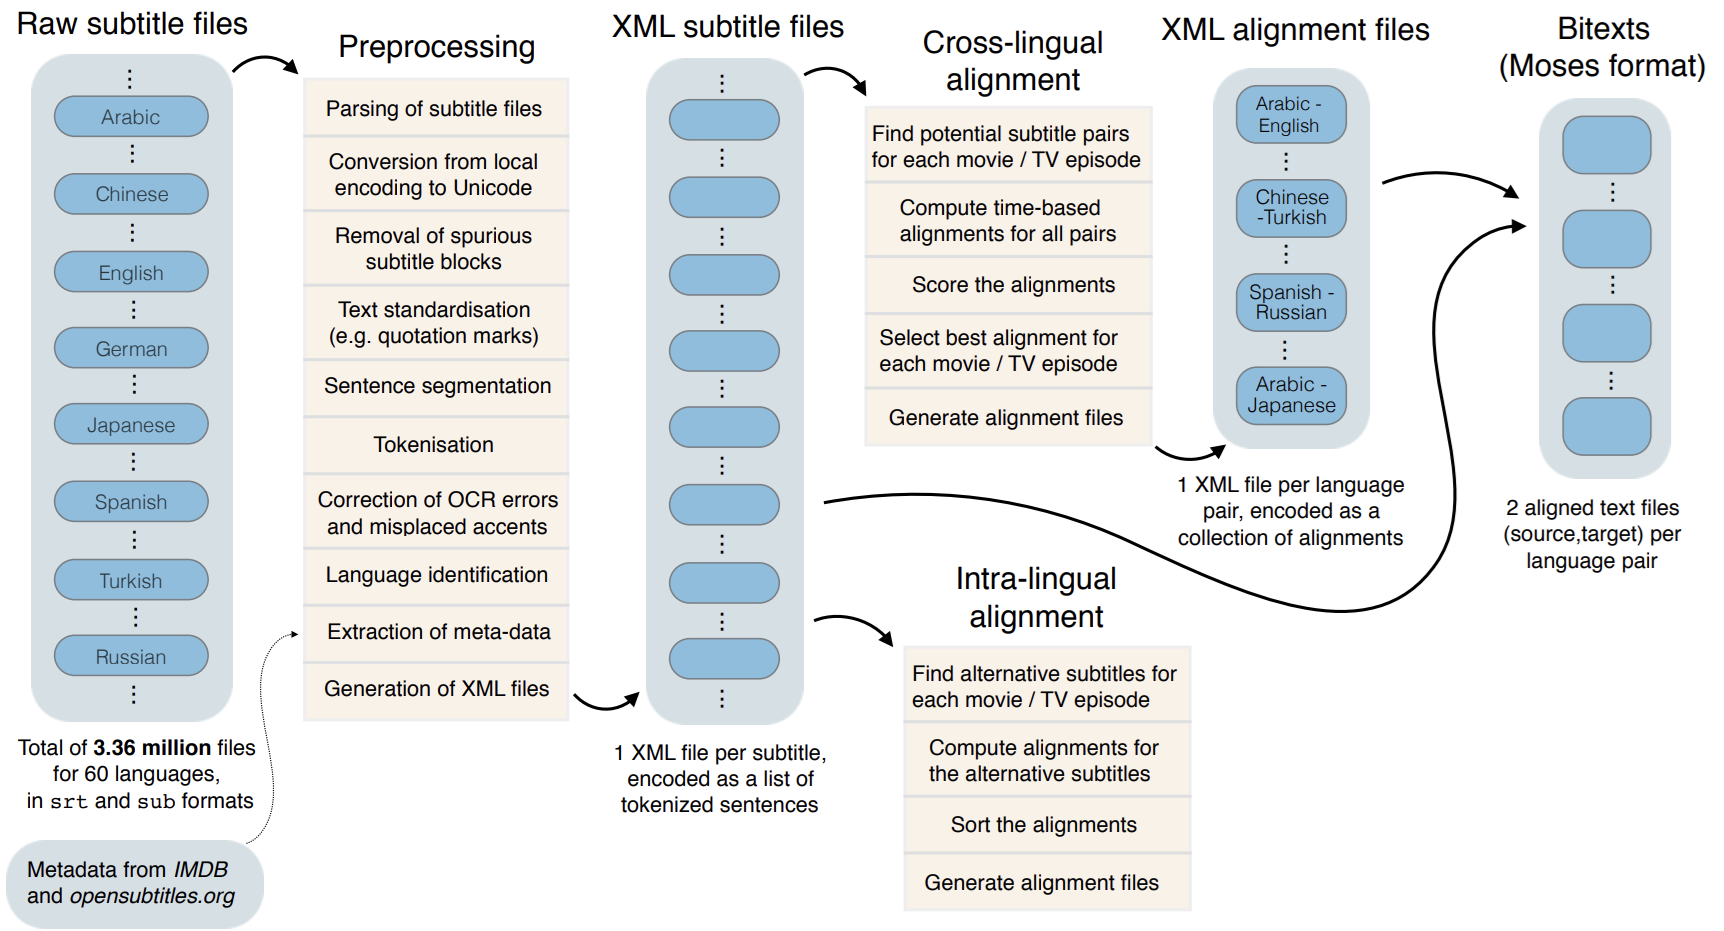
\includegraphics[width=\textwidth]{opensubs_corpus_processing.png}
	\caption{The pipeline producing the OpenSubtitles parallel corpus}
	\label{fig:opensubs pipeline}
\end{figure}

\subsubsection{Wikipedia}
\contentdescription{{
			\begin{itemize}
				\item advantages: diversity of topics, document level corpus which is not copyrighted, regularly updates dumps
				\item disadvantages: language is technical, does not resemble spoken conversation
				\item describe grouping intro multiple scope corpora: describe category structure of Wikipedia
			\end{itemize}
		}}

Wikipedia offers a large amount of data which can be downloaded in the form of dumps at \url{https://dumps.wikimedia.org/}.
In this work, these dumps will be valuable in modeling various linguistic contexts that a language learner might be interested in.

\paragraph{Advantages:}

Wikipedia is a valuable resource for several reasons:
It contains a vast number of articles, from a diverse set of topics.
Wikipedia articles have category assigned to them, which we can use to group articles into linguistic contexts
This means we do not have to assign the articles to topics ourselves, thus enabling the creation of many smaller-scope corpora from Wikipedia with minimal effort.
The characteristics of the article category system on Wikipedia will be discussed in the paragraph below.

Another upshot of Wikipedia is that its articles are licensed under the Creative Commons Attribution-ShareAlike 4.0 International License (\textit{CC BY-SA}).
Because of this, Wikipedia can provide dumps of its entire article database ready for download, with the articles in continuous form and with category metadata attached to them.
This enables us to use the articles as a source for Next Sentence Prediction NSP task.

\paragraph{Disadvantages:}
While Wikipedia offers a large diversity of articles and article topics, the language of the articles follows an academic style of writing.
Thus, the diversity in registers is comparatively low:
Wikipedia is less likely to contain informal language, such as nonstandard language (English: \textit{ain't}, \textit{y'all}) and slang.

Furthermore, it features little language taking conversational form.
% This means that e.g., for English, the second person pronoun "you" occurs very infrequently on Wikipedia. \tocite{Wikipedia rank of you}
This is especially relevant for languages where the certain grammatical forms signify something about the relationship between the speaker and listener:
In Japanese, there exist various linguistic markers of politeness (\textit{Teineigo} and \textit{Keigo}) which play a crucial role in in-person interactions between Japanese speakers, as their presence or absence can signify respect, familiarity or humility with regards to one's interlocutor.
However, such forms are rarely found on Wikipedia, as it does not take the form of a person addressing another person or persons.
Thus, we can see that texts on Wikipedia are of limited use to model linguistic contexts involving in-person conversion.

With these advantages an disadvantages in mind, this work uses Wikipedia articles and their associated metadata to make corpora of various sizes, as will be seen in the next section.

\paragraph{Modeling Linguistic Contexts}

One of the chief advantages of Wikipedia as a corpus its diversity of covered topics.
A language learner who is interested in a particular topic will likely find a matching article category on Wikipedia:
For example, a person with an interest in American cinema who is learning English could likely take vocabulary from the articles of the category "20th-century American actresses" to boost their language learning in that linguistic context.
For this reason, we use a number of manually selected categories as testing grounds for our list generation approach.
For each category, we use a number of articles to make a list, then use different articles from the same category as testing data in the evaluation.
We can thus check if learning vocabulary from a category genuinely prepares a learner in understanding texts from that context.

At the same time, a learner could also wish to make a vocabulary list from concrete Wikipedia articles they would like to read.
For that reason, also use single articles as corpora to be processed by our list generation approach.
In that case, no split of training and test data is necessary, as the aim is not to model general knowledge about a domain, but equip the learner with vocabulary about the \textbf{closed} context of a Wikipedia article.
Therefore in the single-article approach, both the list generation and evaluation use all lines of the article.


% \paragraph{Wikipedia's Category System for Articles}
% There are x categoris on Wikipedia.
% Each article may belong to one or more categories.
% One category can have 0:n parent categories, 0:n child categories.
% Categories therefore not not follow a tree structure, thus most articles belong to more than one top-level category.



\subsubsection{Leipzig Wortschatz Corpora}
Available in x languages

But: data quality issues, methodology might be outdated

\cite{goldhahnBuildingLargeMonolingual2012}

\subsubsection{CCMatrix / NLLB}

% \subsection{Data Augmentation}
% Data Augmentation was not used to gain additional data.
% While in recent years data augmentation methods have become popular for training AI models in NLP, most of these would have either no or a detrimental effect on the methods employed in this paper:
% Some of these methods include \cite{pellicerDataAugmentationTechniques2023}:
% \begin{description}
% 	\item[Character level]
% 	      Introducing character swaps to data is a method used to train the model to noise in the data, but in our case, would only add noise to the results.
% 	\item[Word level]
% 	      There exist techniques to switch words for synonyms or swap words in the sentences to create noise.
% 	      As with noise on the word level, adding words in inappropriate places is undesired for our use case.
% 	      Swapping words for synonyms would also prove detrimental, as this would skew the statistics away from the natural word distribution found in the human-generated source texts.
% \end{description}
% Higher level techniques suffer from the same issues.
% For this reason, the data is left in its "natural state" for our purposes.
%

\section{XAI Methods} \label{sec:xai-methods}
In order to appraise the influence of words in a corpus on the performance of the AI model performing and NLP task, this work employs Explainable AI methods, as explained in chapter \ref{sec:xai-as-tools-of-analysis}.

\subsection{Desiderata}
Chapter \ref{sec:explainable-ai} has explained the use of XAI and stated what kind of XAI methods are especially appropriate for our purpose:
We will employ local, feature attribution XAI methods of both model-specific and model-agnostic type, as these will allow use to gauge the importance of words in the input from multiple points of view.
Model-specific methods have an advantage in that they typically do not require many model calls to attribute importances to features, and take the model structure into account.
On the other hand, model-agnostic methods are useful in that they can be used on any model and gauge the input-output relationship by performing actual experiments on the model, by observing the way changes to input change the output of the model.

In addition to these taxonomical specifications, an ideal XAI method for word extraction should be both accurate in its feature attributions and should not require extensive computation.
Apart from the benefit of attaining faster results, a computationally lightweight approach allows the model to process more data in less time, presumably boosting the accuracy of the resulting utility evaluation.

In the following sections, we will propose several concrete XAI methods for use with the described list generation approach.
The relationship of the XAI methods to the NLP tasks will also be discussed, as not every XAI method is feasible with every tasks, either because of unrealistic amount of computation or because the results of the combination are difficult to evaluate.
The results of the experiments with these methods will be seen in chapter \ref{ch:evaluation}.
\todo{argue against approaches where the input is reduced to BOW, such as SHAP}

\subsection{Model-Agnostic Approaches}
\contentdescription{
	Single Token Ablation, Progressive Summary with
}

\subsubsection{Single Token Ablation}
Our aim in using XAI methods is to find out which words, if known, improve the model's performance the most, when compared to not knowing the word.
Perhaps the simplest way of testing this is by going through every word in the input to the AI model, and checking the model performance when the word is removed from the input.
Within this work, this approach will be known as \textbf{Single Token Ablation}.

\paragraph{Approach:}
Given an input line or pair of lines:
For each word in the input, create a variation of the input where the word is removed.
Run the model on all inputs and measure how much performance is degraded in each case.
Estimated utility is the difference in performance between not removing and removing the word.

\paragraph{Advantages:}
One advantage of Single Token Ablation is its conceptual simplicity, as it is very easy to implement.
Furthermore, its time complexity is fairly minimal for a feature method, as it requires only one model call for each unique token in the sentence ($\mathcal{O}(n)$).

\paragraph{Disadvantages:}
The main downside of this method is that, in long sentences, leaving out a single token will not change the meaning of the sentence to such an extend that the sentence becomes unintelligible.
Assuming the AI model can process sentences with missing words with similar accuracy as humans, the impact on performance may therefore be minimal or not predictive of actual usefulness.
Furthermore, this method does not take into account the utility of a word in the context of word combinations.

\paragraph{Summary:}
Among model-agnostic methods, Single Token Ablation is a computationally inexpensive whose feature perturbation consists of ablating single words.
We may think of this method as simulating a language learner who already knows all words in a sentence except for one, and as such it may not model word utility in such a way that the resulting list is useful for beginners.

\subsubsection{Progressive Summary}
While Single Token Ablation is easy to implement and cheap to execute, its downside is that the performance differences may not be representative of actual utility.
To achieve a more accurate evaluation, we may think of a approach that is in some sense the inverse of removing single words from sentences:
Checking which words are the most essential by reducing the sentence a minimal number of words.

\paragraph{Approach:}
Given an input line, we first let the AI model run on the unaltered input.
We then go through every word in the input line, let the model run with the single word as input, and check which of the words produces an output that is close to the output for the unaltered line.
We can thus see which word summarized the sentence the best.

However, we need not stop here:
After determining the most essential word in the sentence, we can check which words from the remaining pool of words brings the outputs closer still.
By iterating this method, we progressively reconstruct the original sentence, which each step being the best next word to add in order to restore the original output.
For this reason, we will refer to this method as \textbf{Progressive Summary}.
Here, the estimated utility of a word is the boost in performance which is brought to the sentence when the word is added.

\paragraph{Advantages:}
The Progressive Summary approach models the perception of a beginner-level language learner better than Single Token Ablation.
The latter asks which single word, when lacking, degrades performance the most.
Progressive Summary instead asks which words, if known, bring language performance closest to knowing all words in the sentence.

\paragraph{Disadvantages:}
Progressive Summary is much more computationally intensive than Single Token Ablation, which requires only one model call per word in the sentence.
Because of its iterative approach, for a sentence with 10 words, Progressive Summary calls the model $10+9+8+... $ or $\sum_{i=1}^{n}i = \frac{n^2 + n}{2}$ times, which is a time complexity of $\mathcal{O}(n^2)$.


\paragraph{Compatibility with NLP tasks}
As Progressive Summary starts from a set of one words and then progresses to larger sets, it is difficulty to meaningfully employ in combination with an NLP task whose input is not a single line, e.g., Next Sentence Prediction.
One could circumvent the issue by leaving one of the sentences in its original form and only perturbing the other, but this can hardly be seen as a modeling of natural language ability.

\todo{Maybe: Describe issues of using PS with models whose output is single number: Approximating with single words may not be meaningful approximation at all. But should test empirically.}

As such, our implementation Progressive Summary is not used with Next Sentence Prediction.

\paragraph{Summary:}
Progressive Summary attempts to find the most important words in a sentence one by one, by first reducing the sentence to one word, then two etc., and using a distance metric to compare the "summaries" to the original sentence.
The words which bring the model output for the summary closest to that of the original sentence are regarded as the most useful.

\subsection{Model-Specific Methods}
The model-agnostic methods so far are general tools which can be employed on any model.
However, as many of the latest state-of-the-art AI models follow the Neural Network architecture, and more specifically the transformer architecture (see chapter \ref{sec:transformer}), we will also attempt word utility estimation with methods specific to these model.
These model-specific XAI methods have the advantage of being computationally efficient:
Model-agnostic methods extract information about the model by perturbing its inputs and analyzing the resulting changes in the output.
This requires many model calls for one input datum.
In contrast, model-specific methods can analyze the input-output relationship with only one model call, as they look into the model itself for information.
We will therefore try two model-specific methods for analyzing word utility as well, as their more efficient calculations means they can process more input data in a given time, which should increase the accuracy of the resulting word list.

\subsubsection{Attention as Explanation}
One XAI method which has been proposed to explain the decision of transformer models specifically is the transformer's own attention mechanism:
As stated in chapter \ref{sec:transformer}, transformer model use attention to focus on some inputs over others.
This may be used as a kind of explanation, as the inputs which receive more attention presumably contribute more to the model's decision than those with less attention.

\paragraph{Approach:}
Let a transformer model run on an input line.
The transformer will attribution an attention value to each token in the input.
Normalize the attentions such that the attention for all words in the line sums up to one.
The attributed attention to a word is its estimated utility.

\paragraph{Advantages:}
As hinted at before, this method uses one model call for one input line, and thus has a time complexity of $\mathcal{O}(1)$.


\paragraph{Disadvantages:}
One disadvantage of Attention as our attention mechanism is that attentions are attributed to input tokens of the model.
Unlike the black-box methods where word masking is controlled by a tokenizer \textit{independent of the model}, the tokenizer cannot be changed.
AI models are trained with some tokenizer as preprocessing the input, and this tokenizer cannot be changed, lest we change the input format to the AI model itself.
This is an issue because it means that lists generated with the model-specific tokenizer are not necessarily comparable to lists from model-agnostic methods, as the tokenization method may differ.
Additionally, many tokenizer which are used in the preprocessing of models tokenize on a \textit{sub-word} level:

In addition to this technical downside, Attention is controversial as a mechanism to explain model decisions.
\tocite{Attention is not Explanation}

\paragraph{Summary:}


\subsubsection{Layer-wise Relevance Propagation (not yet implemented $\rightarrow$ may be deleted)}
\paragraph{Approach:}
\paragraph{Advantages:}
\paragraph{Disadvantages:}
\paragraph{Summary:}



\chapter{Evaluation} \label{ch:evaluation}
Evaluation of the vocabulary list generation approaches is challenging:
We can measure the quality of each approach by measuring the efficiency of the vocabulary lists it produces.
We have described in detail our method for vocabulary efficiency evaluation in Section \ref{sec:experimental-setup-with-ai}, which involves running an AI model on a context-specific corpus with a given vocabulary, where the vocabulary is given by taking the first $k$ words from the vocabulary list in question.
However, this approach is very similar to our approach for list generation, which involves analyzing AI interaction of AI models with corpora through the use of XAI methods.
Therefore, it is natural to assume that our evaluation approach is biased towards the lists stemming from our list generation approach.
This concern is especially pertinent as it has been shown that AI models do not reliably respond comparably to humans when the inputs to NLP tasks are perturbed \cite{tjuatjaLLMsExhibitHumanlike2024}.
However, to the best of our knowledge, there has not yet been a proposed evaluation metric for vocabulary lists that can be done automatically and which outputs a simple numeric result.

To address this concern, in addition to our own evaluation approach, we also present sample vocabulary lists, use our evaluation approach, and check whether the results align with human intuition.

For this reason, our evaluation is not only concerned with analyzing statistics of measured efficiency, but also with whether the calculated efficiency values are reliable.
The questions examined in this chapter can be summed up as:
\begin{enumerate}
	\item Does our efficiency evaluation of our list correspond with human intuition? (see Section \ref{sec:does-eval-correpond-to-intuition})
	\item According to this efficiency evaluation, do the lists generated by our approach outperform lists from frequency-based approaches? (Sections \ref{sec:results-small-context} and \ref{sec:results-large-context})
	\item Taking all data (list performance, similarity, runtime, etc.) into account, which approach is suited best for which situations? Can we combine the approaches to achieve even better results? (Section \ref{sec:results-discussion})
	      % \item How can the various approaches be combined to supplement each other's weaknesses?
\end{enumerate}

\todo{Add section references when chapter structure is fixed}

The following sections first introduce several baselines against which we compare our list generation approaches.
These baselines include both publicly available vocabulary lists from online language learning tools, and existing list compilation methods introduced in Section \ref{sec:frequency-based-list-generation-methods} in connection with the corpora used for our own lists for a more direct comparison.

We then describe the (numeric) metrics used in the evaluation.
Finally, we present the results of the evaluation, as well as discuss their implications.

\section{Baselines}
It is useful to compare the lists generated by our AI-driven vocabulary list generation approaches with both existing word lists from educational materials, and frequency-based compilation approaches which use the same data as our approaches as input.
They serve as a point of comparison, to see where generated lists agree with existing lists, and to compare the efficiencies of the lists with ours.
For this reason, Section \ref{sec:exising-lists} introduces sources of external lists, and Section \ref{sec:freq-generation-methods-baselines} reviews the frequency-based approaches used as baselines.

\subsection{Existing Vocabulary Lists} \label{sec:exising-lists}
As one point of comparison, we can use existing vocabulary lists that are readily available in digital format, regardless of the method which created them.
For this, a survey was performed on popular language learning tools which make public some of their learning data.
However, as most tools do not publish their vocabulary lists free of cost in text form, we only obtained one list for comparison from the online learning platform \Rosetta\, as the following subsections show.

\subsubsection{Rosetta Stone}
\Rosetta \footnote{\url{https://rosettastone.co.jp/}} is a popular online and mobile language learning platform.
\Rosetta\ publishes some of the course contents on its website \footnote{\url{https://support.rosettastone.com/s/article/Rosetta-Stone-Course-Contents}}.
These lessons take the form of phrases intended to help learners to quickly gain competence in their target language.
To make a list of vocabulary from \Rosetta 's lesson contents, we use the freely available lessons  of the \textit{American English} course (Units 1-20).
We convert the PDF files to text format, filter lines which do not contain lessons contents (e.g., "Lesson 8" and similar ancillary notes).
On the filtered text, we run the \texttt{bert-base-uncased} tokenizer, merge the sub-word tokens to words and let the order of first appearance of a word in the lessons be its rank in the resulting vocabulary list.
Thus, the generated list features the lessons' words in the order in which \Rosetta\ introduces them to its learners, which presumably is close to the word order that \Rosetta\ estimates to be most useful.
One qualification of this statement is that some words may be introduced in order for the learner to have something concrete to talk about, rather than because of their estimated utility.
The final vocabulary list contains 2,545 words in total.

\subsubsection{Unsuitable Sources of Vocabulary Lists}
The following sources of vocabulary lists were considered, but not used for the reasons described below.

\paragraph{Textbooks:}
An obvious source of vocabulary lists to compare our lists against are English textbooks, which often contain vocabulary lists for each lesson.
However, the books we considered as candidates do not publish their course contents free of charge.
This includes:
\begin{itemize}
	\item \textit{Practical English Usage} by Michael Swan \footnote{Available at Oxford University Press at \url{https://elt.oup.com/catalogue/items/global/grammar_vocabulary/practical_english_usage_4th_edition/9780194202510} (last accessed on April 25, 2025)}
\end{itemize}

\paragraph{Cambridge Word Lists:}
Cambridge publishes word lists for certain levels of English \footnote{\url{https://www.cambridgeenglish.org/images/149681-yle-flyers-word-list.pdf}}.
However, these lists are meant for assessing learner's level of vocabulary skills, and the list for each level is ordered by alphabetical order, rather than the perceived level of the word, making them unusable as comparison to our approach.

\paragraph{Duolingo:}
While \textit{Duolingo} \footnote{\url{https://duolingo.com/}} is a popular language platform, it does not publish its course contents in a format that is easily convertible to text and thus be converted to lists of vocabulary.

% This section has introduced some pre-existing lists as points of comparison for our generated vocabulary lists.
% However, one shortcoming of this comparison is that these lists have not been prepared with the same linguistic contexts in mind as those made by this work's approach, and thus their utility is naturally greater in general-context corpora than specialized ones.
% While the context specificity of this work's utility extraction method is a major advance for creating vocabulary lists, it also makes this an unfair comparison.
%
% However, apart from pre-existing lists, there also exist pre-existing \textbf{methods} of finding important words in texts, which we can also use as baselines to compare with our method.
% These also use corpora, but not AI models or XAI methods to find important words.
% The next section introduces some of these methods, which we use to generate comparison lists to our own.


\subsection{Frequency-Based List Generation Methods} \label{sec:freq-generation-methods-baselines}
To gain an impression of how well our XAI-based method for vocabulary list generation performs, we employ the three frequency-based methods for generating lists of vocabulary introduced in Section \ref{sec:frequency-based-list-generation-methods}, namely Raw Frequency, Average Reduced Frequency, and TF-IDF.
We use these three measures as baselines to our methods, again using the tokenizer \texttt{bert-base-uncased} (and merging tokens into words) to divide texts into words that we can count.
To calculate the inverse document frequency in TF-IDF, we use a random sample of 53,178 documents from the Oscar corpus (see Section \ref{sec:oscar}).

One can view these frequency approaches as assigning corpus utility to words in the same way that our AI-driven approaches do, with the corpus utility of a word being given by its frequency/average reduced frequency or TF-IDF.
Therefore, for the large context scenario, their utility aggregation is also performed by summing over the corpus utilities for the single corpora in the large context, as explained in Section \ref{sec:impl-summary-description}.

In this section, we have introduced our baselines, namely the \Rosetta\ vocabulary list, and the three frequency-based list generation methods.
The next section will discuss how we evaluate these baselines, as well as our own various approaches and lists.

% \subsection{LLM Prompt}
% In recent years, Large Language Models have become a popular tools for language learners to find new words to learn about specific areas.
% For this purpose, we run the following prompt to ChatGPT 3 for each context to get a sense of how well our method performs against this easy method.
%
% Prompt:
%
% \begin{lstlisting}[caption={Prompt given to the language model.}, label={lst:blade_runner_prompt}, captionpos=b]
% 	Given a learner of English who knows no English words so far:
% Give me a list of 50 words from the script of the movie "Blade Runner" that they can learn, such that when reading the full script, they have the best understanding of what they are reading.
% Order the list such that the most useful words appear at the top.
% Do not group the words, just generate a raw list.
% Do not number the bullet points. Do not put hyperlinks in the list.
%
% \end{lstlisting}
% \todo{results}


\section{Evaluation Measures}
The various list generation extraction approaches produce ranked lists as outputs.
To compare these, we employ our evaluation approach as described theoretically in Section \ref{sec:experimental-setup-with-ai}.
Section \ref{sec:task-performance-measure} discusses the implementation of this approach.
In addition, we compare the lists by how similar they are to each other in Section \ref{sec:list-similarity-measure}.

\subsection{NLP Task Performance} \label{sec:task-performance-measure}
Our primary metric for evaluating a vocabulary list's efficiency is the approach explained in Section \ref{sec:experimental-setup-with-ai}:
We let an AI model perform an NLP task on a single corpus, using a vocabulary $V_{l, k}$ which consists of the first $k$ elements of the list $l$.
The limited vocabulary is simulated by removing words outside the vocabulary from the inputs to the model.
For illustration, consider again the example sentence:

\begin{quote}
	\textit{Abraham Lincoln faced enmity in 1863.}
\end{quote}

If our vocabulary consists only of the word \textit{enmity}, this sentence becomes:

\begin{quote}
	\textit{Abraham Lincoln enmity 1863.}
\end{quote}

Since \textit{Abraham Lincoln} is recognized as a named entity, we leave it in the input, even though it is not part of the vocabulary.
Non-alphabetic tokens, such as numbers and punctuation, are also left in the input.

Listing \ref{alg:efficiency-evaluation} shows pseudocode for our implementation of the list evaluation approach:

\begin{algorithm}
\caption{Efficient List Generation}
\label{alg:efficiency-evaluation}
\begin{algorithmic}[1]
\Require voc\_list, corpus, model
\State Initialize $vocabulary \gets \emptyset$
\State Initialize $scores \gets []$
\State Set $test\_interval \gets 100$

\For{$i \gets 0$ to $\text{length}(voc\_list)$ step $test\_interval$}
    \State Add $voc\_list[i]$ to $vocabulary$
    \State Initialize $line\_scores \gets []$
    
    \For{each $line$ in $corpus$}
        \State $line\_with\_only\_known\_words \gets$ mask\_words\_not\_in\_vocabulary($line$, $vocabulary$)
        \State $baseline \gets$ model($line$)
        \State $model\_output \gets$ model($line\_with\_only\_known\_words$)
        \State $score \gets$ similarity($baseline$, $model\_output$)
        \State Append $score$ to $line\_scores$
    \EndFor

    \State $avg\_score \gets$ average($line\_scores$)
    \State Append $avg\_score$ to $scores$
\EndFor

\end{algorithmic}
\end{algorithm}


We start the evaluation of every vocabulary list with a vocabulary size of 0, letting the model run on inputs where only named entities and non-alphabetic tokens are left.
The score for the entire corpus is calculated by taking the arithmetic mean of the scores of individual lines.
These runs with a vocabulary size of 0 lets use observe the "utility" of the named entities, putting into context the performance scores when vocabulary is added.
After this, we set the vocabulary size to 10 words, and run the AI models with the resulting vocabulary $V_{l, 10}$.
We then progressively increase the vocabulary by increasing index $k$ by a factor of 4, until we reach the end of the list.
The increase of vocabulary size is exponential, as this ensures a quick evaluation and performance mostly increases at the start of the list, not grow very much towards its end (this is confirmed by the evaluation results shown in Sections \ref{sec:results-small-context} and \ref{sec:results-large-context}).

As stated in Section \ref{sec:sentence-embedding}, we employ the sentence embedding model in the evaluation.
We measure the performance of the model for a sentence variation (with only the words in the vocabulary) by how close the output vector is (in cosine distance) to the output vector of the unaltered sentence.
In order to let the score take on values between 0 and 1, we normalize the line score by also taking the distance between the baseline vector and the model output for an empty string (\texttt{""}).

This approach gives us a direct, quantitative metric for the efficiency of a vocabulary list at each of the test vocabulary sizes.
As an illustration, we present the results of one such efficiency evaluation run for three vocabulary lists on the Wikipedia Article of American actor Marlon Brando \footnote{\url{https://en.wikipedia.org/wiki/Marlon_Brando}} in Figure \ref{fig:marlon-brando-eval}.

\begin{figure}[H]
	\centering
	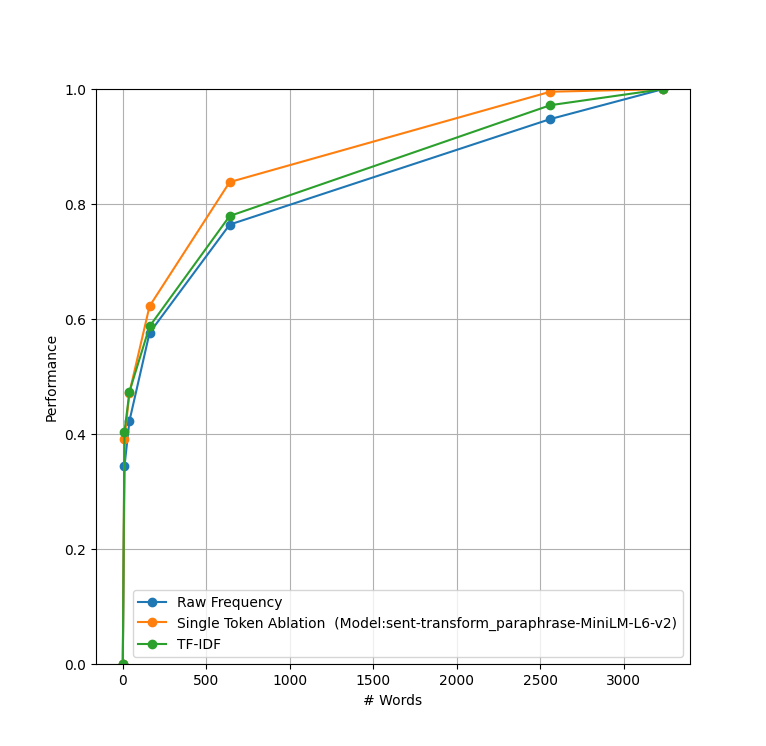
\includegraphics[width=0.5\textwidth]{marlon-brando-eval.png}
	\caption{Efficiency evaluation results on vocabulary lists for the Wikipedia Article of Marlon Brando.}
	\label{fig:marlon-brando-eval}
\end{figure}


To make the figure readable, only three list generation approaches are compared, namely Raw Frequency, TF-IDF, and Single Token Ablation with the sentence embedding model.
We first evaluate the AI model performing the task with a vocabulary size of zero, simulating the state of not knowing any words.
The only tokens in this run are named entities and punctuation, as these are not considered to be potential vocabulary terms.
The vocabularies are then evaluated with an initial size of 10, and increase by a factor of 4 in each step, until a final evaluation is done with the full vocabulary list.
For single corpora, the full list contains all words from the corpus, which is why the performance reaches 1 with all lists.

To compare the results on a broader scale, we aggregate the results of the evaluation runs for each list generation evaluation method as listed in Section \ref{sec:impl-summary-description}.
For both the small context and the large context scenario, we take the average across the lists' scores across the single corpora.
The difference in the scenarios in the evaluation is that for the small context, a list is individually compiled from and evaluated on each single corpus in the large context, whereas for the large scenario, the same vocabulary list is evaluated on all single corpora in the evaluation set of the context (see Section \ref{sec:final-dataset}).

This section has described our approach to evaluating the efficiency of vocabulary lists.
However, as this approach is a novel one, we also compare the \textit{similarity} of the vocabulary lists as a sanity check.
The next section will introduce the metrics we use for this comparison.

\subsection{List Similarity} \label{sec:list-similarity-measure}
Apart from our own vocabulary list evaluation approach that measures the performance of an AI model using the vocabulary list, we also compare how similar the lists are in general.
This allows us to check whether the results of our efficiency evaluation are plausible.
It also serves another purpose, for the case when two approaches for list generation produce vocabulary lists of similar efficiencies, but one takes much less time:
If the lists of both approaches are not only similar in efficiency, but also in content, we can safely say that the approach taking less time is objectively the superior one (for the data observed).

In order to compare the similarity of the resulting vocabulary lists provided by our approaches, metrics are needed that can be consistently calculated across the different approaches.
While a human may be able to qualitatively analyze lists and gain a rough idea of their similarity, computed metrics provide an instantaneous (if simplified) outlook on similarities.
By a metric, we mean a function which takes as parameters two ranked word lists of equal length and outputs a real number giving either a distance or similarity between the lists.

Two considerations influenced our choice of the similarity metrics we employed in our evaluation:
Firstly, the metrics must be \textbf{able to handle elements which occur in only one of the two lists}.
Secondly, differences between elements at \textbf{the tops of the lists must impact the metric more} than differences between elements at the ends.
This is because the top of each vocabulary list contains the words which are ranked as most important.

While Kendall rank correlation \cite{kendallNewMeasureRank1938c} and Spearman's footrule  \cite{spearmanCorrelationCalculatedFaulty1910} are simple metrics to compare ranked lists, they make no distinction between differences at the tops of lists and differences at their ends, in addition to being difficult to adapt to handle for missing elements.
Instead, we use two metrics called Average Overlap and Normalized Discounted Cumulative Gain, which we introduce in the following subsections.
%
% \subsubsection{Sequential rank agreement (modified)}
% Sequential rank agreement \cite{ekstromSequentialRankAgreement2015} is based on the deviations of some subset of the lists in the upper ranks.
% 	      It is important to note that this metric has an additional parameter "depth" which determines how many elements (from the top of the list) are considered.
% 	      It is therefore more helpful to view its results at various depths.
% 	      The original formula for this metric in the case of two lists is:
% 	      \[
% 		      a_{d} := a \text{ from start to rank } d
% 	      \]
%
% 	      \[
% 		      S_{d} := a_{d} \cup b_{d}
% 	      \]
%
% 	      \[
% 		      SRA_{d}(a, b) := \lambda \cdot \frac{\sum_{x \in S_{d}} \sigma ^2 \left( \left( r_{b}(x) \right) - \left( r_{a}(x) \right) \right)}{|S_{d}|}
% 	      \]
%
% 	      where \(\lambda\) is a normalization factor ensuring that \(\max(SRA) = 1\).
% 	      In its proposed form, this metric can only compare lists which contain the same set of unique elements, just in different orders.
% 	      In order to make it work on lists where this is not the case, one can set the "rank" of nonexisting elements to a value greater than the length of the lists, such as \(2 |a|\).
% 	      Another drawback of the metric is that the standard deviation of two numbers does not depend on their absolute value, only their difference.
% 	      However, to satisfy number 3 of the stated requirements, we can take the deviation of the logarithm of the ranks instead of the deviation of the ranks themselves, resulting in the formula
%
% 	      \[
% 		      r^{\prime}(x) :=
% 		      \begin{cases}
% 			      \mathrm{rank}_{b}(x) & \text{if } x \in b, \\
% 			      2 \cdot |a|          & \text{otherwise.}
% 		      \end{cases}
% 	      \]
%
% 	      \[
% 		      SRA^{mod}_{d}(a, b) := \lambda \cdot \frac{\sum_{x \in S_{d}} \sigma ^2 \left( \log (r^{\prime}_{b}(x))-\log(r^{\prime}_{a}(x))\right)}{|S_{d}|}
% 	      \]
%
% 	      For this modified version, \(\lambda\) can be calculated with:
%
% 	      \[
% 		      \lambda = \frac{1}{SRA_{d}(a, a^{*})},
% 	      \]
%
% 	      where \(a^{*}\) is a list such that \(a \cap a^{*} = \emptyset\).

\subsubsection{Average Overlap}
The Average Overlap \cite{webberSimilarityMeasureIndefinite2010} of two lists is given by the average cardinality of the intersection (overlap) of the sets given by taking the two lists up until every possible index.
Because the first element contributes to every iteration, it causes the tops of the lists to impact the metrics more than their ends.
There is also no issue with partial overlaps between the lists.
Using the notation of a vocabulary $V_{l, k}$ as a set of words given by vocabulary list $l$ until an index $k$ (see Section \ref{sec:voc-list-efficiency}), the average overlap between two vocabulary lists like is given by:

\begin{equation}
	\text{AverageOverlap}(A, B) = \frac{1}{n} \sum_{k=1}^{n} \frac{|V_{A, k}  \cap V_{B,k}|}{k}
\end{equation}

% \item \textbf{11-point interpolated average precision} \cite{manningIntroductionInformationRetrieval2008}: Uses set metric precision (though may also use recall or F1 score on various subsets of the list (first 10\%, first 20\% etc.) and takes their geometric mean to arrive at a single number.
%       As each of the elevent numbers is calculated on the partial subset of the list's elements starting at the first element, this means that changes in the top of the list affect more of these numbers and thus have a larger impact on the final calculated mean.
%       One drawback of this method is that precision measurement within the 10\% interval only takes into account set membership, not the order of words:
%       For a list containing 10,000 words, the evaluated intervals are words in the index intervals $\left[ 0, 1000 \right), \left[ 0, 2000 \right), ... ,\left[ 0, 10000 \right)$.  Differences of order within the first 1000 words are thus ignored.

\subsubsection{Normalized Discounted Cumulative Gain (NCDG)}
(Normalized) Discounted Cumulative Gain \cite{jurafskySpeechLanguageProcessing2025} is a metric used in information retrieval to compare relevance scoring of two sets of elements.
By making the relevance score $R$ of a set element determined by its rank in our ranked lists, we adapt this metric to compare the similarity of two lists:

% This formula outputs a value between 0 and 1, with 1 being given if both lists are identical, 0 when they have no elements in common, and values in between when there is partial overlap between elements and/or their order is different.

% ${DCG_{p}} =\sum _{i=1}^{p}{\frac {rel_{i}}{\log _{2}(i+1)}}=rel_{1}+\sum _{i=2}^{p}{\frac {rel_{i}}{\log _{2}(i+1)}}$



\[
	\text{DCG}(A, B) = \sum_{k=1}^{n} \frac{2^{R(A_k)} - 1}{\log_2(1 + k)}
\]

The relevance $R_B$ is a function taking as input an element (not an index) of list A.
We define it as follows:

\[
	R_B(m) :=
	\begin{cases}
		\frac{1}{rank_{B}(m) + 1} & \text{if } B \text{ contains } m \\
		0                         & \text{otherwise}
	\end{cases}
\]
With relevance defined in this way, we ensure both that differences between the tops of the lists impact the measurement more than differences at the end, and the handling of elements which only appear in one of the two lists.
To normalize this metric to output values between 0 and 1, we divide by the maximum value for the list length, which is given by the DCG of one of the lists with itself:

\[
	\text{NDCG}(A,B) = \frac{1}{\text{DCG}(A, A)} \text{DCG}(A, B)
\]

Having established our metrics to evaluate both the performance of and similarity between vocabulary lists, we present the results of the evaluation in the following section.

\section{Results} \label{sec:results}
This section presents the results both for the small context and large context scenarios.
The list generation approaches are evaluated by the performance of their lists on NLP tasks, by the similarity between the lists, and by the time required to generate them.

We first establish that our approach to evaluating list efficiency does roughly align with human intuition in Section \ref{sec:does-eval-correpond-to-intuition}.
After this, we show the results for approaches in the small context scenario where lists are compiled and tested on single Wikipedia articles and subtitles in Section \ref{sec:results-small-context}, where we find that our AI-driven approaches generally outperform the baselines.
Finally, the results for the large contexts (using separate single corpora for generation and evaluation) are presented in Section \ref{sec:results-large-context}.
For the large contexts, we find that most list generation approaches produce lists of similar efficiencies, which seems to imply that frequency is a valid proxy metric for large vocabulary sizes, as it requires less time for vocabulary list generation. 

\subsection{Correspondence of Efficiency Evaluation with Human Intuition} \label{sec:does-eval-correpond-to-intuition}
As mentioned in the introduction to this chapter, we use the performance of AI models on corpora where we simulate a limited vocabulary in order to measure the efficiency of a vocabulary list.
Before we present the results of these tests, however, we examine whether the performance of AI models is a reliable indicator that the list is useful to humans as well.
This section therefore examines several vocabulary lists tested on a short sample text containing ten lines of dialog from the subtitles of the 1972 movie \textit{The Godfather}, seen here:

\begin{lstlisting}[caption={
Sample text.
}, label={lst:sample-text-original}
, captionpos=b]
Moe loves the business.
He never said nothing about selling.
I'll make him an offer he can't refuse.
See, Johnny...
We figure that entertainment would draw gamblers to the casino.
We hope you'll sign a contract to appear five times a year.
Perhaps convince some of your friends in the movies to do the same.
We're counting on you.
Sure, Mike.
I'll do anything for my godfather.
\end{lstlisting}




The following shows the text leaving only the named entities and punctuation tokens, which constitutes our starting point for the evaluation.
An evaluation score for each line is displayed on the left:


\begin{lstlisting}[caption={
Sample text with no vocabulary. Total score: 0.17.
}, label={lst:sample-text-empty}
, captionpos=b]
0.0	                      .
0.0	                                   .
0.0	 '                            '         .
0.9	   ,johnny...
0.0	                                                              .
0.0	           '                                               .
0.0	                                                                  .
0.0	  '                   .
0.8	    ,mike.
0.0	 '                                .
\end{lstlisting}




Due to the uncased tokenizer used, all words in the reconstructed text are lowercase.
We can see that the lines containing named entities (Line 4 and 9) already have a rather high score in the evaluation, reflecting the importance of the names to the meaning of the sentences.
The other lines receive a score of 0.0, resulting in an overall score of 0.17.
We also observe that the name \textit{Moe} in line 1 is not recognized by the Named Entity Recognition model, (falsely) making it a possible vocabulary word.

To compare their intuitive utilities, we use four vocabulary lists on the corpus and see how well their first words perform when evaluated on the sample text:
\begin{enumerate}
	\item A randomly ordered list from words in the sample text.
	\item A list compiled with raw frequency.
	\item A list compiled with TF-IDF (with the Oscar corpus as normalization).
	\item A list compiled by Single Token Summary with sentence embedding.
\end{enumerate}

The tops of the lists can be seen in Table \ref{tbl:first-k-words-sample}.

\begin{table}[H]
	\centering
	\begin{tabular}{lllll}
\toprule
 & \rotatebox{90}{Random} & \rotatebox{90}{Raw Frequency} & \rotatebox{90}{TF-IDF} & \rotatebox{90}{Single Token Summary - Sent. Emb.} \\
\midrule
0 & i & the & moe & moe \\
1 & a & ll & godfather & casino \\
2 & selling & we & gamblers & godfather \\
3 & same & to & ll & gamblers \\
4 & contract & he & convince & counting \\
5 & make & i & counting & offer \\
6 & draw & you & casino & refuse \\
7 & of & a & refuse & ll \\
8 & appear & do & loves & contract \\
9 & casino & moe & draw & movies \\
\bottomrule
\end{tabular}
	\caption{Top 10 words of each compared list on the sample text.}
	\label{tbl:first-k-words-sample}
\end{table}

It can be seen that the ten top words of the lists collected with TF-IDF and the Single Token Summary approach give a better idea of the meaning of the text than the words from the random and raw frequency lists.
Next, we examine the words in the context of the sample text.
In the following listings, we see the sample text with the 10 top words filled in from each vocabulary list, in addition to the recognized named entities.
Each line displays the evaluation score for it, and the total score (calculated by taking the average across the lines) is seen in the caption of each listing:


\begin{lstlisting}[caption={
Sample text with 10 words from the Random list. Total score: 0.3.
}, label={lst:sample-text-random}
, captionpos=b]
0.0	                      .
0.2	                            selling.
0.0	i'    make                    '         .
0.9	   ,johnny...
0.7	                                   draw                 casino.
0.3	           '         a contract    appear            a     .
0.1	                      of                                      same.
0.0	  '                   .
0.8	    ,mike.
0.1	i'                                .
\end{lstlisting}




\begin{lstlisting}[caption={
Sample text with 10 words from the Raw Frequency list. Total score: 0.33.
}, label={lst:sample-text-frequency}
, captionpos=b]
0.6	moe       the         .
0.1	he                                 .
0.3	i' ll                   he    '         .
0.9	   ,johnny...
0.1	we                                               to the       .
0.1	we      you' ll      a          to                   a     .
0.1	                                         the        to do the     .
0.3	we'                you.
0.8	    ,mike.
0.2	i' ll do                          .
\end{lstlisting}




\begin{lstlisting}[caption={
Sample text with 10 words from the TF-IDF list. Total score: 0.52.
}, label={lst:sample-text-tf-idf}
, captionpos=b]
0.8	moe loves             .
0.0	                                   .
0.5	 ' ll                         '   refuse.
0.9	   ,johnny...
0.7	                                   draw gamblers        casino.
0.1	           ' ll                                            .
0.3	        convince                                                  .
0.5	  '    counting       .
0.8	    ,mike.
0.6	 ' ll                    godfather.
\end{lstlisting}




\begin{lstlisting}[caption={
Sample text with 10 words from the Single Token Summary list. Total score: 0.56.
}, label={lst:sample-text-single-token-summary}
, captionpos=b]
0.7	moe                   .
0.0	                                   .
0.7	 ' ll             offer       '   refuse.
0.9	   ,johnny...
0.7	                                        gamblers        casino.
0.4	           ' ll        contract                            .
0.4	                                             movies               .
0.5	  '    counting       .
0.8	    ,mike.
0.6	 ' ll                    godfather.
\end{lstlisting}




The main observation is that the texts with the TF-IDF and Single Token Summary, whose top words make the meaning of the text much closer to the meaning of the original text than those of the other two approaches, are indeed evaluated significantly higher (0.52 and 0.56 vs. 0.33 and 0.30).
In our opinion, this is evidence that our evaluation scores roughly coincide with how much the words let a reader understand the text, aligning with utility as defined in Section \ref{sec:utility}.
Both of these lists feature the essential words \textit{casino}, \textit{godfather} and \textit{gamblers}, as well as other words which let a reader guess at the situation.

We can, however, also notice some peculiarities in the evaluation scores:
The text with words from the randomly assembled list (Listing \ref{lst:sample-text-random}) seems more understandable to us than when words from the  frequency list are filled in (Listing \ref{lst:sample-text-frequency}), since the randomly compiled list contains useful words such as \textit{selling}, \textit{casino} and \textit{contract}.
However, the text with the frequency words receives a higher evaluation score than the one with the random words (0.33 vs. 0.3).
This is due partially to the unrecognized entity \textit{moe}, which is contained in the frequency list but not the random one, "artificially" boosting the score of the frequency list.
But even disregarding that name, the scores are not as disparate as we expected them to be:
For example, line 3 in the random words text \texttt{"i' make       ."} receives a (rounded) score of 0.0, while the same line in the frequency text \texttt{"i' ll      he      ."} is assigned a score of 0.3.
Since both versions of the line seem to contain very little information, this difference in the evaluation score suggests that the cosine distances between the sentence embeddings do not completely correlate with differences in meaning of the sentences, and thus the evaluation scores may not reflect the true utility of words in all circumstances.
With these observations in mind, we present the evaluation results in the next sections.

\subsection{Small Context} \label{sec:results-small-context}
This section shows the evaluation results of the vocabulary lists for the small context scenario, where each list is generated from a single corpus (single article or subtitles) and then evaluated on that same corpus.
We evaluate the efficiencies of the lists, their similarities, and the time needed to compile them.
Each of the approaches from \ref{sec:impl-summary-description} is evaluated, as well as the three frequency-based approaches.
We do not include the \Rosetta\ list in the comparison, as it is too generic to be compared against lists specifically compiled for a short context.
Instead, the \Rosetta\ list is used in the next section, showing the results for the large context scenario.

% Table \ref{tbl:performance-results-single-opensubs} and \ref{tbl:performance-results-single-wikipedia} show the aggregated results of single corpora, separated by corpus type.

\subsubsection{List Efficiency}
This section shows and discusses the efficiencies of the lists generated by each generation approach , as evaluated with the sentence embedding model (see Section \ref{sec:task-performance-measure}).
The following tables show the results , at the test vocabulary sizes, with warm colors indicating higher efficiency.
The highest score at each vocabulary size is highlighted in \textbf{bold} font.
Performance scores were rounded to two decimals to improve readability.

\begin{table}[H]
        \centering
        \resizebox{\textwidth}{!}{%
    \begin{tabular}{lrrrrr}
\toprule
 & Size=0 & Size=10 & Size=40 & Size=160 & Size=640 \\
\midrule
Raw Frequency & \cellcolor[RGB]{58,76,192}\textbf{0.17} & \cellcolor[RGB]{82,110,220}0.23 & \cellcolor[RGB]{142,177,253}0.37 & \cellcolor[RGB]{241,202,182}0.64 & \cellcolor[RGB]{202,61,56}0.90 \\
Average Reduced Frequency & \cellcolor[RGB]{58,76,192}\textbf{0.17} & \cellcolor[RGB]{82,110,220}0.23 & \cellcolor[RGB]{141,175,253}0.36 & \cellcolor[RGB]{239,206,188}0.62 & \cellcolor[RGB]{202,61,56}0.90 \\
TF-IDF & \cellcolor[RGB]{58,76,192}\textbf{0.17} & \cellcolor[RGB]{91,121,228}0.25 & \cellcolor[RGB]{151,184,254}0.38 & \cellcolor[RGB]{241,202,182}0.64 & \cellcolor[RGB]{198,53,52}0.91 \\
Attention - Sent. Emb. & \cellcolor[RGB]{58,76,192}\textbf{0.17} & \cellcolor[RGB]{91,121,228}0.25 & \cellcolor[RGB]{153,186,254}0.39 & \cellcolor[RGB]{244,194,170}0.66 & \cellcolor[RGB]{188,31,44}0.93 \\
Single Token Ablation - Sent. Emb. & \cellcolor[RGB]{58,76,192}\textbf{0.17} & \cellcolor[RGB]{96,128,232}0.26 & \cellcolor[RGB]{163,193,254}0.41 & \cellcolor[RGB]{246,186,159}\textbf{0.68} & \cellcolor[RGB]{179,3,38}\textbf{0.95} \\
Single Token Summary - Sent. Emb. & \cellcolor[RGB]{58,76,192}\textbf{0.17} & \cellcolor[RGB]{97,130,234}\textbf{0.27} & \cellcolor[RGB]{163,193,254}\textbf{0.41} & \cellcolor[RGB]{246,189,164}0.67 & \cellcolor[RGB]{185,22,42}0.94 \\
Progressive Summary - Sent. Emb. & \cellcolor[RGB]{58,76,192}\textbf{0.17} & \cellcolor[RGB]{95,126,231}0.26 & \cellcolor[RGB]{159,190,254}0.40 & \cellcolor[RGB]{245,192,167}0.67 & \cellcolor[RGB]{184,17,41}0.94 \\
\midrule 
\textbf{[Mean]} & \textbf{0.17} & \textbf{0.25} & \textbf{0.39} & \textbf{0.65} & \textbf{0.92} \\
\bottomrule
\end{tabular}
    }
        \caption{Efficiencies of vocabulary lists on single OPUS subtitles.}\end{table}
\begin{table}[H]
        \centering
        \resizebox{\textwidth}{!}{%
    \begin{tabular}{lrrrrr}
\toprule
 & Size=0 & Size=10 & Size=40 & Size=160 & Size=640 \\
\midrule
Raw Frequency & \cellcolor[RGB]{58,76,192}\textbf{0.46} & \cellcolor[RGB]{90,120,227}0.52 & \cellcolor[RGB]{153,186,254}0.61 & \cellcolor[RGB]{239,205,187}0.76 & \cellcolor[RGB]{215,84,68}0.92 \\
Average Reduced Frequency & \cellcolor[RGB]{58,76,192}\textbf{0.46} & \cellcolor[RGB]{86,115,224}0.51 & \cellcolor[RGB]{145,179,254}0.60 & \cellcolor[RGB]{236,210,196}0.75 & \cellcolor[RGB]{215,84,68}0.92 \\
TF-IDF & \cellcolor[RGB]{58,76,192}\textbf{0.46} & \cellcolor[RGB]{130,165,251}0.58 & \cellcolor[RGB]{188,209,246}0.66 & \cellcolor[RGB]{244,196,173}0.78 & \cellcolor[RGB]{205,66,58}0.94 \\
Attention - Sent. Emb. & \cellcolor[RGB]{58,76,192}\textbf{0.46} & \cellcolor[RGB]{97,130,234}0.53 & \cellcolor[RGB]{164,194,254}0.63 & \cellcolor[RGB]{245,192,167}0.79 & \cellcolor[RGB]{197,50,51}0.95 \\
Single Token Ablation - NSP & \cellcolor[RGB]{58,76,192}\textbf{0.46} & \cellcolor[RGB]{88,118,226}0.51 & \cellcolor[RGB]{127,162,250}0.57 & \cellcolor[RGB]{220,220,221}0.72 & \cellcolor[RGB]{210,75,63}0.93 \\
Single Token Ablation - Sent. Emb. & \cellcolor[RGB]{58,76,192}\textbf{0.46} & \cellcolor[RGB]{134,169,252}0.58 & \cellcolor[RGB]{197,213,242}0.68 & \cellcolor[RGB]{246,164,134}\textbf{0.83} & \cellcolor[RGB]{179,3,38}\textbf{0.97} \\
Single Token Summary - NSP & \cellcolor[RGB]{58,76,192}\textbf{0.46} & \cellcolor[RGB]{107,141,240}0.54 & \cellcolor[RGB]{157,189,254}0.61 & \cellcolor[RGB]{225,218,214}0.73 & \cellcolor[RGB]{229,112,87}0.89 \\
Single Token Summary - Sent. Emb. & \cellcolor[RGB]{58,76,192}\textbf{0.46} & \cellcolor[RGB]{139,174,253}\textbf{0.59} & \cellcolor[RGB]{201,215,238}\textbf{0.68} & \cellcolor[RGB]{247,174,145}0.82 & \cellcolor[RGB]{194,45,49}0.95 \\
Progressive Summary - Sent. Emb. & \cellcolor[RGB]{58,76,192}\textbf{0.46} & \cellcolor[RGB]{124,160,249}0.57 & \cellcolor[RGB]{190,211,245}0.67 & \cellcolor[RGB]{247,176,146}0.82 & \cellcolor[RGB]{187,26,43}0.96 \\
\midrule 
\textbf{[Mean]} & \textbf{0.46} & \textbf{0.55} & \textbf{0.63} & \textbf{0.78} & \textbf{0.94} \\
\bottomrule
\end{tabular}
    }
        \caption{Efficiencies of vocabulary lists on single articles in Wikipedia category \textit{1980s English-language films}.}\end{table}
\begin{table}[H]
        \centering
        \resizebox{\textwidth}{!}{%
    \begin{tabular}{lrrrrr}
\toprule
 & Size=0 & Size=10 & Size=40 & Size=160 & Size=640 \\
\midrule
Raw Frequency & \cellcolor[RGB]{58,76,192}\textbf{0.54} & \cellcolor[RGB]{117,152,246}0.61 & \cellcolor[RGB]{189,210,246}0.70 & \cellcolor[RGB]{245,192,167}0.81 & \cellcolor[RGB]{219,92,74}0.92 \\
Average Reduced Frequency & \cellcolor[RGB]{58,76,192}\textbf{0.54} & \cellcolor[RGB]{116,151,245}0.61 & \cellcolor[RGB]{185,208,248}0.70 & \cellcolor[RGB]{244,195,171}0.81 & \cellcolor[RGB]{220,94,75}0.91 \\
TF-IDF & \cellcolor[RGB]{58,76,192}\textbf{0.54} & \cellcolor[RGB]{148,181,254}0.65 & \cellcolor[RGB]{208,218,233}0.73 & \cellcolor[RGB]{247,181,152}0.83 & \cellcolor[RGB]{211,77,64}0.93 \\
Attention - Sent. Emb. & \cellcolor[RGB]{58,76,192}\textbf{0.54} & \cellcolor[RGB]{126,161,249}0.62 & \cellcolor[RGB]{201,215,238}0.72 & \cellcolor[RGB]{247,173,143}0.84 & \cellcolor[RGB]{201,59,55}0.94 \\
Single Token Ablation - NSP & \cellcolor[RGB]{58,76,192}\textbf{0.54} & \cellcolor[RGB]{111,145,242}0.61 & \cellcolor[RGB]{164,194,254}0.67 & \cellcolor[RGB]{240,204,185}0.79 & \cellcolor[RGB]{216,86,70}0.92 \\
Single Token Ablation - Sent. Emb. & \cellcolor[RGB]{58,76,192}\textbf{0.54} & \cellcolor[RGB]{155,187,254}0.66 & \cellcolor[RGB]{222,219,218}0.75 & \cellcolor[RGB]{240,139,109}\textbf{0.87} & \cellcolor[RGB]{179,3,38}\textbf{0.97} \\
Single Token Summary - NSP & \cellcolor[RGB]{58,76,192}\textbf{0.54} & \cellcolor[RGB]{138,173,253}0.64 & \cellcolor[RGB]{193,212,244}0.71 & \cellcolor[RGB]{241,202,182}0.79 & \cellcolor[RGB]{235,127,99}0.89 \\
Single Token Summary - Sent. Emb. & \cellcolor[RGB]{58,76,192}\textbf{0.54} & \cellcolor[RGB]{164,194,254}\textbf{0.67} & \cellcolor[RGB]{225,218,214}\textbf{0.76} & \cellcolor[RGB]{243,150,120}0.86 & \cellcolor[RGB]{196,48,50}0.95 \\
Progressive Summary - Sent. Emb. & \cellcolor[RGB]{58,76,192}\textbf{0.54} & \cellcolor[RGB]{148,181,254}0.65 & \cellcolor[RGB]{215,219,226}0.74 & \cellcolor[RGB]{243,152,121}0.86 & \cellcolor[RGB]{190,35,45}0.95 \\
\midrule 
\textbf{[Mean]} & \textbf{0.54} & \textbf{0.64} & \textbf{0.72} & \textbf{0.83} & \textbf{0.93} \\
\bottomrule
\end{tabular}
    }
        \caption{Efficiencies of vocabulary lists on single articles in Wikipedia category \textit{20th-century American actresses}.}\end{table}
\begin{table}[H]
        \centering
        \resizebox{\textwidth}{!}{%
    \begin{tabular}{lrrrrr}
\toprule
 & Size=0 & Size=10 & Size=40 & Size=160 & Size=640 \\
\midrule
Raw Frequency & \cellcolor[RGB]{58,76,192}\textbf{0.53} & \cellcolor[RGB]{99,131,234}0.59 & \cellcolor[RGB]{168,197,253}0.68 & \cellcolor[RGB]{242,199,178}0.80 & \cellcolor[RGB]{218,90,72}0.91 \\
Average Reduced Frequency & \cellcolor[RGB]{58,76,192}\textbf{0.53} & \cellcolor[RGB]{97,130,234}0.59 & \cellcolor[RGB]{164,194,254}0.67 & \cellcolor[RGB]{240,204,185}0.79 & \cellcolor[RGB]{220,94,75}0.91 \\
TF-IDF & \cellcolor[RGB]{58,76,192}\textbf{0.53} & \cellcolor[RGB]{133,168,251}0.63 & \cellcolor[RGB]{190,211,245}0.70 & \cellcolor[RGB]{246,188,162}0.81 & \cellcolor[RGB]{210,75,63}0.92 \\
Attention - Sent. Emb. & \cellcolor[RGB]{58,76,192}\textbf{0.53} & \cellcolor[RGB]{108,142,241}0.60 & \cellcolor[RGB]{180,205,250}0.69 & \cellcolor[RGB]{246,183,156}0.82 & \cellcolor[RGB]{200,56,53}0.94 \\
Single Token Ablation - NSP & \cellcolor[RGB]{58,76,192}\textbf{0.53} & \cellcolor[RGB]{97,130,234}0.59 & \cellcolor[RGB]{142,177,253}0.64 & \cellcolor[RGB]{233,212,201}0.77 & \cellcolor[RGB]{218,90,72}0.91 \\
Single Token Ablation - Sent. Emb. & \cellcolor[RGB]{58,76,192}\textbf{0.53} & \cellcolor[RGB]{137,172,252}0.64 & \cellcolor[RGB]{206,217,235}0.72 & \cellcolor[RGB]{243,152,121}\textbf{0.85} & \cellcolor[RGB]{179,3,38}\textbf{0.96} \\
Single Token Summary - NSP & \cellcolor[RGB]{58,76,192}\textbf{0.53} & \cellcolor[RGB]{117,152,246}0.61 & \cellcolor[RGB]{168,197,253}0.68 & \cellcolor[RGB]{231,214,204}0.77 & \cellcolor[RGB]{237,132,103}0.88 \\
Single Token Summary - Sent. Emb. & \cellcolor[RGB]{58,76,192}\textbf{0.53} & \cellcolor[RGB]{144,178,254}\textbf{0.65} & \cellcolor[RGB]{210,218,231}\textbf{0.73} & \cellcolor[RGB]{245,161,130}0.84 & \cellcolor[RGB]{196,48,50}0.94 \\
Progressive Summary - Sent. Emb. & \cellcolor[RGB]{58,76,192}\textbf{0.53} & \cellcolor[RGB]{133,168,251}0.63 & \cellcolor[RGB]{199,214,240}0.71 & \cellcolor[RGB]{246,167,137}0.84 & \cellcolor[RGB]{190,35,45}0.95 \\
\midrule 
\textbf{[Mean]} & \textbf{0.53} & \textbf{0.61} & \textbf{0.69} & \textbf{0.81} & \textbf{0.92} \\
\bottomrule
\end{tabular}
    }
        \caption{Efficiencies of vocabulary lists on single articles in Wikipedia category \textit{20th-century American male actors}.}\end{table}
\begin{table}[H]
        \centering
        \resizebox{\textwidth}{!}{%
    \begin{tabular}{lrrrrr}
\toprule
 & Size=0 & Size=10 & Size=40 & Size=160 & Size=640 \\
\midrule
Raw Frequency & \cellcolor[RGB]{58,76,192}\textbf{0.53} & \cellcolor[RGB]{93,125,230}0.58 & \cellcolor[RGB]{157,189,254}0.65 & \cellcolor[RGB]{235,211,198}0.75 & \cellcolor[RGB]{216,86,70}0.88 \\
Average Reduced Frequency & \cellcolor[RGB]{58,76,192}\textbf{0.53} & \cellcolor[RGB]{93,125,230}0.58 & \cellcolor[RGB]{153,186,254}0.64 & \cellcolor[RGB]{230,215,207}0.74 & \cellcolor[RGB]{222,98,78}0.87 \\
TF-IDF & \cellcolor[RGB]{58,76,192}\textbf{0.53} & \cellcolor[RGB]{130,165,251}0.62 & \cellcolor[RGB]{182,206,249}0.68 & \cellcolor[RGB]{242,200,179}0.77 & \cellcolor[RGB]{210,75,63}0.89 \\
Attention - Sent. Emb. & \cellcolor[RGB]{58,76,192}\textbf{0.53} & \cellcolor[RGB]{104,137,238}0.59 & \cellcolor[RGB]{164,194,254}0.66 & \cellcolor[RGB]{239,205,187}0.76 & \cellcolor[RGB]{204,63,57}0.90 \\
Single Token Ablation - NSP & \cellcolor[RGB]{58,76,192}\textbf{0.53} & \cellcolor[RGB]{99,131,234}0.58 & \cellcolor[RGB]{133,168,251}0.62 & \cellcolor[RGB]{205,217,236}0.70 & \cellcolor[RGB]{226,106,83}0.86 \\
Single Token Ablation - Sent. Emb. & \cellcolor[RGB]{58,76,192}\textbf{0.53} & \cellcolor[RGB]{126,161,249}0.61 & \cellcolor[RGB]{188,209,246}0.68 & \cellcolor[RGB]{246,182,154}\textbf{0.79} & \cellcolor[RGB]{179,3,38}\textbf{0.92} \\
Single Token Summary - NSP & \cellcolor[RGB]{58,76,192}\textbf{0.53} & \cellcolor[RGB]{115,149,244}0.60 & \cellcolor[RGB]{159,190,254}0.65 & \cellcolor[RGB]{216,219,225}0.72 & \cellcolor[RGB]{242,147,117}0.83 \\
Single Token Summary - Sent. Emb. & \cellcolor[RGB]{58,76,192}\textbf{0.53} & \cellcolor[RGB]{137,172,252}\textbf{0.62} & \cellcolor[RGB]{195,213,242}\textbf{0.69} & \cellcolor[RGB]{246,183,156}0.79 & \cellcolor[RGB]{194,45,49}0.91 \\
Progressive Summary - Sent. Emb. & \cellcolor[RGB]{58,76,192}\textbf{0.53} & \cellcolor[RGB]{123,158,248}0.61 & \cellcolor[RGB]{182,206,249}0.68 & \cellcolor[RGB]{244,195,171}0.78 & \cellcolor[RGB]{190,35,45}0.91 \\
\midrule 
\textbf{[Mean]} & \textbf{0.53} & \textbf{0.60} & \textbf{0.66} & \textbf{0.76} & \textbf{0.89} \\
\bottomrule
\end{tabular}
    }
        \caption{Efficiencies of vocabulary lists on single articles in Wikipedia category \textit{World War II political leaders}.}\end{table}


We can observe several points in the data:
Firstly, an obvious observation is that the \textbf{lists generated with the sentence embedding model outperform the lists generated by the next sentence prediction model.}
Because sentence embedding is used for the evaluation, this is a foreseeable result.
Another point to observe is that the lists generated with the NSP model generally show equal or lower scores than even the raw frequency baseline.
This suggests that the \textbf{utility of words depends strongly on the NLP tasks} performed in the tests.

Next, we observe patterns in the XAI methods used:
With the sentence embedding model, \textbf{Single Token Summary and Single Token Ablation achieve the highest results across contexts}, producing notably higher scores than any of the frequency-based methods.
More specifically, Single Token Summary is best at small vocabulary sizes, which conforms to our intention stated in \ref{sec:single-token-summary} to capture the most useful words for beginners with Single Token Summary.
Single Token Ablation shows better efficiency for large vocabulary sizes, which makes sense as ablating a single token essentially simulates the viewpoint of an advanced language learner who knows all the words in the input sentences except one, and finds the one that maximizes the learner's performance.

The \textbf{Progressive Summary} approach, despite being a more complex approach, does not outperform Single Token Ablation or Single Token Summary.
The comparison is difficult, as the aggregation of line utilities for Progressive Summary is not as straightforward as for Single Token Ablation (see Section \ref{sec:progressive-summary}).
For this reason, it seems that investigating possible improvements for how line utilities can be aggregated to calculate corpus utility may not be productive.

The \textbf{transformer attention} XAI approach achieves results that are superior to the frequency baselines at high vocabulary sizes, but its scores are close to them for lower sizes, and it is even outperformed by TF-IDF in that range.
\textbf{TF-IDF}, despite its simplicity, produces lists of an efficiency very close to the XAI methods, especially at low vocabulary sizes.
TF-IDF, while usually used to find words that capture the topic of documents, also seems to capture useful words rather well.
This could be seen as evidence to the effect that, while learning words by their general frequency provides the best coverage of texts, the coverage is not the best good proxy for measuring the understanding of a (relatively short) text.
We can thus see that normalizing the raw frequency of words against a generic background corpus, such as an \textit{Oscar} corpus, improves the efficiency of vocabulary lists.

Observing the zero-vocabulary scores, we also observe that the type of corpus has a significant impact on the performance.
The average zero-vocabulary performance was 0.17 for subtitles, 0.46 for the Wikipedia category \textit{1980s English-language films} and about 0.53 for the other categories, respectively.
In these numbers, we see the impact of the (recognized) named entities which are left in the inputs for zero-vocabulary tests:
Named entities are least relevant for the understanding of subtitles, and most relevant for people-related Wikipedia articles, with articles about movies falling in between these two extremes.

This section has analyzed the performance of the lists from the list generation approaches on the sentence embedding task.
We find that Single Token Ablation and Single Token Summary produce the best results, while attention, Progressive Summary and TF-IDF still mostly outperform the raw and average reduced frequency baselines.
The next section analyzes the similarity of the lists, to check if these results seem plausible.

\subsubsection{List Similarity}
This section analyzes how similar the lists generated by the approaches are to each other for the small context scenario, measured by their Average Overlap and Normalized Discounted Cumulative Gain as described in Section \ref{sec:list-similarity-measure}.
As these results mostly serve to check if the performance results of the lists are plausible, and because two metrics are used, we do not group the results by the larger context (subtitle or Wikipedia category) the list belongs to.

\begin{table}[H]
	\centering
	\resizebox{\textwidth}{!}{%
		\begin{tabular}{lrrrrrrrrr}
\toprule
 & \rotatebox{90}{Raw Frequency} & \rotatebox{90}{Average Reduced Frequency} & \rotatebox{90}{TF-IDF} & \rotatebox{90}{Attention - Sent. Emb.} & \rotatebox{90}{Single Token Ablation - NSP} & \rotatebox{90}{Single Token Ablation - Sent. Emb.} & \rotatebox{90}{Single Token Summary - NSP} & \rotatebox{90}{Single Token Summary - Sent. Emb.} & \rotatebox{90}{Progressive Summary - Sent. Emb.} \\
\midrule
Raw Frequency & \cellcolor[RGB]{0,0,0}nan & \cellcolor[RGB]{179,3,38}0.94 & \cellcolor[RGB]{225,218,214}0.69 & \cellcolor[RGB]{247,176,146}0.78 & \cellcolor[RGB]{126,161,249}0.53 & \cellcolor[RGB]{214,219,228}0.66 & \cellcolor[RGB]{127,162,250}0.53 & \cellcolor[RGB]{215,219,226}0.67 & \cellcolor[RGB]{183,207,249}0.61 \\
Average Reduced Frequency & \cellcolor[RGB]{179,3,38}0.94 & \cellcolor[RGB]{0,0,0}nan & \cellcolor[RGB]{214,219,228}0.66 & \cellcolor[RGB]{246,186,159}0.76 & \cellcolor[RGB]{123,158,248}0.52 & \cellcolor[RGB]{205,217,236}0.65 & \cellcolor[RGB]{120,155,247}0.52 & \cellcolor[RGB]{205,217,236}0.65 & \cellcolor[RGB]{172,200,252}0.59 \\
TF-IDF & \cellcolor[RGB]{225,218,214}0.69 & \cellcolor[RGB]{214,219,228}0.66 & \cellcolor[RGB]{0,0,0}nan & \cellcolor[RGB]{228,216,209}0.69 & \cellcolor[RGB]{81,108,219}0.46 & \cellcolor[RGB]{218,220,223}0.67 & \cellcolor[RGB]{103,136,237}0.49 & \cellcolor[RGB]{237,207,192}0.72 & \cellcolor[RGB]{214,219,228}0.66 \\
Attention - Sent. Emb. & \cellcolor[RGB]{247,176,146}0.78 & \cellcolor[RGB]{246,186,159}0.76 & \cellcolor[RGB]{228,216,209}0.69 & \cellcolor[RGB]{0,0,0}nan & \cellcolor[RGB]{134,169,252}0.54 & \cellcolor[RGB]{246,187,160}0.76 & \cellcolor[RGB]{122,157,248}0.52 & \cellcolor[RGB]{238,207,190}0.72 & \cellcolor[RGB]{226,217,212}0.69 \\
Single Token Ablation - NSP & \cellcolor[RGB]{126,161,249}0.53 & \cellcolor[RGB]{123,158,248}0.52 & \cellcolor[RGB]{81,108,219}0.46 & \cellcolor[RGB]{134,169,252}0.54 & \cellcolor[RGB]{0,0,0}nan & \cellcolor[RGB]{116,151,245}0.51 & \cellcolor[RGB]{75,100,212}0.45 & \cellcolor[RGB]{96,128,232}0.48 & \cellcolor[RGB]{62,81,196}0.42 \\
Single Token Ablation - Sent. Emb. & \cellcolor[RGB]{214,219,228}0.66 & \cellcolor[RGB]{205,217,236}0.65 & \cellcolor[RGB]{218,220,223}0.67 & \cellcolor[RGB]{246,187,160}0.76 & \cellcolor[RGB]{116,151,245}0.51 & \cellcolor[RGB]{0,0,0}nan & \cellcolor[RGB]{91,121,228}0.47 & \cellcolor[RGB]{246,166,135}0.79 & \cellcolor[RGB]{244,157,126}0.80 \\
Single Token Summary - NSP & \cellcolor[RGB]{127,162,250}0.53 & \cellcolor[RGB]{120,155,247}0.52 & \cellcolor[RGB]{103,136,237}0.49 & \cellcolor[RGB]{122,157,248}0.52 & \cellcolor[RGB]{75,100,212}0.45 & \cellcolor[RGB]{91,121,228}0.47 & \cellcolor[RGB]{0,0,0}nan & \cellcolor[RGB]{116,151,245}0.51 & \cellcolor[RGB]{58,76,192}0.42 \\
Single Token Summary - Sent. Emb. & \cellcolor[RGB]{215,219,226}0.67 & \cellcolor[RGB]{205,217,236}0.65 & \cellcolor[RGB]{237,207,192}0.72 & \cellcolor[RGB]{238,207,190}0.72 & \cellcolor[RGB]{96,128,232}0.48 & \cellcolor[RGB]{246,166,135}0.79 & \cellcolor[RGB]{116,151,245}0.51 & \cellcolor[RGB]{0,0,0}nan & \cellcolor[RGB]{244,154,123}0.81 \\
Progressive Summary - Sent. Emb. & \cellcolor[RGB]{183,207,249}0.61 & \cellcolor[RGB]{172,200,252}0.59 & \cellcolor[RGB]{214,219,228}0.66 & \cellcolor[RGB]{226,217,212}0.69 & \cellcolor[RGB]{62,81,196}0.42 & \cellcolor[RGB]{244,157,126}0.80 & \cellcolor[RGB]{58,76,192}0.42 & \cellcolor[RGB]{244,154,123}0.81 & \cellcolor[RGB]{0,0,0}nan \\
\bottomrule
\end{tabular}
	}
	\caption{Average Overlap similarity of small context vocabulary lists.}
	\label{tbl:similarity-results-single-average-overlap}
\end{table}

\begin{table}[H]
	\centering
	\resizebox{\textwidth}{!}{%
		\begin{tabular}{lrrrrrrrrr}
\toprule
 & \rotatebox{90}{Raw Frequency} & \rotatebox{90}{Average Reduced Frequency} & \rotatebox{90}{TF-IDF} & \rotatebox{90}{Attention - Sent. Emb.} & \rotatebox{90}{Single Token Ablation - NSP} & \rotatebox{90}{Single Token Ablation - Sent. Emb.} & \rotatebox{90}{Single Token Summary - NSP} & \rotatebox{90}{Single Token Summary - Sent. Emb.} & \rotatebox{90}{Progressive Summary - Sent. Emb.} \\
\midrule
Raw Frequency & \cellcolor[RGB]{0,0,0}nan & \cellcolor[RGB]{179,3,38}0.99 & \cellcolor[RGB]{176,203,251}0.65 & \cellcolor[RGB]{220,94,75}0.93 & \cellcolor[RGB]{130,165,251}0.59 & \cellcolor[RGB]{237,207,192}0.77 & \cellcolor[RGB]{167,196,253}0.64 & \cellcolor[RGB]{206,217,235}0.70 & \cellcolor[RGB]{197,213,242}0.69 \\
Average Reduced Frequency & \cellcolor[RGB]{179,3,38}0.99 & \cellcolor[RGB]{0,0,0}nan & \cellcolor[RGB]{170,198,253}0.64 & \cellcolor[RGB]{221,96,76}0.92 & \cellcolor[RGB]{130,165,251}0.59 & \cellcolor[RGB]{235,211,198}0.76 & \cellcolor[RGB]{164,194,254}0.64 & \cellcolor[RGB]{200,215,239}0.69 & \cellcolor[RGB]{192,211,245}0.68 \\
TF-IDF & \cellcolor[RGB]{176,203,251}0.65 & \cellcolor[RGB]{170,198,253}0.64 & \cellcolor[RGB]{0,0,0}nan & \cellcolor[RGB]{198,214,241}0.69 & \cellcolor[RGB]{93,125,230}0.53 & \cellcolor[RGB]{241,203,184}0.78 & \cellcolor[RGB]{145,179,254}0.61 & \cellcolor[RGB]{246,188,162}0.81 & \cellcolor[RGB]{237,207,192}0.77 \\
Attention - Sent. Emb. & \cellcolor[RGB]{220,94,75}0.93 & \cellcolor[RGB]{221,96,76}0.92 & \cellcolor[RGB]{198,214,241}0.69 & \cellcolor[RGB]{0,0,0}nan & \cellcolor[RGB]{146,180,254}0.61 & \cellcolor[RGB]{246,163,132}0.85 & \cellcolor[RGB]{187,209,247}0.67 & \cellcolor[RGB]{239,206,188}0.78 & \cellcolor[RGB]{231,214,205}0.75 \\
Single Token Ablation - NSP & \cellcolor[RGB]{130,165,251}0.59 & \cellcolor[RGB]{130,165,251}0.59 & \cellcolor[RGB]{93,125,230}0.53 & \cellcolor[RGB]{146,180,254}0.61 & \cellcolor[RGB]{0,0,0}nan & \cellcolor[RGB]{139,174,253}0.60 & \cellcolor[RGB]{88,118,226}0.52 & \cellcolor[RGB]{117,152,246}0.57 & \cellcolor[RGB]{58,76,192}0.47 \\
Single Token Ablation - Sent. Emb. & \cellcolor[RGB]{237,207,192}0.77 & \cellcolor[RGB]{235,211,198}0.76 & \cellcolor[RGB]{241,203,184}0.78 & \cellcolor[RGB]{246,163,132}0.85 & \cellcolor[RGB]{139,174,253}0.60 & \cellcolor[RGB]{0,0,0}nan & \cellcolor[RGB]{164,194,254}0.64 & \cellcolor[RGB]{234,125,97}0.90 & \cellcolor[RGB]{242,145,115}0.87 \\
Single Token Summary - NSP & \cellcolor[RGB]{167,196,253}0.64 & \cellcolor[RGB]{164,194,254}0.64 & \cellcolor[RGB]{145,179,254}0.61 & \cellcolor[RGB]{187,209,247}0.67 & \cellcolor[RGB]{88,118,226}0.52 & \cellcolor[RGB]{164,194,254}0.64 & \cellcolor[RGB]{0,0,0}nan & \cellcolor[RGB]{179,204,250}0.66 & \cellcolor[RGB]{73,98,211}0.50 \\
Single Token Summary - Sent. Emb. & \cellcolor[RGB]{206,217,235}0.70 & \cellcolor[RGB]{200,215,239}0.69 & \cellcolor[RGB]{246,188,162}0.81 & \cellcolor[RGB]{239,206,188}0.78 & \cellcolor[RGB]{117,152,246}0.57 & \cellcolor[RGB]{234,125,97}0.90 & \cellcolor[RGB]{179,204,250}0.66 & \cellcolor[RGB]{0,0,0}nan & \cellcolor[RGB]{246,163,132}0.85 \\
Progressive Summary - Sent. Emb. & \cellcolor[RGB]{197,213,242}0.69 & \cellcolor[RGB]{192,211,245}0.68 & \cellcolor[RGB]{237,207,192}0.77 & \cellcolor[RGB]{231,214,205}0.75 & \cellcolor[RGB]{58,76,192}0.47 & \cellcolor[RGB]{242,145,115}0.87 & \cellcolor[RGB]{73,98,211}0.50 & \cellcolor[RGB]{246,163,132}0.85 & \cellcolor[RGB]{0,0,0}nan \\
\bottomrule
\end{tabular}
	}
	\caption{NDCG similarity of small context vocabulary lists.}
	\label{tbl:similarity-results-single-ndcg}
\end{table}

First, we observe that while the scales of the two metrics are different, they generally agree on relative similarity between approaches:
If the average overlap of two approaches is greater than two other approaches, the NDCG of the former is generally greater too.
Next, we see that the two highest-performing approaches, namely \textbf{Single Token Ablation and Single Token Summary, have among the highest list similarities to each other.}

A surprising finding is that the \textbf{lists generated with the next sentence prediction model have low similarity with the lists of almost all other approaches.}
This could be an indication that either the NSP task is influenced by different words than the sentence embedding task, or it could point to issues with our word utility evaluation with the NSP model.

Another point to note is that TF-IDF and Single Token Summary show relatively high similarity, which is plausible, as both metrics tend to prioritize a small set of words characterizing the entire text, shown by their high performances at low vocabulary sizes in the previous section.
The lists generated by attention are also very similar to the lists generated by raw frequency, which explains why their scores are similar for small vocabulary sizes.
For larger sizes, attention lists produce better scores, but as our similarity metrics weigh the tops of the lists more than their bottoms, this discrepancy is not seen in the similarity scores.

In general, the similarity scores \textbf{mostly align} with our previous expectations, except that they show the lists generated with using the NSP model to be very different from the other lists, casting doubt on our implementation of these list generation approaches.
The next and final section for the small context evaluation scenario presents the differences in the time taken to generate the vocabulary lists.

\subsubsection{Speed} \label{sec:eval-speed}
When evaluating the broad applicability of a vocabulary list generation approach, the efficiency of generated vocabulary lists is not the only criterion:
The runtime of the approach is also an important factor.
Table \ref{tbl:runtime-results} shows the average runtime for the approaches per corpus type.
It must be kept in mind that the runtime is not only influenced by the word utility evaluation method, but also by implementation details, such as whether batch processing of inputs by the AI models is exploited, and the size of the model employed.
Named Entity Recognition is performed within each method, and contributes most of the runtime for the frequency-based approaches.

\begin{table}[ht]
	\centering
	\begin{tabular}{lllr}
\toprule
 &  & \multicolumn{2}{r}{Runtime [s]} \\
 & Corpus Type & OpenSubs Subtitle & Wikipedia Article \\
Generation Method & Generation Model &  &  \\
\midrule
Raw Frequency & - & 0.3 & 0.4 \\
\cline{1-4}
Average Reduced Frequency & - & 0.4 & 0.5 \\
\cline{1-4}
TF-IDF & - & 5.4 & 5.5 \\
\cline{1-4}
\multirow[t]{2}{*}{Attention} & NSP & - & 244.7 \\
 & Sent. Embedding & 62.5 & 28.3 \\
\cline{1-4}
\multirow[t]{2}{*}{Single Token Ablation} & NSP & - & 575.0 \\
 & Sent. Embedding & 120.0 & 99.2 \\
\cline{1-4}
Single Token Summary & Sent. Embedding & 115.9 & 90.8 \\
\cline{1-4}
Progressive Summary & Sent. Embedding & 838.4 & 1278.8 \\
\cline{1-4}
\bottomrule
\end{tabular}

	\caption{Runtime of list generation approaches.}
	\label{tbl:runtime-results}
\end{table}

As is to be expected, the frequency-based approaches are much faster than the XAI-based approaches.
Among the XAI approaches, we can make several observations:
First, there is a marked difference in runtime between the NSP model and the sentence embedding model.
This seems to be due both to the greater complexity of the NSP model (having 12 attention heads instead of the 6 of the sentence embedding model), and the fact that it processes more data in one call (a pair of lines instead of a single line).
Attention is the fastest list generation approach, owing to the fact that only one model call is necessary per line explanation.
Attention could be made even faster with batch processing, but since it is a fairly efficient method already, we did not optimize it to the fullest extent.

On average, most of the XAI approaches take more time on subtitles than one Wikipedia articles, with the exceptions of Progressive Summary.
This aligns with our understanding of the characteristics of the corpora and the approaches:
Wikipedia Articles have fewer lines (see Table \ref{tbl:corpus-sizes}), but more words per line, making the Progressive Summary approach take longer due to its time complexity of $\mathcal{O}(n^2)$ with respect to the number of words in the input sentence.

While neither Single Token Ablation and Single Token Summary require very much time per list, the lower runtimes of TF-IDF and attention are an argument to use these approaches when time is an important factor, as their lists' performance is only slightly below that of the two best XAI approaches.

Having completed the evaluation for the small context scenario, we discuss the results of the list generation approaches applied to large contexts in the next section.

\subsection{Large Context} \label{sec:results-large-context}
So far, we have analyzed the efficiencies of vocabulary lists with respect to the same corpus which was used to generate them in the first place.
This section discusses the efficiency and similarity of lists in the large context scenario, where lists are generated from a larger set of single corpora in a context, and evaluated on a disjoint set from the same context (see Section \ref{sec:final-dataset}).
As each approach in this scenario only creates one list per context, we first show part of the lists themselves to gain an idea what kind of lists each approach generates, before again analyzing the lists' performance and similarity.
Runtimes are not analyzed, as the list generation for larger contexts is simply the process of arithmetically aggregating the corpus utilities for the single corpora within it, which were cached values in our implementation.

\subsubsection{Top Words of Each List}
To first gain an overview of the resulting lists, we present the first 20 words of each vocabulary list generated from the sample of 632 subtitles:

\begin{table}[H]
	\centering
	% \resizebox{\textwidth}{!}{%
	\begin{tabular}{llllllll}
\toprule
 & \rotatebox{90}{Raw Frequency} & \rotatebox{90}{Average Reduced Frequency} & \rotatebox{90}{TF-IDF} & \rotatebox{90}{Attention - Sent. Emb.} & \rotatebox{90}{Single Token Ablation - Sent. Emb.} & \rotatebox{90}{Single Token Summary - Sent. Emb.} & \rotatebox{90}{Progressive Summary - Sent. Emb.} \\
\midrule
0 & you & you & i & you & you & you & you \\
1 & i & i & you & i & i & i & i \\
2 & the & the & me & the & what & we & it \\
3 & to & to & t & s & it & it & what \\
4 & s & s & yeah & it & no & no & no \\
5 & a & a & okay & to & that & that & that \\
6 & it & it & m & no & know & what & we \\
7 & that & that & what & what & he & to & he \\
8 & and & t & he & that & we & t & s \\
9 & t & and & oh & a & me & here & me \\
10 & of & of & s & is & to & he & to \\
11 & we & is & re & and & this & go & the \\
12 & is & what & gonna & we & s & know & know \\
13 & what & in & don & yeah & the & yeah & is \\
14 & in & we & my & t & is & don & not \\
15 & me & me & it & this & right & okay & go \\
16 & this & this & know & me & come & not & here \\
17 & he & for & hey & okay & not & she & this \\
18 & your & on & we & of & do & her & t \\
19 & for & your & no & on & go & oh & okay \\
\bottomrule
\end{tabular}
	% }
	\caption{Top 20 words of the generated lists for the OpenSubtitles dataset.}
	\label{tbl:first-k-words-opensubs}
\end{table}

We can see some similarities across all lists:
Every list is headed by the two pronouns \textit{i} and \textit{you}, which seems reasonable for movie dialog.
After these, we can see the characteristics of the various approaches:
Raw Frequency and Average Reduced Frequency produce very similar lists, consisting mostly of stop words at the top.
The list made from using attention as explanation follows a similar pattern.
In contrast, the lists generated from both TF-IDF and feature importance explanations show words that are more useful for a beginner language learner in our view:
All of them contain at least one verb (\textit{know}), as well as several words that can constitute a meaningful sentence by themselves, such as \textit{what}, \textit{okay}, \textit{right}, \textit{yeah}.
Next, we present the results of the efficiency evaluation of the large lists produced on the (separate) test datasets.
We include the vocabulary list produced from the \Rosetta\ lesson in this evaluation, since both it and our own lists were not specifically compiled for the evaluation data (though our lists were compiled on more similar data).


% \begin{table}[H]
% 	\centering
% 	\resizebox{\textwidth}{!}{%
% 		\begin{tabular}{lrrrrrr}
\toprule
 & Size=0 & Size=10 & Size=40 & Size=160 & Size=640 & Size=2560 \\
\midrule
Raw Frequency & \cellcolor[RGB]{58,76,192}0.16 & \cellcolor[RGB]{82,110,220}0.22 & \cellcolor[RGB]{134,169,252}0.33 & \cellcolor[RGB]{229,216,208}0.54 & \cellcolor[RGB]{236,128,100}0.74 & \cellcolor[RGB]{179,3,38}0.87 \\
Average Reduced Frequency & \cellcolor[RGB]{58,76,192}0.16 & \cellcolor[RGB]{82,110,220}0.22 & \cellcolor[RGB]{134,169,252}0.33 & \cellcolor[RGB]{229,216,208}0.54 & \cellcolor[RGB]{236,130,102}0.73 & \cellcolor[RGB]{179,3,38}0.87 \\
TF-IDF & \cellcolor[RGB]{58,76,192}0.16 & \cellcolor[RGB]{82,110,220}0.22 & \cellcolor[RGB]{137,172,252}0.33 & \cellcolor[RGB]{229,216,208}0.54 & \cellcolor[RGB]{235,127,99}0.74 & \cellcolor[RGB]{179,3,38}0.87 \\
Attention - Sent. Emb. & \cellcolor[RGB]{58,76,192}0.16 & \cellcolor[RGB]{86,115,224}0.23 & \cellcolor[RGB]{141,175,253}0.34 & \cellcolor[RGB]{231,214,205}0.55 & \cellcolor[RGB]{236,128,100}0.74 & \cellcolor[RGB]{181,8,39}0.87 \\
Single Token Ablation - Sent. Emb. & \cellcolor[RGB]{58,76,192}0.16 & \cellcolor[RGB]{87,117,225}0.23 & \cellcolor[RGB]{141,175,253}0.34 & \cellcolor[RGB]{233,212,201}\textbf{0.55} & \cellcolor[RGB]{234,125,97}\textbf{0.74} & \cellcolor[RGB]{179,3,38}\textbf{0.87} \\
Single Token Summary - Sent. Emb. & \cellcolor[RGB]{58,76,192}0.16 & \cellcolor[RGB]{90,120,227}\textbf{0.23} & \cellcolor[RGB]{145,179,254}\textbf{0.35} & \cellcolor[RGB]{232,213,202}0.55 & \cellcolor[RGB]{234,125,97}\textbf{0.74} & \cellcolor[RGB]{179,3,38}\textbf{0.87} \\
Progressive Summary - Sent. Emb. & \cellcolor[RGB]{58,76,192}0.16 & \cellcolor[RGB]{87,117,225}0.23 & \cellcolor[RGB]{144,178,254}0.35 & \cellcolor[RGB]{232,213,202}0.55 & \cellcolor[RGB]{235,127,99}0.74 & \cellcolor[RGB]{181,8,39}0.87 \\
rosetta & \cellcolor[RGB]{59,77,193}\textbf{0.17} & \cellcolor[RGB]{65,86,201}0.18 & \cellcolor[RGB]{73,98,211}0.20 & \cellcolor[RGB]{123,158,248}0.30 & \cellcolor[RGB]{197,213,242}0.46 & \cellcolor[RGB]{0,0,0}nan \\
\midrule 
\textbf{[Mean]} & \textbf{0.16} & \textbf{0.22} & \textbf{0.32} & \textbf{0.52} & \textbf{0.70} & \textbf{0.87} \\
\bottomrule
\end{tabular}
% 	}
% 	\caption{Model performance across vocabulary sizes on subtitles, with separate train/test subtitles.}
% 	\label{tbl:performance-results-opensubs-large}
% \end{table}
%
%
% \begin{table}[H]
% 	\centering
% 	\resizebox{\textwidth}{!}{%
% 		\begin{tabular}{lrrrrrr}
\toprule
 & Size=0 & Size=10 & Size=40 & Size=160 & Size=640 & Size=2560 \\
\midrule
Raw Frequency & \cellcolor[RGB]{58,76,192}0.53 & \cellcolor[RGB]{101,134,236}0.58 & \cellcolor[RGB]{139,174,253}0.62 & \cellcolor[RGB]{213,219,229}0.70 & \cellcolor[RGB]{243,152,121}0.80 & \cellcolor[RGB]{179,3,38}0.89 \\
Average Reduced Frequency & \cellcolor[RGB]{58,76,192}0.53 & \cellcolor[RGB]{101,134,236}0.58 & \cellcolor[RGB]{139,174,253}0.62 & \cellcolor[RGB]{205,217,236}0.69 & \cellcolor[RGB]{246,164,134}0.79 & \cellcolor[RGB]{190,35,45}0.88 \\
TF-IDF & \cellcolor[RGB]{58,76,192}0.53 & \cellcolor[RGB]{120,155,247}0.60 & \cellcolor[RGB]{151,184,254}0.63 & \cellcolor[RGB]{213,219,229}0.70 & \cellcolor[RGB]{246,164,134}0.79 & \cellcolor[RGB]{190,35,45}0.88 \\
Attention - Sent. Emb. & \cellcolor[RGB]{58,76,192}0.53 & \cellcolor[RGB]{101,134,236}0.58 & \cellcolor[RGB]{139,174,253}0.62 & \cellcolor[RGB]{213,219,229}0.70 & \cellcolor[RGB]{243,152,121}0.80 & \cellcolor[RGB]{190,35,45}0.88 \\
Single Token Ablation - NSP & \cellcolor[RGB]{58,76,192}0.53 & \cellcolor[RGB]{101,134,236}0.58 & \cellcolor[RGB]{139,174,253}0.62 & \cellcolor[RGB]{205,217,236}0.69 & \cellcolor[RGB]{246,164,134}0.79 & \cellcolor[RGB]{190,35,45}0.88 \\
Single Token Ablation - Sent. Emb. & \cellcolor[RGB]{58,76,192}0.53 & \cellcolor[RGB]{111,145,242}0.59 & \cellcolor[RGB]{151,184,254}0.63 & \cellcolor[RGB]{213,219,229}0.70 & \cellcolor[RGB]{246,164,134}0.79 & \cellcolor[RGB]{190,35,45}0.88 \\
Single Token Summary - Sent. Emb. & \cellcolor[RGB]{58,76,192}0.53 & \cellcolor[RGB]{120,155,247}0.60 & \cellcolor[RGB]{160,191,254}0.64 & \cellcolor[RGB]{220,220,221}0.71 & \cellcolor[RGB]{246,164,134}0.79 & \cellcolor[RGB]{190,35,45}0.88 \\
Progressive Summary - Sent. Emb. & \cellcolor[RGB]{58,76,192}0.53 & \cellcolor[RGB]{111,145,242}0.59 & \cellcolor[RGB]{139,174,253}0.62 & \cellcolor[RGB]{197,213,242}0.68 & \cellcolor[RGB]{247,174,145}0.78 & \cellcolor[RGB]{200,56,53}0.87 \\
\midrule
{[Mean]} & \cellcolor[RGB]{58,76,192}0.53 & \cellcolor[RGB]{108,142,241}0.59 & \cellcolor[RGB]{145,179,254}0.62 & \cellcolor[RGB]{210,218,231}0.70 & \cellcolor[RGB]{246,163,132}0.79 & \cellcolor[RGB]{190,35,45}0.88 \\
\bottomrule
\end{tabular}
% 	}
% 	\caption{Model performance across vocabulary sizes on Wikipedia articles, with separate train/test articles.}
% 	\label{tbl:performance-results-wikipedia-large}
% \end{table}


\subsubsection{List Efficiency}
\begin{table}[H]
        \centering
        \resizebox{\textwidth}{!}{%
    \begin{tabular}{lrrrrrr}
\toprule
 & Size=0 & Size=10 & Size=40 & Size=160 & Size=640 & Size=2560 \\
\midrule
Raw Frequency & \cellcolor[RGB]{58,76,192}\textbf{0.47} & \cellcolor[RGB]{101,134,236}0.52 & \cellcolor[RGB]{127,162,250}0.55 & \cellcolor[RGB]{204,216,237}0.63 & \cellcolor[RGB]{246,164,134}0.73 & \cellcolor[RGB]{179,3,38}\textbf{0.83} \\
Average Reduced Frequency & \cellcolor[RGB]{58,76,192}\textbf{0.47} & \cellcolor[RGB]{101,134,236}0.52 & \cellcolor[RGB]{127,162,250}0.55 & \cellcolor[RGB]{197,213,242}0.62 & \cellcolor[RGB]{246,163,132}\textbf{0.73} & \cellcolor[RGB]{181,8,39}0.83 \\
TF-IDF & \cellcolor[RGB]{58,76,192}\textbf{0.47} & \cellcolor[RGB]{113,148,244}0.53 & \cellcolor[RGB]{149,183,254}0.57 & \cellcolor[RGB]{207,217,234}0.63 & \cellcolor[RGB]{247,173,143}0.72 & \cellcolor[RGB]{187,26,43}0.83 \\
Attention - Sent. Emb. & \cellcolor[RGB]{58,76,192}\textbf{0.47} & \cellcolor[RGB]{101,134,236}0.52 & \cellcolor[RGB]{128,164,250}0.55 & \cellcolor[RGB]{206,217,235}0.63 & \cellcolor[RGB]{246,170,140}0.73 & \cellcolor[RGB]{181,8,39}0.83 \\
Single Token Ablation - NSP & \cellcolor[RGB]{58,76,192}\textbf{0.47} & \cellcolor[RGB]{101,134,236}0.52 & \cellcolor[RGB]{127,162,250}0.55 & \cellcolor[RGB]{201,215,238}0.63 & \cellcolor[RGB]{246,166,135}0.73 & \cellcolor[RGB]{179,3,38}0.83 \\
Single Token Ablation - Sent. Emb. & \cellcolor[RGB]{58,76,192}\textbf{0.47} & \cellcolor[RGB]{107,141,240}0.53 & \cellcolor[RGB]{139,174,253}0.56 & \cellcolor[RGB]{200,215,239}0.62 & \cellcolor[RGB]{246,185,157}0.71 & \cellcolor[RGB]{187,26,43}0.83 \\
Single Token Summary - Sent. Emb. & \cellcolor[RGB]{58,76,192}\textbf{0.47} & \cellcolor[RGB]{117,152,246}\textbf{0.54} & \cellcolor[RGB]{153,186,254}\textbf{0.57} & \cellcolor[RGB]{209,218,232}\textbf{0.64} & \cellcolor[RGB]{247,177,148}0.72 & \cellcolor[RGB]{196,48,50}0.82 \\
Progressive Summary - Sent. Emb. & \cellcolor[RGB]{58,76,192}\textbf{0.47} & \cellcolor[RGB]{112,147,243}0.53 & \cellcolor[RGB]{135,170,252}0.56 & \cellcolor[RGB]{185,208,248}0.61 & \cellcolor[RGB]{242,200,179}0.69 & \cellcolor[RGB]{201,59,55}0.81 \\
\midrule 
\textbf{[Mean]} & \textbf{0.47} & \textbf{0.53} & \textbf{0.56} & \textbf{0.63} & \textbf{0.72} & \textbf{0.83} \\
\bottomrule
\end{tabular}
    }
        \caption{Performance of Vocabulary Lists on large context \textit{1980s English-language films}.}\end{table}
\begin{table}[H]
        \centering
        \resizebox{\textwidth}{!}{%
    \begin{tabular}{lrrrrrr}
\toprule
 & Size=0 & Size=10 & Size=40 & Size=160 & Size=640 & Size=2560 \\
\midrule
Raw Frequency & \cellcolor[RGB]{58,76,192}0.16 & \cellcolor[RGB]{82,110,220}0.22 & \cellcolor[RGB]{134,169,252}0.33 & \cellcolor[RGB]{229,216,208}0.54 & \cellcolor[RGB]{236,128,100}0.74 & \cellcolor[RGB]{179,3,38}0.87 \\
Average Reduced Frequency & \cellcolor[RGB]{58,76,192}0.16 & \cellcolor[RGB]{82,110,220}0.22 & \cellcolor[RGB]{134,169,252}0.33 & \cellcolor[RGB]{229,216,208}0.54 & \cellcolor[RGB]{236,130,102}0.73 & \cellcolor[RGB]{179,3,38}0.87 \\
TF-IDF & \cellcolor[RGB]{58,76,192}0.16 & \cellcolor[RGB]{82,110,220}0.22 & \cellcolor[RGB]{137,172,252}0.33 & \cellcolor[RGB]{229,216,208}0.54 & \cellcolor[RGB]{235,127,99}0.74 & \cellcolor[RGB]{179,3,38}0.87 \\
Attention - Sent. Emb. & \cellcolor[RGB]{58,76,192}0.16 & \cellcolor[RGB]{86,115,224}0.23 & \cellcolor[RGB]{141,175,253}0.34 & \cellcolor[RGB]{231,214,205}0.55 & \cellcolor[RGB]{236,128,100}0.74 & \cellcolor[RGB]{181,8,39}0.87 \\
Single Token Ablation - Sent. Emb. & \cellcolor[RGB]{58,76,192}0.16 & \cellcolor[RGB]{87,117,225}0.23 & \cellcolor[RGB]{141,175,253}0.34 & \cellcolor[RGB]{233,212,201}\textbf{0.55} & \cellcolor[RGB]{234,125,97}\textbf{0.74} & \cellcolor[RGB]{179,3,38}\textbf{0.87} \\
Single Token Summary - Sent. Emb. & \cellcolor[RGB]{58,76,192}0.16 & \cellcolor[RGB]{90,120,227}\textbf{0.23} & \cellcolor[RGB]{145,179,254}\textbf{0.35} & \cellcolor[RGB]{232,213,202}0.55 & \cellcolor[RGB]{234,125,97}\textbf{0.74} & \cellcolor[RGB]{179,3,38}\textbf{0.87} \\
Progressive Summary - Sent. Emb. & \cellcolor[RGB]{58,76,192}0.16 & \cellcolor[RGB]{87,117,225}0.23 & \cellcolor[RGB]{144,178,254}0.35 & \cellcolor[RGB]{232,213,202}0.55 & \cellcolor[RGB]{235,127,99}0.74 & \cellcolor[RGB]{181,8,39}0.87 \\
Rosetta & \cellcolor[RGB]{59,77,193}\textbf{0.17} & \cellcolor[RGB]{65,86,201}0.18 & \cellcolor[RGB]{73,98,211}0.20 & \cellcolor[RGB]{123,158,248}0.30 & \cellcolor[RGB]{197,213,242}0.46 & \cellcolor[RGB]{0,0,0}nan \\
\midrule 
\textbf{[Mean]} & \textbf{0.16} & \textbf{0.22} & \textbf{0.32} & \textbf{0.52} & \textbf{0.70} & \textbf{0.87} \\
\bottomrule
\end{tabular}
    }
        \caption{Performance of Vocabulary Lists on large context \textit{OPENSUBS}.}\end{table}
\begin{table}[H]
        \centering
        \resizebox{\textwidth}{!}{%
    \begin{tabular}{lrrrrrr}
\toprule
 & Size=0 & Size=10 & Size=40 & Size=160 & Size=640 & Size=2560 \\
\midrule
Raw Frequency & \cellcolor[RGB]{58,76,192}\textbf{0.55} & \cellcolor[RGB]{113,148,244}0.62 & \cellcolor[RGB]{159,190,254}0.66 & \cellcolor[RGB]{232,213,202}0.75 & \cellcolor[RGB]{238,134,105}\textbf{0.84} & \cellcolor[RGB]{179,3,38}\textbf{0.91} \\
Average Reduced Frequency & \cellcolor[RGB]{58,76,192}\textbf{0.55} & \cellcolor[RGB]{113,148,244}0.62 & \cellcolor[RGB]{159,190,254}0.66 & \cellcolor[RGB]{231,214,204}0.75 & \cellcolor[RGB]{239,137,108}0.84 & \cellcolor[RGB]{179,3,38}\textbf{0.91} \\
TF-IDF & \cellcolor[RGB]{58,76,192}\textbf{0.55} & \cellcolor[RGB]{139,174,253}0.64 & \cellcolor[RGB]{178,203,251}0.68 & \cellcolor[RGB]{225,218,214}0.74 & \cellcolor[RGB]{241,142,112}0.83 & \cellcolor[RGB]{182,13,40}0.91 \\
Attention - Sent. Emb. & \cellcolor[RGB]{58,76,192}\textbf{0.55} & \cellcolor[RGB]{113,148,244}0.62 & \cellcolor[RGB]{167,196,253}0.67 & \cellcolor[RGB]{231,214,204}0.75 & \cellcolor[RGB]{239,137,108}0.84 & \cellcolor[RGB]{179,3,38}0.91 \\
Single Token Ablation - NSP & \cellcolor[RGB]{58,76,192}\textbf{0.55} & \cellcolor[RGB]{113,148,244}0.62 & \cellcolor[RGB]{159,190,254}0.66 & \cellcolor[RGB]{230,215,207}0.75 & \cellcolor[RGB]{239,137,108}0.84 & \cellcolor[RGB]{181,8,39}0.91 \\
Single Token Ablation - Sent. Emb. & \cellcolor[RGB]{58,76,192}\textbf{0.55} & \cellcolor[RGB]{130,165,251}0.63 & \cellcolor[RGB]{170,198,253}0.67 & \cellcolor[RGB]{234,211,199}0.75 & \cellcolor[RGB]{240,141,111}0.83 & \cellcolor[RGB]{182,13,40}0.91 \\
Single Token Summary - Sent. Emb. & \cellcolor[RGB]{58,76,192}\textbf{0.55} & \cellcolor[RGB]{144,178,254}\textbf{0.65} & \cellcolor[RGB]{183,207,249}\textbf{0.69} & \cellcolor[RGB]{236,210,196}\textbf{0.76} & \cellcolor[RGB]{240,141,111}0.83 & \cellcolor[RGB]{191,40,46}0.90 \\
Progressive Summary - Sent. Emb. & \cellcolor[RGB]{58,76,192}\textbf{0.55} & \cellcolor[RGB]{134,169,252}0.64 & \cellcolor[RGB]{160,191,254}0.66 & \cellcolor[RGB]{219,220,222}0.73 & \cellcolor[RGB]{244,154,123}0.82 & \cellcolor[RGB]{190,35,45}0.90 \\
\midrule 
\textbf{[Mean]} & \textbf{0.55} & \textbf{0.63} & \textbf{0.67} & \textbf{0.75} & \textbf{0.83} & \textbf{0.91} \\
\bottomrule
\end{tabular}
    }
        \caption{Performance of Vocabulary Lists on large context \textit{20th-century American actresses}.}\end{table}
\begin{table}[H]
        \centering
        \resizebox{\textwidth}{!}{%
    \begin{tabular}{lrrrrrr}
\toprule
 & Size=0 & Size=10 & Size=40 & Size=160 & Size=640 & Size=2560 \\
\midrule
Raw Frequency & \cellcolor[RGB]{58,76,192}\textbf{0.53} & \cellcolor[RGB]{95,126,231}0.57 & \cellcolor[RGB]{133,168,251}0.61 & \cellcolor[RGB]{207,217,234}0.69 & \cellcolor[RGB]{245,158,127}0.79 & \cellcolor[RGB]{179,3,38}\textbf{0.88} \\
Average Reduced Frequency & \cellcolor[RGB]{58,76,192}\textbf{0.53} & \cellcolor[RGB]{95,126,231}0.57 & \cellcolor[RGB]{133,168,251}0.61 & \cellcolor[RGB]{206,217,235}0.69 & \cellcolor[RGB]{245,160,129}0.79 & \cellcolor[RGB]{179,3,38}0.88 \\
TF-IDF & \cellcolor[RGB]{58,76,192}\textbf{0.53} & \cellcolor[RGB]{112,147,243}0.59 & \cellcolor[RGB]{144,178,254}0.62 & \cellcolor[RGB]{207,217,234}0.69 & \cellcolor[RGB]{244,157,126}0.79 & \cellcolor[RGB]{182,13,40}0.88 \\
Attention - Sent. Emb. & \cellcolor[RGB]{58,76,192}\textbf{0.53} & \cellcolor[RGB]{95,126,231}0.57 & \cellcolor[RGB]{134,169,252}0.61 & \cellcolor[RGB]{205,217,236}0.69 & \cellcolor[RGB]{244,155,124}\textbf{0.79} & \cellcolor[RGB]{179,3,38}0.88 \\
Single Token Ablation - NSP & \cellcolor[RGB]{58,76,192}\textbf{0.53} & \cellcolor[RGB]{95,126,231}0.57 & \cellcolor[RGB]{133,168,251}0.61 & \cellcolor[RGB]{207,217,234}0.69 & \cellcolor[RGB]{245,158,127}0.79 & \cellcolor[RGB]{179,3,38}0.88 \\
Single Token Ablation - Sent. Emb. & \cellcolor[RGB]{58,76,192}\textbf{0.53} & \cellcolor[RGB]{105,139,239}0.58 & \cellcolor[RGB]{139,174,253}0.62 & \cellcolor[RGB]{209,218,232}0.69 & \cellcolor[RGB]{244,155,124}\textbf{0.79} & \cellcolor[RGB]{179,3,38}0.88 \\
Single Token Summary - Sent. Emb. & \cellcolor[RGB]{58,76,192}\textbf{0.53} & \cellcolor[RGB]{112,147,243}\textbf{0.59} & \cellcolor[RGB]{151,184,254}\textbf{0.63} & \cellcolor[RGB]{215,219,226}\textbf{0.70} & \cellcolor[RGB]{245,158,127}0.79 & \cellcolor[RGB]{187,26,43}0.88 \\
Progressive Summary - Sent. Emb. & \cellcolor[RGB]{58,76,192}\textbf{0.53} & \cellcolor[RGB]{105,139,239}0.58 & \cellcolor[RGB]{137,172,252}0.61 & \cellcolor[RGB]{192,211,245}0.67 & \cellcolor[RGB]{246,169,138}0.78 & \cellcolor[RGB]{190,35,45}0.87 \\
\midrule 
\textbf{[Mean]} & \textbf{0.53} & \textbf{0.58} & \textbf{0.61} & \textbf{0.69} & \textbf{0.79} & \textbf{0.88} \\
\bottomrule
\end{tabular}
    }
        \caption{Performance of Vocabulary Lists on large context \textit{20th-century American male actors}.}\end{table}
\begin{table}[H]
        \centering
        \resizebox{\textwidth}{!}{%
    \begin{tabular}{lrrrrrr}
\toprule
 & Size=0 & Size=10 & Size=40 & Size=160 & Size=640 & Size=2560 \\
\midrule
Raw Frequency & \cellcolor[RGB]{58,76,192}\textbf{0.57} & \cellcolor[RGB]{87,117,225}0.60 & \cellcolor[RGB]{119,154,246}0.63 & \cellcolor[RGB]{180,205,250}0.69 & \cellcolor[RGB]{246,163,132}0.80 & \cellcolor[RGB]{179,3,38}0.89 \\
Average Reduced Frequency & \cellcolor[RGB]{58,76,192}\textbf{0.57} & \cellcolor[RGB]{87,117,225}0.60 & \cellcolor[RGB]{119,154,246}0.63 & \cellcolor[RGB]{179,204,250}0.69 & \cellcolor[RGB]{246,166,135}0.80 & \cellcolor[RGB]{190,35,45}0.88 \\
TF-IDF & \cellcolor[RGB]{58,76,192}\textbf{0.57} & \cellcolor[RGB]{96,128,232}0.61 & \cellcolor[RGB]{128,164,250}0.64 & \cellcolor[RGB]{195,213,242}0.70 & \cellcolor[RGB]{246,166,135}0.80 & \cellcolor[RGB]{182,13,40}0.89 \\
Attention - Sent. Emb. & \cellcolor[RGB]{58,76,192}\textbf{0.57} & \cellcolor[RGB]{87,117,225}0.60 & \cellcolor[RGB]{139,174,253}\textbf{0.65} & \cellcolor[RGB]{192,211,245}0.70 & \cellcolor[RGB]{246,169,138}0.80 & \cellcolor[RGB]{184,17,41}0.89 \\
Single Token Ablation - NSP & \cellcolor[RGB]{58,76,192}\textbf{0.57} & \cellcolor[RGB]{87,117,225}0.60 & \cellcolor[RGB]{119,154,246}0.63 & \cellcolor[RGB]{172,200,252}0.68 & \cellcolor[RGB]{247,174,145}0.80 & \cellcolor[RGB]{179,3,38}0.89 \\
Single Token Ablation - Sent. Emb. & \cellcolor[RGB]{58,76,192}\textbf{0.57} & \cellcolor[RGB]{91,121,228}0.61 & \cellcolor[RGB]{137,172,252}0.65 & \cellcolor[RGB]{201,215,238}0.71 & \cellcolor[RGB]{245,160,129}\textbf{0.81} & \cellcolor[RGB]{179,3,38}\textbf{0.89} \\
Single Token Summary - Sent. Emb. & \cellcolor[RGB]{58,76,192}\textbf{0.57} & \cellcolor[RGB]{101,134,236}\textbf{0.62} & \cellcolor[RGB]{134,169,252}0.65 & \cellcolor[RGB]{211,219,230}\textbf{0.72} & \cellcolor[RGB]{246,167,137}0.80 & \cellcolor[RGB]{188,31,44}0.89 \\
Progressive Summary - Sent. Emb. & \cellcolor[RGB]{58,76,192}\textbf{0.57} & \cellcolor[RGB]{76,102,214}0.59 & \cellcolor[RGB]{115,149,244}0.63 & \cellcolor[RGB]{206,217,235}0.72 & \cellcolor[RGB]{247,174,145}0.80 & \cellcolor[RGB]{190,35,45}0.88 \\
\midrule 
\textbf{[Mean]} & \textbf{0.57} & \textbf{0.60} & \textbf{0.64} & \textbf{0.70} & \textbf{0.80} & \textbf{0.89} \\
\bottomrule
\end{tabular}
    }
        \caption{Performance of Vocabulary Lists on large context \textit{World War II political leaders}.}\end{table}


We can see that the results for most approaches achieve \textbf{very similar} evaluation scores, with difference of at most 0.03 per tested vocabulary size.
The exceptions are the \Rosetta\ list and the lists generated with the NSP model, which perform significantly worse than either the frequency or the other XAI lists.
This is a surprising result, as the subjective evaluation seen above would seem to imply that the lists compiled with feature attribution methods should outperform the frequency-based metrics.
It can be seen that the Single Token Summary approach still outperforms the other approaches for small vocabulary sizes, which may be due to it selecting words which, by themselves, are closest to the meaning of an entire sentence.

However, we take the small differences in these result as an indication that, \textbf{for large contexts, frequency-based approaches are a viable way to collect vocabulary}, with more complicated methods only bringing marginal improvements to vocabulary list efficiency.
The fact that the datasets for generating the lists and evaluating them is a likely cause for why these results are similar, as finding words that are very specifically useful to the "train" dataset becomes less productive in such a scenario.
Still, the TF-IDF metric can be seen to achieve better results than raw frequency, and comparable results to the XAI approaches, which makes it a worthwhile method for compiling context-specific word lists in our view, especially since it requires much less time to be run on a large corpus.
The following tables show the similarities of the generated lists.

\subsubsection{List Similarity}

\begin{table}[H]
	\centering
	\resizebox{\textwidth}{!}{%
		\begin{tabular}{lrrrrrrrr}
\toprule
 & \rotatebox{90}{Raw Frequency} & \rotatebox{90}{Average Reduced Frequency} & \rotatebox{90}{TF-IDF} & \rotatebox{90}{Attention - Sent. Emb.} & \rotatebox{90}{Single Token Ablation - NSP} & \rotatebox{90}{Single Token Ablation - Sent. Emb.} & \rotatebox{90}{Single Token Summary - Sent. Emb.} & \rotatebox{90}{Progressive Summary - Sent. Emb.} \\
\midrule
Raw Frequency & \cellcolor[RGB]{0,0,0}nan & \cellcolor[RGB]{197,50,51}0.95 & \cellcolor[RGB]{246,185,157}0.83 & \cellcolor[RGB]{246,164,134}0.85 & \cellcolor[RGB]{179,3,38}0.97 & \cellcolor[RGB]{195,213,242}0.72 & \cellcolor[RGB]{202,216,238}0.73 & \cellcolor[RGB]{104,137,238}0.61 \\
Average Reduced Frequency & \cellcolor[RGB]{197,50,51}0.95 & \cellcolor[RGB]{0,0,0}nan & \cellcolor[RGB]{242,201,181}0.80 & \cellcolor[RGB]{247,177,148}0.84 & \cellcolor[RGB]{201,59,55}0.94 & \cellcolor[RGB]{176,203,251}0.70 & \cellcolor[RGB]{184,207,248}0.71 & \cellcolor[RGB]{85,113,222}0.59 \\
TF-IDF & \cellcolor[RGB]{246,185,157}0.83 & \cellcolor[RGB]{242,201,181}0.80 & \cellcolor[RGB]{0,0,0}nan & \cellcolor[RGB]{239,205,187}0.80 & \cellcolor[RGB]{243,198,176}0.81 & \cellcolor[RGB]{211,219,230}0.75 & \cellcolor[RGB]{230,215,207}0.78 & \cellcolor[RGB]{151,184,254}0.67 \\
Attention - Sent. Emb. & \cellcolor[RGB]{246,164,134}0.85 & \cellcolor[RGB]{247,177,148}0.84 & \cellcolor[RGB]{239,205,187}0.80 & \cellcolor[RGB]{0,0,0}nan & \cellcolor[RGB]{247,176,146}0.84 & \cellcolor[RGB]{197,213,242}0.73 & \cellcolor[RGB]{195,213,242}0.72 & \cellcolor[RGB]{112,147,243}0.62 \\
Single Token Ablation - NSP & \cellcolor[RGB]{179,3,38}0.97 & \cellcolor[RGB]{201,59,55}0.94 & \cellcolor[RGB]{243,198,176}0.81 & \cellcolor[RGB]{247,176,146}0.84 & \cellcolor[RGB]{0,0,0}nan & \cellcolor[RGB]{163,193,254}0.68 & \cellcolor[RGB]{170,198,253}0.69 & \cellcolor[RGB]{58,76,192}0.55 \\
Single Token Ablation - Sent. Emb. & \cellcolor[RGB]{195,213,242}0.72 & \cellcolor[RGB]{176,203,251}0.70 & \cellcolor[RGB]{211,219,230}0.75 & \cellcolor[RGB]{197,213,242}0.73 & \cellcolor[RGB]{163,193,254}0.68 & \cellcolor[RGB]{0,0,0}nan & \cellcolor[RGB]{242,200,179}0.80 & \cellcolor[RGB]{222,219,218}0.76 \\
Single Token Summary - Sent. Emb. & \cellcolor[RGB]{202,216,238}0.73 & \cellcolor[RGB]{184,207,248}0.71 & \cellcolor[RGB]{230,215,207}0.78 & \cellcolor[RGB]{195,213,242}0.72 & \cellcolor[RGB]{170,198,253}0.69 & \cellcolor[RGB]{242,200,179}0.80 & \cellcolor[RGB]{0,0,0}nan & \cellcolor[RGB]{220,220,221}0.76 \\
Progressive Summary - Sent. Emb. & \cellcolor[RGB]{104,137,238}0.61 & \cellcolor[RGB]{85,113,222}0.59 & \cellcolor[RGB]{151,184,254}0.67 & \cellcolor[RGB]{112,147,243}0.62 & \cellcolor[RGB]{58,76,192}0.55 & \cellcolor[RGB]{222,219,218}0.76 & \cellcolor[RGB]{220,220,221}0.76 & \cellcolor[RGB]{0,0,0}nan \\
\bottomrule
\end{tabular}
	}
	\caption{Average Overlap similarity of large context vocabulary lists.}
	\label{tbl:similarity-results-big-average-overlap}
\end{table}

\begin{table}[H]
	\centering
	\resizebox{\textwidth}{!}{%
		\begin{tabular}{lrrrrrrrrr}
\toprule
 & \rotatebox{90}{Raw Frequency} & \rotatebox{90}{Average Reduced Frequency} & \rotatebox{90}{TF-IDF} & \rotatebox{90}{Attention - Sent. Emb.} & \rotatebox{90}{Single Token Ablation - NSP} & \rotatebox{90}{Single Token Ablation - Sent. Emb.} & \rotatebox{90}{Single Token Summary - NSP} & \rotatebox{90}{Single Token Summary - Sent. Emb.} & \rotatebox{90}{Progressive Summary - Sent. Emb.} \\
\midrule
Raw Frequency & \cellcolor[RGB]{0,0,0}nan & \cellcolor[RGB]{179,3,38}1.00 & \cellcolor[RGB]{71,95,208}0.63 & \cellcolor[RGB]{194,45,49}0.98 & \cellcolor[RGB]{184,207,248}0.76 & \cellcolor[RGB]{174,201,252}0.74 & \cellcolor[RGB]{76,102,214}0.63 & \cellcolor[RGB]{109,144,241}0.67 & \cellcolor[RGB]{75,100,212}0.63 \\
Average Reduced Frequency & \cellcolor[RGB]{179,3,38}1.00 & \cellcolor[RGB]{0,0,0}nan & \cellcolor[RGB]{70,93,207}0.62 & \cellcolor[RGB]{194,45,49}0.98 & \cellcolor[RGB]{185,208,248}0.76 & \cellcolor[RGB]{171,199,252}0.74 & \cellcolor[RGB]{75,100,212}0.63 & \cellcolor[RGB]{107,141,240}0.67 & \cellcolor[RGB]{71,95,208}0.63 \\
TF-IDF & \cellcolor[RGB]{71,95,208}0.63 & \cellcolor[RGB]{70,93,207}0.62 & \cellcolor[RGB]{0,0,0}nan & \cellcolor[RGB]{75,100,212}0.63 & \cellcolor[RGB]{202,216,238}0.78 & \cellcolor[RGB]{245,161,130}0.89 & \cellcolor[RGB]{86,115,224}0.64 & \cellcolor[RGB]{245,161,130}0.89 & \cellcolor[RGB]{247,177,148}0.88 \\
Attention - Sent. Emb. & \cellcolor[RGB]{194,45,49}0.98 & \cellcolor[RGB]{194,45,49}0.98 & \cellcolor[RGB]{75,100,212}0.63 & \cellcolor[RGB]{0,0,0}nan & \cellcolor[RGB]{187,209,247}0.76 & \cellcolor[RGB]{184,207,248}0.76 & \cellcolor[RGB]{100,133,235}0.66 & \cellcolor[RGB]{120,155,247}0.68 & \cellcolor[RGB]{86,115,224}0.64 \\
Single Token Ablation - NSP & \cellcolor[RGB]{184,207,248}0.76 & \cellcolor[RGB]{185,208,248}0.76 & \cellcolor[RGB]{202,216,238}0.78 & \cellcolor[RGB]{187,209,247}0.76 & \cellcolor[RGB]{0,0,0}nan & \cellcolor[RGB]{246,186,159}0.87 & \cellcolor[RGB]{58,76,192}0.61 & \cellcolor[RGB]{209,218,232}0.79 & \cellcolor[RGB]{178,203,251}0.75 \\
Single Token Ablation - Sent. Emb. & \cellcolor[RGB]{174,201,252}0.74 & \cellcolor[RGB]{171,199,252}0.74 & \cellcolor[RGB]{245,161,130}0.89 & \cellcolor[RGB]{184,207,248}0.76 & \cellcolor[RGB]{246,186,159}0.87 & \cellcolor[RGB]{0,0,0}nan & \cellcolor[RGB]{138,173,253}0.70 & \cellcolor[RGB]{242,145,115}0.91 & \cellcolor[RGB]{236,128,100}0.92 \\
Single Token Summary - NSP & \cellcolor[RGB]{76,102,214}0.63 & \cellcolor[RGB]{75,100,212}0.63 & \cellcolor[RGB]{86,115,224}0.64 & \cellcolor[RGB]{100,133,235}0.66 & \cellcolor[RGB]{58,76,192}0.61 & \cellcolor[RGB]{138,173,253}0.70 & \cellcolor[RGB]{0,0,0}nan & \cellcolor[RGB]{128,164,250}0.69 & \cellcolor[RGB]{65,86,201}0.62 \\
Single Token Summary - Sent. Emb. & \cellcolor[RGB]{109,144,241}0.67 & \cellcolor[RGB]{107,141,240}0.67 & \cellcolor[RGB]{245,161,130}0.89 & \cellcolor[RGB]{120,155,247}0.68 & \cellcolor[RGB]{209,218,232}0.79 & \cellcolor[RGB]{242,145,115}0.91 & \cellcolor[RGB]{128,164,250}0.69 & \cellcolor[RGB]{0,0,0}nan & \cellcolor[RGB]{247,181,152}0.87 \\
Progressive Summary - Sent. Emb. & \cellcolor[RGB]{75,100,212}0.63 & \cellcolor[RGB]{71,95,208}0.63 & \cellcolor[RGB]{247,177,148}0.88 & \cellcolor[RGB]{86,115,224}0.64 & \cellcolor[RGB]{178,203,251}0.75 & \cellcolor[RGB]{236,128,100}0.92 & \cellcolor[RGB]{65,86,201}0.62 & \cellcolor[RGB]{247,181,152}0.87 & \cellcolor[RGB]{0,0,0}nan \\
\bottomrule
\end{tabular}
	}
	\caption{NDCG similarity of large context vocabulary lists.}
	\label{tbl:similarity-results-big-ndcg}
\end{table}





% \begin{table}[ht]
% 	\centering
% 	\begin{tabular}{llrrrrrrrrrrrr}
\toprule
 &  & \multicolumn{6}{r}{Performance} & \multicolumn{6}{r}{Performance ($\sigma$)} \\
 & Vocabulary Size & 10 & 40 & 160 & 640 & 2560 & 10240 & 10 & 40 & 160 & 640 & 2560 & 10240 \\
Generation Method & Generation Model &  &  &  &  &  &  &  &  &  &  &  &  \\
\midrule
Raw Frequency & - & 0.20 & 0.25 & 0.39 & 0.57 & 0.76 & 0.89 & 0.16 & 0.17 & 0.20 & 0.20 & 0.16 & 0.12 \\
\cline{1-14}
Average Reduced Frequency & - & 0.20 & 0.25 & 0.38 & 0.56 & 0.74 & 0.88 & 0.16 & 0.17 & 0.19 & 0.20 & 0.17 & 0.12 \\
\cline{1-14}
TF-IDF & - & 0.22 & 0.28 & 0.40 & 0.58 & 0.77 & 0.89 & 0.17 & 0.19 & 0.20 & 0.20 & 0.17 & 0.12 \\
\cline{1-14}
\multirow[t]{2}{*}{Attention} & nsp-bert & 0.20 & 0.27 & 0.39 & 0.56 & 0.71 & 0.85 & 0.16 & 0.18 & 0.20 & 0.20 & 0.17 & 0.13 \\
 & sent-transform\_paraphrase-MiniLM-L6-v2 & 0.20 & 0.26 & 0.38 & 0.55 & 0.71 & 0.85 & 0.16 & 0.18 & 0.20 & 0.20 & 0.17 & 0.13 \\
\cline{1-14}
\multirow[t]{2}{*}{Single Token Ablation} & nsp-bert & 0.20 & 0.26 & 0.39 & 0.55 & 0.72 & 0.86 & 0.16 & 0.17 & 0.19 & 0.20 & 0.17 & 0.12 \\
 & sent-transform\_paraphrase-MiniLM-L6-v2 & 0.21 & 0.24 & 0.39 & 0.55 & 0.72 & 0.86 & 0.17 & 0.18 & 0.20 & 0.20 & 0.17 & 0.12 \\
\cline{1-14}
Single Token Summary & sent-transform\_paraphrase-MiniLM-L6-v2 & 0.20 & 0.26 & 0.38 & 0.55 & 0.71 & 0.86 & 0.16 & 0.17 & 0.19 & 0.20 & 0.17 & 0.12 \\
\cline{1-14}
Progressive Summary & sent-transform\_paraphrase-MiniLM-L6-v2 & 0.19 & 0.25 & 0.37 & 0.53 & 0.70 & 0.86 & 0.17 & 0.19 & 0.20 & 0.20 & 0.18 & 0.12 \\
\cline{1-14}
\midrule
\textbf{[Mean]} & \textbf{-} & \textbf{0.20} & \textbf{0.26} & \textbf{0.39} & \textbf{0.56} & \textbf{0.73} & \textbf{0.87} & \textbf{0.16} & \textbf{0.18} & \textbf{0.20} & \textbf{0.20} & \textbf{0.17} & \textbf{0.1} \\
\cline{1-14}
\bottomrule
\end{tabular}


% 	\caption{Performance of Vocabulary Lists on similar corpora.}
% 	\label{tbl:performance-results-wikipedia-categories}
% \end{table}


% \begin{table}[ht]
% 	\centering
% 	\resizebox{\textwidth}{!}{%
% 		\begin{table}[H]
        \centering
        \resizebox{\textwidth}{!}{%
    \begin{tabular}{lrrrrrr}
\toprule
 & Size=0 & Size=10 & Size=40 & Size=160 & Size=640 & Size=2560 \\
\midrule
Raw Frequency & \cellcolor[RGB]{58,76,192}\textbf{0.47} & \cellcolor[RGB]{101,134,236}0.52 & \cellcolor[RGB]{127,162,250}0.55 & \cellcolor[RGB]{204,216,237}0.63 & \cellcolor[RGB]{246,164,134}0.73 & \cellcolor[RGB]{179,3,38}\textbf{0.83} \\
Average Reduced Frequency & \cellcolor[RGB]{58,76,192}\textbf{0.47} & \cellcolor[RGB]{101,134,236}0.52 & \cellcolor[RGB]{127,162,250}0.55 & \cellcolor[RGB]{197,213,242}0.62 & \cellcolor[RGB]{246,163,132}\textbf{0.73} & \cellcolor[RGB]{181,8,39}0.83 \\
TF-IDF & \cellcolor[RGB]{58,76,192}\textbf{0.47} & \cellcolor[RGB]{113,148,244}0.53 & \cellcolor[RGB]{149,183,254}0.57 & \cellcolor[RGB]{207,217,234}0.63 & \cellcolor[RGB]{247,173,143}0.72 & \cellcolor[RGB]{187,26,43}0.83 \\
Attention - Sent. Emb. & \cellcolor[RGB]{58,76,192}\textbf{0.47} & \cellcolor[RGB]{101,134,236}0.52 & \cellcolor[RGB]{128,164,250}0.55 & \cellcolor[RGB]{206,217,235}0.63 & \cellcolor[RGB]{246,170,140}0.73 & \cellcolor[RGB]{181,8,39}0.83 \\
Single Token Ablation - NSP & \cellcolor[RGB]{58,76,192}\textbf{0.47} & \cellcolor[RGB]{101,134,236}0.52 & \cellcolor[RGB]{127,162,250}0.55 & \cellcolor[RGB]{201,215,238}0.63 & \cellcolor[RGB]{246,166,135}0.73 & \cellcolor[RGB]{179,3,38}0.83 \\
Single Token Ablation - Sent. Emb. & \cellcolor[RGB]{58,76,192}\textbf{0.47} & \cellcolor[RGB]{107,141,240}0.53 & \cellcolor[RGB]{139,174,253}0.56 & \cellcolor[RGB]{200,215,239}0.62 & \cellcolor[RGB]{246,185,157}0.71 & \cellcolor[RGB]{187,26,43}0.83 \\
Single Token Summary - Sent. Emb. & \cellcolor[RGB]{58,76,192}\textbf{0.47} & \cellcolor[RGB]{117,152,246}\textbf{0.54} & \cellcolor[RGB]{153,186,254}\textbf{0.57} & \cellcolor[RGB]{209,218,232}\textbf{0.64} & \cellcolor[RGB]{247,177,148}0.72 & \cellcolor[RGB]{196,48,50}0.82 \\
Progressive Summary - Sent. Emb. & \cellcolor[RGB]{58,76,192}\textbf{0.47} & \cellcolor[RGB]{112,147,243}0.53 & \cellcolor[RGB]{135,170,252}0.56 & \cellcolor[RGB]{185,208,248}0.61 & \cellcolor[RGB]{242,200,179}0.69 & \cellcolor[RGB]{201,59,55}0.81 \\
\midrule 
\textbf{[Mean]} & \textbf{0.47} & \textbf{0.53} & \textbf{0.56} & \textbf{0.63} & \textbf{0.72} & \textbf{0.83} \\
\bottomrule
\end{tabular}
    }
        \caption{Performance of Vocabulary Lists on large context \textit{1980s English-language films}.}\end{table}
\begin{table}[H]
        \centering
        \resizebox{\textwidth}{!}{%
    \begin{tabular}{lrrrrrr}
\toprule
 & Size=0 & Size=10 & Size=40 & Size=160 & Size=640 & Size=2560 \\
\midrule
Raw Frequency & \cellcolor[RGB]{58,76,192}0.16 & \cellcolor[RGB]{82,110,220}0.22 & \cellcolor[RGB]{134,169,252}0.33 & \cellcolor[RGB]{229,216,208}0.54 & \cellcolor[RGB]{236,128,100}0.74 & \cellcolor[RGB]{179,3,38}0.87 \\
Average Reduced Frequency & \cellcolor[RGB]{58,76,192}0.16 & \cellcolor[RGB]{82,110,220}0.22 & \cellcolor[RGB]{134,169,252}0.33 & \cellcolor[RGB]{229,216,208}0.54 & \cellcolor[RGB]{236,130,102}0.73 & \cellcolor[RGB]{179,3,38}0.87 \\
TF-IDF & \cellcolor[RGB]{58,76,192}0.16 & \cellcolor[RGB]{82,110,220}0.22 & \cellcolor[RGB]{137,172,252}0.33 & \cellcolor[RGB]{229,216,208}0.54 & \cellcolor[RGB]{235,127,99}0.74 & \cellcolor[RGB]{179,3,38}0.87 \\
Attention - Sent. Emb. & \cellcolor[RGB]{58,76,192}0.16 & \cellcolor[RGB]{86,115,224}0.23 & \cellcolor[RGB]{141,175,253}0.34 & \cellcolor[RGB]{231,214,205}0.55 & \cellcolor[RGB]{236,128,100}0.74 & \cellcolor[RGB]{181,8,39}0.87 \\
Single Token Ablation - Sent. Emb. & \cellcolor[RGB]{58,76,192}0.16 & \cellcolor[RGB]{87,117,225}0.23 & \cellcolor[RGB]{141,175,253}0.34 & \cellcolor[RGB]{233,212,201}\textbf{0.55} & \cellcolor[RGB]{234,125,97}\textbf{0.74} & \cellcolor[RGB]{179,3,38}\textbf{0.87} \\
Single Token Summary - Sent. Emb. & \cellcolor[RGB]{58,76,192}0.16 & \cellcolor[RGB]{90,120,227}\textbf{0.23} & \cellcolor[RGB]{145,179,254}\textbf{0.35} & \cellcolor[RGB]{232,213,202}0.55 & \cellcolor[RGB]{234,125,97}\textbf{0.74} & \cellcolor[RGB]{179,3,38}\textbf{0.87} \\
Progressive Summary - Sent. Emb. & \cellcolor[RGB]{58,76,192}0.16 & \cellcolor[RGB]{87,117,225}0.23 & \cellcolor[RGB]{144,178,254}0.35 & \cellcolor[RGB]{232,213,202}0.55 & \cellcolor[RGB]{235,127,99}0.74 & \cellcolor[RGB]{181,8,39}0.87 \\
Rosetta & \cellcolor[RGB]{59,77,193}\textbf{0.17} & \cellcolor[RGB]{65,86,201}0.18 & \cellcolor[RGB]{73,98,211}0.20 & \cellcolor[RGB]{123,158,248}0.30 & \cellcolor[RGB]{197,213,242}0.46 & \cellcolor[RGB]{0,0,0}nan \\
\midrule 
\textbf{[Mean]} & \textbf{0.16} & \textbf{0.22} & \textbf{0.32} & \textbf{0.52} & \textbf{0.70} & \textbf{0.87} \\
\bottomrule
\end{tabular}
    }
        \caption{Performance of Vocabulary Lists on large context \textit{OPENSUBS}.}\end{table}
\begin{table}[H]
        \centering
        \resizebox{\textwidth}{!}{%
    \begin{tabular}{lrrrrrr}
\toprule
 & Size=0 & Size=10 & Size=40 & Size=160 & Size=640 & Size=2560 \\
\midrule
Raw Frequency & \cellcolor[RGB]{58,76,192}\textbf{0.55} & \cellcolor[RGB]{113,148,244}0.62 & \cellcolor[RGB]{159,190,254}0.66 & \cellcolor[RGB]{232,213,202}0.75 & \cellcolor[RGB]{238,134,105}\textbf{0.84} & \cellcolor[RGB]{179,3,38}\textbf{0.91} \\
Average Reduced Frequency & \cellcolor[RGB]{58,76,192}\textbf{0.55} & \cellcolor[RGB]{113,148,244}0.62 & \cellcolor[RGB]{159,190,254}0.66 & \cellcolor[RGB]{231,214,204}0.75 & \cellcolor[RGB]{239,137,108}0.84 & \cellcolor[RGB]{179,3,38}\textbf{0.91} \\
TF-IDF & \cellcolor[RGB]{58,76,192}\textbf{0.55} & \cellcolor[RGB]{139,174,253}0.64 & \cellcolor[RGB]{178,203,251}0.68 & \cellcolor[RGB]{225,218,214}0.74 & \cellcolor[RGB]{241,142,112}0.83 & \cellcolor[RGB]{182,13,40}0.91 \\
Attention - Sent. Emb. & \cellcolor[RGB]{58,76,192}\textbf{0.55} & \cellcolor[RGB]{113,148,244}0.62 & \cellcolor[RGB]{167,196,253}0.67 & \cellcolor[RGB]{231,214,204}0.75 & \cellcolor[RGB]{239,137,108}0.84 & \cellcolor[RGB]{179,3,38}0.91 \\
Single Token Ablation - NSP & \cellcolor[RGB]{58,76,192}\textbf{0.55} & \cellcolor[RGB]{113,148,244}0.62 & \cellcolor[RGB]{159,190,254}0.66 & \cellcolor[RGB]{230,215,207}0.75 & \cellcolor[RGB]{239,137,108}0.84 & \cellcolor[RGB]{181,8,39}0.91 \\
Single Token Ablation - Sent. Emb. & \cellcolor[RGB]{58,76,192}\textbf{0.55} & \cellcolor[RGB]{130,165,251}0.63 & \cellcolor[RGB]{170,198,253}0.67 & \cellcolor[RGB]{234,211,199}0.75 & \cellcolor[RGB]{240,141,111}0.83 & \cellcolor[RGB]{182,13,40}0.91 \\
Single Token Summary - Sent. Emb. & \cellcolor[RGB]{58,76,192}\textbf{0.55} & \cellcolor[RGB]{144,178,254}\textbf{0.65} & \cellcolor[RGB]{183,207,249}\textbf{0.69} & \cellcolor[RGB]{236,210,196}\textbf{0.76} & \cellcolor[RGB]{240,141,111}0.83 & \cellcolor[RGB]{191,40,46}0.90 \\
Progressive Summary - Sent. Emb. & \cellcolor[RGB]{58,76,192}\textbf{0.55} & \cellcolor[RGB]{134,169,252}0.64 & \cellcolor[RGB]{160,191,254}0.66 & \cellcolor[RGB]{219,220,222}0.73 & \cellcolor[RGB]{244,154,123}0.82 & \cellcolor[RGB]{190,35,45}0.90 \\
\midrule 
\textbf{[Mean]} & \textbf{0.55} & \textbf{0.63} & \textbf{0.67} & \textbf{0.75} & \textbf{0.83} & \textbf{0.91} \\
\bottomrule
\end{tabular}
    }
        \caption{Performance of Vocabulary Lists on large context \textit{20th-century American actresses}.}\end{table}
\begin{table}[H]
        \centering
        \resizebox{\textwidth}{!}{%
    \begin{tabular}{lrrrrrr}
\toprule
 & Size=0 & Size=10 & Size=40 & Size=160 & Size=640 & Size=2560 \\
\midrule
Raw Frequency & \cellcolor[RGB]{58,76,192}\textbf{0.53} & \cellcolor[RGB]{95,126,231}0.57 & \cellcolor[RGB]{133,168,251}0.61 & \cellcolor[RGB]{207,217,234}0.69 & \cellcolor[RGB]{245,158,127}0.79 & \cellcolor[RGB]{179,3,38}\textbf{0.88} \\
Average Reduced Frequency & \cellcolor[RGB]{58,76,192}\textbf{0.53} & \cellcolor[RGB]{95,126,231}0.57 & \cellcolor[RGB]{133,168,251}0.61 & \cellcolor[RGB]{206,217,235}0.69 & \cellcolor[RGB]{245,160,129}0.79 & \cellcolor[RGB]{179,3,38}0.88 \\
TF-IDF & \cellcolor[RGB]{58,76,192}\textbf{0.53} & \cellcolor[RGB]{112,147,243}0.59 & \cellcolor[RGB]{144,178,254}0.62 & \cellcolor[RGB]{207,217,234}0.69 & \cellcolor[RGB]{244,157,126}0.79 & \cellcolor[RGB]{182,13,40}0.88 \\
Attention - Sent. Emb. & \cellcolor[RGB]{58,76,192}\textbf{0.53} & \cellcolor[RGB]{95,126,231}0.57 & \cellcolor[RGB]{134,169,252}0.61 & \cellcolor[RGB]{205,217,236}0.69 & \cellcolor[RGB]{244,155,124}\textbf{0.79} & \cellcolor[RGB]{179,3,38}0.88 \\
Single Token Ablation - NSP & \cellcolor[RGB]{58,76,192}\textbf{0.53} & \cellcolor[RGB]{95,126,231}0.57 & \cellcolor[RGB]{133,168,251}0.61 & \cellcolor[RGB]{207,217,234}0.69 & \cellcolor[RGB]{245,158,127}0.79 & \cellcolor[RGB]{179,3,38}0.88 \\
Single Token Ablation - Sent. Emb. & \cellcolor[RGB]{58,76,192}\textbf{0.53} & \cellcolor[RGB]{105,139,239}0.58 & \cellcolor[RGB]{139,174,253}0.62 & \cellcolor[RGB]{209,218,232}0.69 & \cellcolor[RGB]{244,155,124}\textbf{0.79} & \cellcolor[RGB]{179,3,38}0.88 \\
Single Token Summary - Sent. Emb. & \cellcolor[RGB]{58,76,192}\textbf{0.53} & \cellcolor[RGB]{112,147,243}\textbf{0.59} & \cellcolor[RGB]{151,184,254}\textbf{0.63} & \cellcolor[RGB]{215,219,226}\textbf{0.70} & \cellcolor[RGB]{245,158,127}0.79 & \cellcolor[RGB]{187,26,43}0.88 \\
Progressive Summary - Sent. Emb. & \cellcolor[RGB]{58,76,192}\textbf{0.53} & \cellcolor[RGB]{105,139,239}0.58 & \cellcolor[RGB]{137,172,252}0.61 & \cellcolor[RGB]{192,211,245}0.67 & \cellcolor[RGB]{246,169,138}0.78 & \cellcolor[RGB]{190,35,45}0.87 \\
\midrule 
\textbf{[Mean]} & \textbf{0.53} & \textbf{0.58} & \textbf{0.61} & \textbf{0.69} & \textbf{0.79} & \textbf{0.88} \\
\bottomrule
\end{tabular}
    }
        \caption{Performance of Vocabulary Lists on large context \textit{20th-century American male actors}.}\end{table}
\begin{table}[H]
        \centering
        \resizebox{\textwidth}{!}{%
    \begin{tabular}{lrrrrrr}
\toprule
 & Size=0 & Size=10 & Size=40 & Size=160 & Size=640 & Size=2560 \\
\midrule
Raw Frequency & \cellcolor[RGB]{58,76,192}\textbf{0.57} & \cellcolor[RGB]{87,117,225}0.60 & \cellcolor[RGB]{119,154,246}0.63 & \cellcolor[RGB]{180,205,250}0.69 & \cellcolor[RGB]{246,163,132}0.80 & \cellcolor[RGB]{179,3,38}0.89 \\
Average Reduced Frequency & \cellcolor[RGB]{58,76,192}\textbf{0.57} & \cellcolor[RGB]{87,117,225}0.60 & \cellcolor[RGB]{119,154,246}0.63 & \cellcolor[RGB]{179,204,250}0.69 & \cellcolor[RGB]{246,166,135}0.80 & \cellcolor[RGB]{190,35,45}0.88 \\
TF-IDF & \cellcolor[RGB]{58,76,192}\textbf{0.57} & \cellcolor[RGB]{96,128,232}0.61 & \cellcolor[RGB]{128,164,250}0.64 & \cellcolor[RGB]{195,213,242}0.70 & \cellcolor[RGB]{246,166,135}0.80 & \cellcolor[RGB]{182,13,40}0.89 \\
Attention - Sent. Emb. & \cellcolor[RGB]{58,76,192}\textbf{0.57} & \cellcolor[RGB]{87,117,225}0.60 & \cellcolor[RGB]{139,174,253}\textbf{0.65} & \cellcolor[RGB]{192,211,245}0.70 & \cellcolor[RGB]{246,169,138}0.80 & \cellcolor[RGB]{184,17,41}0.89 \\
Single Token Ablation - NSP & \cellcolor[RGB]{58,76,192}\textbf{0.57} & \cellcolor[RGB]{87,117,225}0.60 & \cellcolor[RGB]{119,154,246}0.63 & \cellcolor[RGB]{172,200,252}0.68 & \cellcolor[RGB]{247,174,145}0.80 & \cellcolor[RGB]{179,3,38}0.89 \\
Single Token Ablation - Sent. Emb. & \cellcolor[RGB]{58,76,192}\textbf{0.57} & \cellcolor[RGB]{91,121,228}0.61 & \cellcolor[RGB]{137,172,252}0.65 & \cellcolor[RGB]{201,215,238}0.71 & \cellcolor[RGB]{245,160,129}\textbf{0.81} & \cellcolor[RGB]{179,3,38}\textbf{0.89} \\
Single Token Summary - Sent. Emb. & \cellcolor[RGB]{58,76,192}\textbf{0.57} & \cellcolor[RGB]{101,134,236}\textbf{0.62} & \cellcolor[RGB]{134,169,252}0.65 & \cellcolor[RGB]{211,219,230}\textbf{0.72} & \cellcolor[RGB]{246,167,137}0.80 & \cellcolor[RGB]{188,31,44}0.89 \\
Progressive Summary - Sent. Emb. & \cellcolor[RGB]{58,76,192}\textbf{0.57} & \cellcolor[RGB]{76,102,214}0.59 & \cellcolor[RGB]{115,149,244}0.63 & \cellcolor[RGB]{206,217,235}0.72 & \cellcolor[RGB]{247,174,145}0.80 & \cellcolor[RGB]{190,35,45}0.88 \\
\midrule 
\textbf{[Mean]} & \textbf{0.57} & \textbf{0.60} & \textbf{0.64} & \textbf{0.70} & \textbf{0.80} & \textbf{0.89} \\
\bottomrule
\end{tabular}
    }
        \caption{Performance of Vocabulary Lists on large context \textit{World War II political leaders}.}\end{table}

% 	}
% 	\caption{Performance of Vocabulary Lists on similar corpora, for each Wikipedia category.}
% 	\label{tbl:performance-results-big-all}
% \end{table}

Because vocabulary lists are generated from a much larger corpus, they are longer than the per-article lists in section \ref{sec:results-small-context}.
We can also observe that the increase in performance is much slower than when a list is evaluated on the same corpus used to generate it.


\section{Discussion} \label{sec:results-discussion}
Our results show that the lists generated with our XAI approach, using feature importance methods, outperform traditional, frequency-based metrics on small corpora, and slightly on larger corpora for small vocabulary sizes.
Especially Single Token Ablation and Single Token Summary generate better lists for small corpora than raw frequency and average reduced frequency, while still only requiring about ten times the runtime require for the frequency-based approaches.
Attention, at least with our setup, does not produce comparably performant lists.
Progressive Summary, while being similar to Single Token Ablation and Single Token Summary in its results, did not outperform them despite its much longer runtime.

For smaller corpora, therefore, we recommend the use of the Single Token Ablation and Single Token Summary to create maximally useful word lists for language learners.

For larger corpora, one could combine the performance of the Single Token Summary approach with the speed of a frequency-based approach in the following way:
For a large sample of the corpus, one could use the Single Token Summary to create the top of the list.
This list head would be likely to include non-stop words, which a learner could use to form grammatically correct sentences from the start.
After this top portion of the list, one could use TF-IDF to generate the rest of the list, avoiding the long tail of frequency for rare words.


\todo{Interpretation,
	Could you combine approaches with each other or baselines to  combine strength, what are the strengths/weakness of each approach}






\chapter{Outlook} \label{ch:outlook}
% 				\item Sentence importance evaluation
% 				\item Capturing text as coherent unit instead of sentences which are independent of each other
% 				\item Active vs passive utility: Ideas for active utility estimation
% 				\item Compound splitting
% 				\item Lemmatization
% 				\item n-grams
% 				\item Multilinguality
%
We have seen in the previous chapter that our approach to list generation outperforms frequency-based metrics when \todo{insert exact circumstances}.
This final chapter discusses several possible improvements to our approach and the research around it, which were not possible within the scope of this work due to time constraints.

\section{Lemmatization}
The vocabulary lists we compiled were dictated by the tokens provided by the tokenizer.
With this approach, each unique combination of letters is regarded as an independent word, including variations of a particular word such as "house" and "houses", "look", "looks", "looked".
However, in textbooks, vocabulary lists are usually organized by headwords or \textit{lemmas}, that is, the variations as seen above are considered as a single word.
To compile more useful vocabulary lists, we recommend that words which derive from the same lemma be treated as the same word.
"Treating" here includes the masking of tokens for model-agnostic XAI methods, as well grouping words together by their lemma in the post-processing of vocabulary lists which are produced by model-specific approaches.

\section{Active vs. Passive Utility}
This work has exclusively focused on the utility of words for understanding existing texts, however, one can also consider the utility of a word for active speaking and writing:
One obvious difference is that, when there are two synonyms, it suffices to know one of the two for active speaking, but for passive understanding, both must be learned.

\section{Multilinguality}
While we have made an effort to make our implementation handle as many languages as possible, we have only tested it on English corpora.
An extension of this work should include evaluation on the other languages supported by the data pipeline.

\section{Distinction of Homonyms}
Some words can have multiple meanings:
An example of this is the word \textit{can}, which can signify either a container (a tin can) or the modal verb (to be able to do something).
Such words are called \textit{homonyms}.
In order to produce more useful lists of vocabulary, distinction between the different meaning of such words could be a useful component, especially when one of the meanings is more common than the other.


\section{Better XAI Methods}
\todo{write}










% \chapter{Appendix}
% %
% \newglossaryentry{NextSentencePrediction2}
% {
% 	name={Next Sentence Prediction},
% 	description={An NLP task where the model tries to predict if two sentences are likely to follow one another.}
% }
%
%
% \newacronym{nsp}{NSP}{Next sentence prediction}
% \newacronym{nlp}{NLP}{Natural language processing}
%

\section{Abbreviations}
\begin{description}
	\item [NSP] Next sentence prediction
	\item [NLP] Natural language processing
\end{description}


\bibliographystyle{plain}
\bibliography{./MasterThesis.bib}


\end{document}

